% Definiciones y constantes de estilo
% Clase del documento
\documentclass[a4paper,12pt,oneside,openright,titlepage]{book}

%
% Paquetes necesarios
%

% Símbolo del euro
\usepackage{eurosym}
% Codificación UTF8
\usepackage[utf8]{inputenc}
% Caracteres del español
\usepackage[spanish]{babel}
% Código, algoritmos, etc.
\usepackage{listings}
% Definición de colores
\usepackage{color}
% Extensión del paquete color
\usepackage[table,xcdraw]{xcolor}
% Márgenes
\usepackage{anysize}
% Cabecera y pie de página
\usepackage{fancyhdr}
% Estilo título capítulos
\usepackage{quotchap}
% Algoritmos (expresarlos mejor)
\usepackage{algorithmic}
% Títulos de secciones
\usepackage{titlesec}
% Fórmulas matemáticas
\usepackage[cmex10]{amsmath}
% Enumeraciones
\usepackage{enumerate}
% Páginas en blanco
\usepackage{emptypage}
% Separación entre cajas
\usepackage{float}
% Imágenes
\usepackage[pdftex]{graphicx}
% Mejora de las tablas
\usepackage{array}
% Mejora de los símbolos matemáticos
\usepackage{mdwmath}
% Separar figuras en subfiguras
\usepackage[caption=false,font=footnotesize]{subfig}
% Incluir pdfs externos
\usepackage{pdfpages}
% Mejoras sobre las cajas
\usepackage{fancybox}
% Apéndices
\usepackage{appendix}
% Marcadores (para el pdf)
\usepackage{bookmark}
% Estilo de enumeraciones
\usepackage{enumitem}
% Espacio entre líneas y párrafos
\usepackage{setspace}
% Glosario/Acrónimos
\usepackage[acronym]{glossaries}
% Fuentes
\usepackage[T1]{fontenc}
% Bibliografía
\usepackage[sorting=none,natbib=true,backend=bibtex,bibencoding=ascii]{biblatex}
% Fix biblatex+babel warning
\usepackage{csquotes}

% Enlaces
\hypersetup{hidelinks,pageanchor=true,colorlinks,citecolor=Fuchsia,urlcolor=black,linkcolor=Cerulean}

% Euro (€)
\DeclareUnicodeCharacter{20AC}{\euro}

% Inclusión de gráficos
\graphicspath{{./graphics/}}

% Texto referencias
\addto{\captionsspanish}{\renewcommand{\bibname}{Bibliografía}}

% Extensiones de gráficos
\DeclareGraphicsExtensions{.pdf,.jpeg,.jpg,.png}

% Definiciones de colores (para hidelinks)
\definecolor{LightCyan}{rgb}{0,0,0}
\definecolor{Cerulean}{rgb}{0,0,0}
\definecolor{Fuchsia}{rgb}{0,0,0}

% Keywords (español e inglés)
\def\keywordsEn{\vspace{.5em}
{\textbf{\textit{Key words ---}}\,\relax%
}}
\def\endkeywordsEn{\par}

\def\keywordsEs{\vspace{.5em}
{\textbf{\textit{Palabras clave ---}}\,\relax%
}}
\def\endkeywordsEs{\par}


% Abstract (español e inglés)
\def\abstractEs{\vspace{.5em}
{\textbf{\textit{Resumen ---}}\,\relax%
}}
\def\endabstractEs{\par}

\def\abstractEn{\vspace{.5em}
{\textbf{\textit{Abstract ---}}\,\relax%
}}
\def\endabstractEn{\par}

% Estilo páginas de capítulos
\fancypagestyle{plain}{
\fancyhf{}
\fancyfoot[CO]{\footnotesize\emph{\nombretrabajo}}
\fancyfoot[RO]{\thepage}
\renewcommand{\footrulewidth}{.6pt}
\renewcommand{\headrulewidth}{0.0pt}
}

% Estilo resto de páginas
\pagestyle{fancy}

% Estilo páginas impares
\fancyfoot[CO]{\footnotesize\emph{\nombretrabajo}}
\fancyfoot[RO]{\thepage}
\rhead[]{\leftmark}

% Estilo páginas pares
\lhead[\leftmark]{}

% Guía del pie de página
\renewcommand{\footrulewidth}{.6pt}

% Nombre de los bloques de código
\renewcommand{\lstlistingname}{Código}
\renewcommand{\lstlistlistingname}{Índice de códigos}

% Estilo de los lstlistings
\lstset{
    frame=tb,
    showstringspaces=false,
    breaklines=true,
    tabsize=2,
    basicstyle=\small,
    postbreak=\raisebox{0ex}[0ex][0ex]{\ensuremath{\color{gray}\hookrightarrow\space}}
}

% Comando code (lstlisting sin cambio de página)
\lstnewenvironment{code}[1][]%
{ \noindent\minipage{0.935\linewidth}\medskip
	\vspace{5mm}
	\lstset{basicstyle=\ttfamily\footnotesize,#1}}
{\endminipage}

% Definiciones de funciones para los títulos
\newlength\salto
\setlength{\salto}{3.5ex plus 1ex minus .2ex}
\newlength\resalto
\setlength{\resalto}{2.3ex plus.2ex}

% Estilo de los acrónimos
\renewcommand{\acronymname}{Glosario}
\renewcommand{\glossaryname}{Glosario}
\pretolerance=2000
\tolerance=3000

% Texto índice de tablas
\addto\captionsspanish{
\def\tablename{Tabla}
\def\listtablename{\'Indice de tablas}
}

% Traducir appendix/appendices
\renewcommand\appendixtocname{Apéndices}
\renewcommand\appendixpagename{Apéndices}


% Definiciones de comandos
\newcommand{\nombreautor}{David Martínez Martín}
\newcommand{\nombretutor}{Aníbal Martín Serrano}
\newcommand{\nombretrabajo}{Big Data: Implementación de sistema y aplicación en análisis de datos}
\newcommand{\fecha}{Marzo de 2018}
\newcommand{\grado}{Desarrollo de Aplicaciones Multiplataforma}
\newcommand{\universidad}{C.F.P Juan XXIII}
\newcommand{\pieparizq}{}
\newcommand{\pieparcen}{Proyecto de Fin de Grado}
\newcommand{\logoizq}{juanxxiii_logo}
\newcommand{\correo}{davidmtn@gmail.com}

% Glosario y acrónimos
\makeglossaries
% Acrónimos

% TODO: Añadir aquí los acrónimos
% Ejemplo de acrónimo
\newacronym{FPGA}{FPGA}{Field-Programmable Gate Array}
\newacronym{AEPD}{AEPD}{Agencia Española de Protección de Datos}
\newacronym{WDC}{WDC}{World Data Center}
\newacronym{ONU}{ONU}{Organización de las Naciones Unidas}
\newacronym{ITU}{ITU}{International Telecommunication Union}
\newacronym{API}{API}{Interfaz de Programación de Aplicaciones}
\newacronym{AC}{A.C}{Antes de Cristo}
\newacronym{BDaaS}{BDaaS}{Big Data as a Service}
\newacronym{DVD}{DVD}{Digital Video Disc}

\newacronym{SO}{S.O.}{Sistema Operativo}
\newacronym{RAM}{RAM}{Memoria de Acceso Aleatorio}
\newacronym{SSH}{SSH}{Secure Shell}
\newacronym{JVM}{JVM}{Máquina Virtual de Java}


\newacronym{RDD}{RDD}{Resilient Distributed Dataset}
\newacronym{HDFS}{HDFS}{Hadoop Distributed File System}
\newacronym{DAG}{DAG}{Direct Acyclic Graph}
\newacronym{ML}{ML}{Machine Learning}
\newacronym{SQL}{SQL}{Structured Query Language}
\newacronym{IDLE}{IDLE}{Integrated Development Environment}
\newacronym{IT}{IT}{Information Technology}

\newacronym{XML}{XML}{Extensible Markup Language}
\newacronym{JSON}{JSON}{JavaScript Object Notation}
\newacronym{CSV}{CSV}{Comma Separated Values}
\newacronym{XPath}{XPath}{XML Path Language}

\newacronym{ISO}{ISO}{International Organization for Standardization}


% Glosario

% TODO: Añadir aquí las definiciones del glosario
% Ejemplo de glosario
\newglossaryentry{framework}{name={Framework},description={Conjunto estandarizado de conceptos, prácticas y criterios para enfocar un tipo de problemática particular que sirve como referencia, para enfrentar y resolver nuevos problemas de índole similar.}}
\newglossaryentry{derOlvido}{name={Derecho al Olvido},description={Hace referencia al derecho a impedir la difusión de información personal a través de Internet cuando la información es obsoleta o ya no tiene relevancia ni interés público, aunque la publicación original sea legítima}}

% Rerefencias
\bibliography{src/bibliografia}

% Inicio del documento
\begin{document}

% Elección del idioma (español)
\selectlanguage{spanish}

%
% Portada
%
\pagenumbering{gobble}
%
% Portada
%

% Universidad, Facultad
\begin{titlepage}
\selectlanguage{spanish}
\begin{center}
\textbf{\begin{huge}
\universidad \\
\end{huge}}
\bigskip
\end{center}

\bigskip
\bigskip

%
% Imágenes (logos) izquierdo y derecho
%
\begin{figure}[h]
	\begin{center}
		\includegraphics[scale=1]{\logoizq}
	\end{center}	
\end{figure}

\bigskip
\bigskip
\bigskip

% Grado
\begin{center}
\begin{large}
\textbf{\grado}\\
\end{large}
\end{center}

\bigskip

\textbf{\begin{center}
\begin{huge}
\MakeUppercase{Trabajo de Fin de Grado}
\end{huge}
\end{center}}

\bigskip
\bigskip

% Nombre del TFG
\begin{center}
\textbf{\begin{large}
\MakeUppercase{\nombretrabajo}\\
\end{large}}
\end{center}

% Nombre del autor
\vspace{\fill}
\begin{center}
\textbf{\nombreautor}\\
% Tutor
\textbf{Tutor: \nombretutor}\\
% Ponente, si está definido en main.tex
\ifcsname nombreponente\endcsname
\textbf{Ponente: \nombreponente}\\
\fi

\bigskip

% Fecha
\textbf{\fecha}\\
\end{center}
\end{titlepage}

% Primera página
\pagenumbering{Alph}
\thispagestyle{empty}
\par\vspace*{\fill}
\begin{flushleft}
\begin{scriptsize}
\end{scriptsize}\end{flushleft}
\newpage
\thispagestyle{empty}
\begin{center}

% Nombre del trabajo
\textbf{\begin{large}
\MakeUppercase{\nombretrabajo}\\*
\end{large}}
\vspace*{0.2cm}
\vspace{5cm}

% Nombre del autor y del tutor
\large Autor: \nombreautor \\*
\large Tutor: \nombretutor \\*

\vfill

% Grupo de investigación, departamento, facultad, universidad y fecha
\ifcsname grupoInvestigacion\endcsname
\grupoInvestigacion \\
\fi
\universidad \\
\vspace{1cm}
\fecha \\

\clearpage

\end{center}
\normalsize

\hypersetup{pageanchor=true}

% Estilo de párrafo de los capítulos
\setlength{\parskip}{0.75em}
\renewcommand{\baselinestretch}{1.25}
% Interlineado simple
\spacing{1}

%
% Resumen
%
\pagenumbering{Roman}
\setcounter{page}{0}
% Resumen en español
\chapter*{Resumen}

\begin{abstractEs}
	\textit{Big data} ha sido uno de los términos tecnológicos que más importancia ha ganado durante los últimos años. Debido al proceso de digitalización de la sociedad y de la economía, que se ha producido y se está produciendo, gran cantidad de datos se generan cada día y son muchas las empresas y entidades que los almacenan para intentar sacar provecho de ellos. Estos datos surgen desde la propia actividad de las empresas hasta de mediciones en la naturaleza, pasando por los recogidos en smartphones, sensores, wearables o dispositivos conectados, generándose millones de terabytes de datos al día.
	
	De la necesidad de organizar y procesar todos ellos, para obtener información valiosa que pueda generar valor surge el término \textit{big data}, que se refiere a aquellos datos que son tan grandes o complejos que las aplicaciones de procesado de datos tradicionales no serían capaces de tratarlos. Por ello, las tecnologías y herramientas \textit{big data} permiten el tratado de este tipo de datos de una manera más rápida y eficiente, ampliando las posibilidades de trabajo con dicha información.
	
	El gran auge de este sector durante los últimos años ha permitido el desarrollo de importantes mejoras que van desde herramientas para el análisis en tiempo real hasta la creación de nuevas arquitecturas para optimizar el flujo y almacenamiento de los datos. Además, este desarrollo ha permitido el abaratamiento de la tecnología y la creación de empresas que ofrecen a otras servicios de \textit{big data}, provocando el interés de un gran número de empresas de los diferentes sectores de la economía, que ven una oportunidad para sus negocios en el análisis de datos.
	
	En este proyecto nos enfocaremos a realizar un análisis de diferentes fuentes de datos para que una empresa dedicada a la impartición de cursos dirigidos a programadores pueda decidir cuáles lanzar el próximo año, dónde lo harán, y en qué idioma.	
\end{abstractEs}

% Palabras clave en español
\begin{keywordsEs}
	Datos, Big Data, Apache Hadoop, Apache Spark, Insights.
\end{keywordsEs}

% Resumen en inglés
\chapter*{Abstract}

\begin{abstractEn}
	\textit{Big data} has been one of the technological terms which more relevance has gained during the recent years. This has been caused because of the digital transformation process that is taking place nowadays and which is the main reason of the great quantity of data that is being generated every day. Some organizations and business, increasingly each day, are storing and trying to get some benefit of them. The source of this data very diverse, it can come from the activity generated by the business, from the devices used by people, like smartphones, wearables and connected devices, to measures taken in the nature. Millions of terabytes of new data is generated every day.
	
	Because the necessity of organizing and processing this data to obtain valuable information, the term \textit{big data}, which refers to the kind of data which is so big or so complex to the traditional tools to threat it, comes up. So that, \textit{big data} technologies and tools allow this kind of processing in a much efficient and faster way, increasing the working possibilities with it.
	
	The growth of this sector during the last years has allowed the development of a wide range of improvements from tools that allow real time analysis to new file and system architectures to save space and increase the efficiency.
	
	In this project, we are going to focus to analyze diferents data sources for a company dedicated to the impartition of training courses for programmers must decide which courses they will launch next year, where they will do it, and in which language.
	
	
\end{abstractEn}

% Palabras clave en inglés
\begin{keywordsEn}
	Data, Big Data, Apache Hadoop, Apace Spark, Insights.
\end{keywordsEn}


%
% Glosario
%
\printglossary[title=Glosario,toctitle=Glosario]
\printglossary[title=Acrónimos,toctitle=Acrónimos,type=\acronymtype]

% Estilo de párrafo de los índices
\setlength{\parskip}{1pt}
\renewcommand{\baselinestretch}{1}

%
% Tabla de contenidos
%
\tableofcontents  	% Índice general
\listoftables		% Índice de tablas
\listoffigures		% Índice de figuras
\lstlistoflistings	% Índice de códigos

\cleardoublepage

% Estilo de párrafo de los capítulos
\setlength{\parskip}{0.75em}
\renewcommand{\baselinestretch}{1.25}
% Interlineado simple
\spacing{1}
% Numeración contenido
\pagenumbering{arabic}
\setcounter{page}{1}

%
% Introducción
%
\chapter{Introducción \label{sec:intro}}

A consecuencia del proceso de transformación digital que lleva produciéndose desde hace unos años de forma general en la sociedad y, especialmente, en el mundo empresarial, el tráfico y la generación de datos ha aumentado de forma muy abrupta, generándose millones de terabytes de nuevos datos al día \cite{BDStats}. 


La procedencia de estos datos es muy variada, sin embargo, la irrupción en la vida cotidiana de los dispositivos conectados a la red ha sido la principal razón del crecimiento exponencial que se ha producido en estos últimos años. Concretamente, son el crecimiento en el número de smartphones \cite{phoneGrowth} y, más recientemente, la llegada del Internet de las cosas (IOT) y los wearable los principales responsables de este crecimiento en la cantidad de datos generados. 

Este gran volumen de datos hace que la tarea del procesado de los mismos haya pasado a ser mucho más costosa. Además, el uso de diferentes fuentes de información hace que su estructura no sea homogénea, de forma que aumenta la complejidad del procesado. Esto es debido a la necesidad de su reestructuración para poder ser utilizados.

Los cambios en la manera de obtener los datos han conllevado a que nuevas herramientas hayan sido necesarias para suplir las carencias e incapacidades que las tradicionales tenían para procesar los datos. El desarrollo de estas nuevas tecnologías ha supuesto un desafío para las empresas y organizaciones, que buscan obtener ventajas competitivas mediante el estudio de toda la información.

Es decir, las organizaciones y empresas buscan, con el desarrollo de estos sistemas, obtener de los datos la información más valiosa posible para sus negocios y, así, lograr ventaja con respecto a sus competidores y poder trazar estrategias que aumenten los beneficios.

Por otro lado, hay organizaciones y entes públicos que están utilizando estas herramientas de procesamiento y análisis para mejorar el funcionamiento de diversos sistemas. Especial importancia está tomando procesado en tiempo real que permiten mostrar la información de forma instantánea y predecir tendencias en cortos espacios de tiempo, por ejemplo, en los sistemas de transporte, permitiendo la toma de medidas para optimizar su funcionamiento. 

Este proyecto de fin de grado analizará diferentes fuentes de información de uso común para programadores de forma profesional y personal con el fin de obtener una conclusión que permita una toma de decisiones basada en los datos obtenidos, permitiendo una mejora de las decisiones así como una reducción en los costes y una mayor captación de clientes potenciales como resultado directo este proyecto.

En este documento se expondrán el diseño implementado para el sistema \textit{big data}, que será desarrollado con las tecnologías \textit{Apache Spark} \cite{spark}, presente en todas las implementaciones realizadas, y con \textit{Apache Hadoop} \cite{hadoop}, cuyo sistema distribuido de ficheros será utilizado en conjunción con el primero en algún diseño.




\section{Objetivos}

El principal objetivo es realizar un informe donde se indiquen los lenguajes de programación más populares, el idioma vehicular de los programadores y los paises donde estos tienen mayor impacto. Para alcanzar el objetivo, el proyecto contará con las siguientes fases de trabajo:

\begin{itemize}
	\item Análisis y estudio del panorama y de las herramientas \textit{big data} disponibles en la actualidad.
	
	\item Estudio de los insights a resolver y las fuentes de datos.
	
	\item Diseño del sistema \textit{big data}.
	
	\item Implementación del sistema \textit{big data} diseñado.
	
	\item Aprovisionamiento, analisis y procesado de datos.
	
	\item Obtención de las conclusiones. 
\end{itemize}

\clearpage
\section{Estructura del documento}

En este apartado se presentará la estructura que seguirá el documento con el fin de ofrecer una visión general del mismo y facilitar su lectura y seguimiento.

\begin{enumerate}
	\item \textbf{Introducción:} Donde se presenta el contexto en el que se realiza el proyecto realizado, así como la motivación del mismo, los objetivos y la estructura del documento. Apartado \ref{sec:intro}.
	
	\item \textbf{Estado del arte:} Donde se analiza el contexto en el que se realiza el proyecto respecto a las tecnologías y herramientas utilizadas, en este caso el \textit{big data} y el open data. Apartado \ref{sec:estado_del_arte}.
	
	\item \textbf{Marco regulador:} Detalla las leyes y estándares que se aplican en los proyectos \textit{big data} en la realidad. Apartado \ref{sec:MarcoRegulador}.

	\item \textbf{Diseño:} En este apartado se describe el proceso de diseño del sistema y los objetivos a cumplir. Apartado \ref{sec:disenho}.

	\item \textbf{Instalación:} Se describe el proceso de implementación de los sistemas diseñados, describiendo los pasos necesarios y realizados para hacer funcionar al sistema. Apartado \ref{sec:implementacion}.

	\item \textbf{Stack Overflow:} Detalla los pasos realizados para el aprovisionamiento, análisis y procesado de datos de esta plataforma. Apartado \ref{sec:stackoverflow}.
	
	\item \textbf{Twitter:} Detalla los pasos realizados para el aprovisionamiento, análisis y procesado de datos de esta plataforma. Apartado \ref{sec:twitter}.
	
	\item \textbf{GitHub:} Detalla los pasos realizados para el aprovisionamiento, análisis y procesado de datos de esta plataforma. Apartado \ref{sec:github}.
	
	\item \textbf{Conclusiones:} Se realiza una retrospectiva sobre el trabajo realizado, así como un informe final donde se da respuesta a los objetivos planteados. Apartado \ref{sec:conclusiones}.
	
	\item \textbf{Apéndices:} Información extra sobre el proyecto.

\end{enumerate}

%
% Estado del arte
%
\chapter{Estado del Arte\label{sec:estado_del_arte}}

En este apartado se analiza el contexto y la situación de las tecnologías involucradas en este proyecto. Por ello, en este capitulo trataremos la situación en la que se encuentran los datos abiertos, como los aquí utilizados, en cuanto a su acceso y beneficios. 

Además también realizaremos un análisis sobre la situación actual del \textit{big data}, las herramientas disponibles para crear sistemas de este tipo y, en especial, \textit{Apache Spark}, \textit{Apache Hadoop} y \textit{Apache Parquet}, que han sido las utilizadas para la implementación de los sistemas diseñados.

\section{Open data}

En este proyecto, los datos que se van a utilizar están publicados en Internet, donde cualquiera que lo desee puede hacer y utilizarlos sin incurrir en ningún tipo de ley.

Este tipo de datos que está disponible de forma libre para todo el mundo, sin restricciones de ningún tipo, ya sean derechos de autor, patentes o cualquier otro mecanismo de control es conocidos como datos abiertos u open data, en inglés. Estos datos podrán ser utilizados y redistribuidos de forma libre por cualquier persona \cite{opendata}.

Aunque el término estaba definido desde el siglo pasado, en 1958 se crea la primera base de datos abiertos para la ciencia, el \gls{WDC} \cite{wdc}, ha sido con el proceso de digitalización de la sociedad y el  reciente auge de las herramientas \textit{big data} cuando más proliferación ha habido de estos movimientos.

Actualmente, un gran número de organismos gubernamentales y no gubernamentales tienen plataformas de acceso a datos abiertos sobres diferentes aspectos de la sociedad, como datos demográficos o económicos. Así podemos encontrar datos globales, como en el portal de datos la \gls{ONU} \cite{onudata}, a datos locales, como en el portal de datos abiertos de la ciudad de Madrid \cite{datosMadrid}.

Como se puede apreciar en la figura \ref{fig:opendata} el crecimiento del número de APIs para el acceso a datos ha aumentado de una forma importante desde 2006. También se puede observar como grandes países se han ido comprometiendo a liberar datos abiertos sobre diferentes asuntos de estado.

\begin{figure}[htp!]
	\centering
	\caption{Número de API de datos disponibles con respecto al tiempo y compromisos de abrir los datos de diferentes países del mundo \cite{graphdata}}
	\label{fig:opendata}
	\vspace{10pt}
	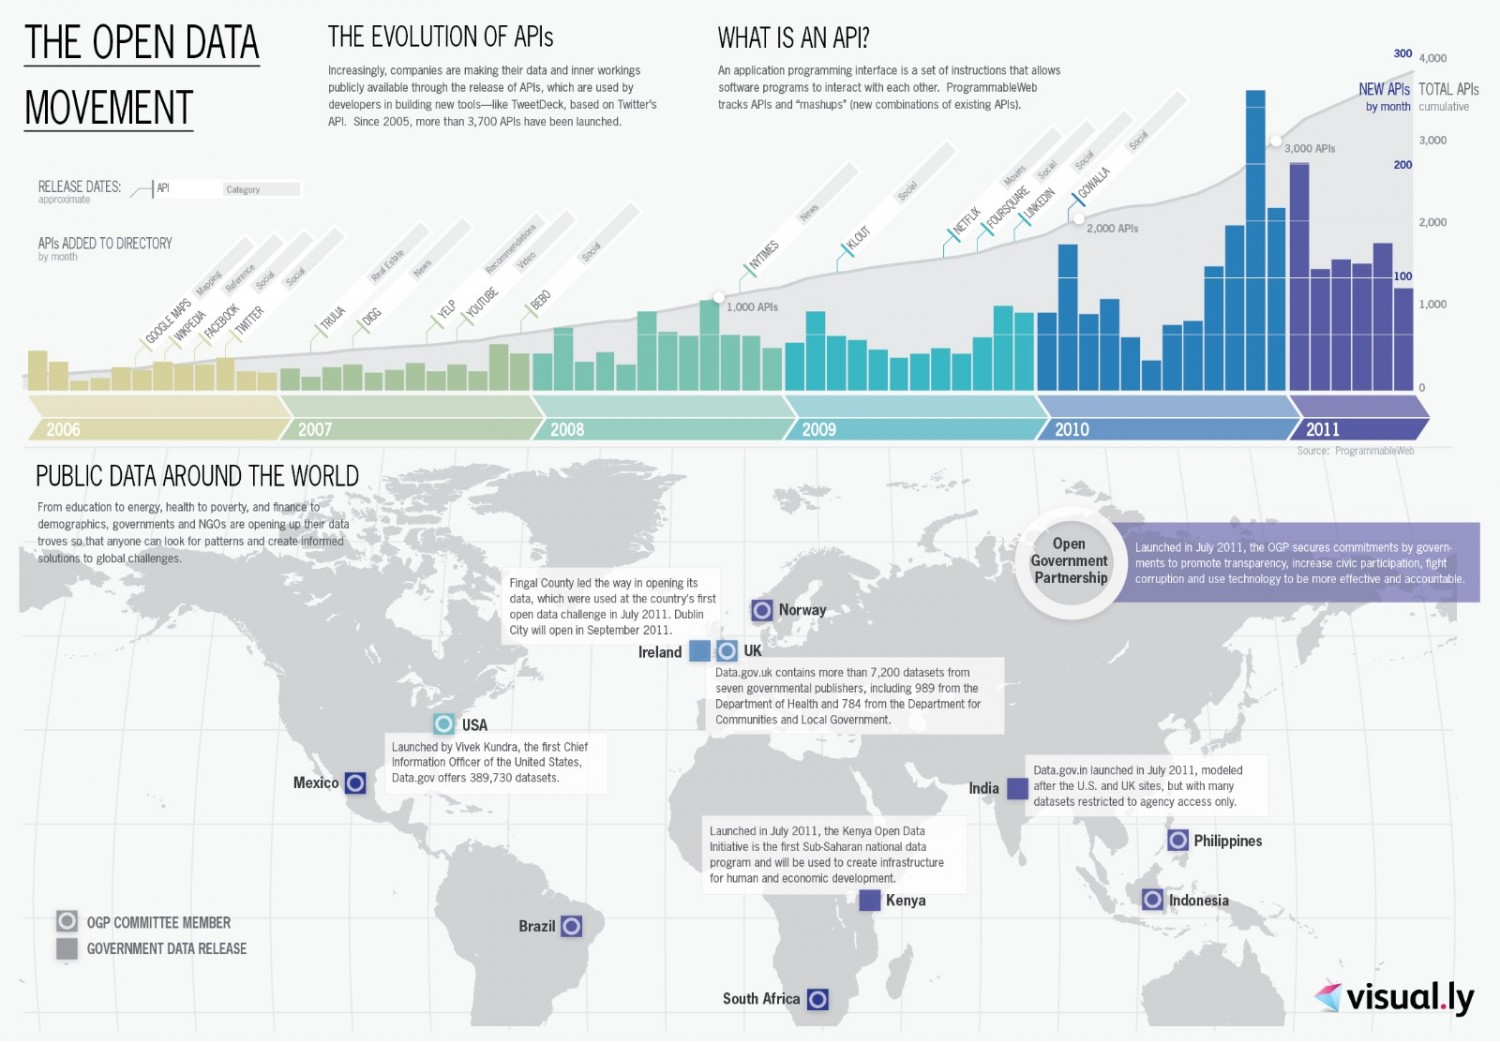
\includegraphics[scale=0.3]{graphics/opendata}
\end{figure}



Se estima que la apertura de datos, solo en Estados Unidos, puede generar entre 3 y 5 billones de dólares \cite{revenueOpenData}. El principal motivo es el gran potencial económico que puede suponer, ya que se podría aumentar la eficiencia en diferentes aspectos de la sociedad, como en la sanidad y educación, además, crearía nuevos servicios y productos, que irían acompañados de puestos de trabajo, y podrían mejorar la percepción para las personas sobre el mundo en general al aumentar la transparencia de la información.

Por otro lado en Europa, otros estudios prevén que el uso de datos abiertos reportará un ahorro de más de 1.7 billones de euros a las administraciones públicas, reducirá en un 16\% la energía consumida y el tiempo de espera en las carreteras. Aparte, indica que las compañías que siguen una filosofía de datos abiertos aumentan su valor en mayor medida que otras que no los abren \cite{valueOpenData}.

Por tanto, se espera que en el futuro cercano más y más países y organizaciones se sumen a estas iniciativas de apertura de datos y, que, los países que ya están participando en ellas, mejoren la calidad de la información que suministran, cuyos formatos, en ocasiones, no pueden ser utilizados sin una transformación a otros adecuados para la lectura por las máquinas.

\begin{figure}[htp!]
	\centering
	\caption{Valor potencial de los datos abiertos en billones de dólares en Estados Unidos}
	\label{fig:revenue}
	\vspace{5pt}
	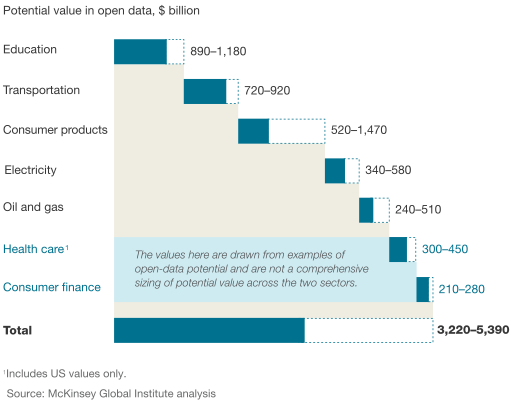
\includegraphics[scale=0.8]{graphics/revenue}
\end{figure}


\newpage
\section{Big Data}
\subsection{Introducción}
El término \textit{big data} es relativamente reciente, su primera aparición parece datar de 1989 cuando Erik Larson lo utilizó en una artículo para la revista Harper's, aunque, se creé que se definió como tal en los años noventa durante las charlas que daba John Mashey, científico jefe de Silicon Graphics, donde explicaba el término para vener sus productos, como se puede ver en presentaciones suyas de 1998 \cite{originbd}.

Sin embargo, los pilares en los que se basa el \textit{big data} no son nada nuevos. Los seres humanos nos hemos caracterizado por la idea de almacenar toda la información posible para crear una base de datos en continúa expansión que pueda ser analizada y de donde se extraiga conocimiento valioso para la humanidad.

Ya en el año 18000 \gls{AC}, había tribus paleolíticas que mediante muescas en palos y huesos hacían seguimientos de las reservas de suministros y de las actividades comerciales, permitiendo hacer predicciones sobre la duración de los alimentos almacenados. También, sobre el año 2400 \gls{AC} surge el ábaco en Babilonia que permitía realizar cálculos.

Como ejemplo de primer almacén de datos, tenemos a la Biblioteca Real de Alejandría, que fue la colección de conocimiento del antiguo mundo. Como primer ejemplo que definió el término ``Business intelligence'', contamos con el banquero Henry Furnese que utilizó en 1985 los datos recolectados de su negocio para obtener una ventaja competitiva frente a sus adversarios.

Pero es durante la segunda mitad del siglo XX y el XXI donde se produce los avances que han permitido llegar a la realidad actual. Hitos como el desarrollo de la computación, los sistemas de almacenamiento digital e Internet y las conexiones inalámbricas han sido las que han permitido crear y almacenar grandes cantidades de datos, unas cantidades que crecen exponencialmente con el tiempo.

\subsection{Definición \label{defBigData}}
Si buscamos la definición de \textit{big data} en Internet podemos encontrar diversas versiones de la misma \cite{ayuso}, algunas más correctas y otras menos, pero no existe un consenso claro sobre el término. Sin embargo, la agencia de la \gls{ONU} encargada de las tecnologías de la  información, creadora del primer estándar \textit{big data} lo define como un paradigma que permite la recolección, almacenamiento, manejo, análisis y visualización de extensos conjuntos de datos, con características heterogéneas y con restricciones de tiempo cercanas al tiempo real \cite{estandar}. 

Otro aspecto que ejemplifica estos cambios en la definición del concepto se puede apreciar en la conocida forma de describir el \textit{big data}, las V's. Estas comenzaron siendo tres \cite{ayuso}, para pasar a ser 4 \cite{4v} y, luego, 5 \cite{monse}, 7 \cite{soriano} e, incluso, 10. En la figura \ref{lasv} se puede apreciar como ha sido este proceso a lo largo del tiempo.

\begin{figure}[htp!]
	\centering
	\caption{Evolución de las V's que definen el \textit{big data} a lo largo del tiempo \cite{fotoV}}
	\label{lasv}
	\vspace{5pt}
	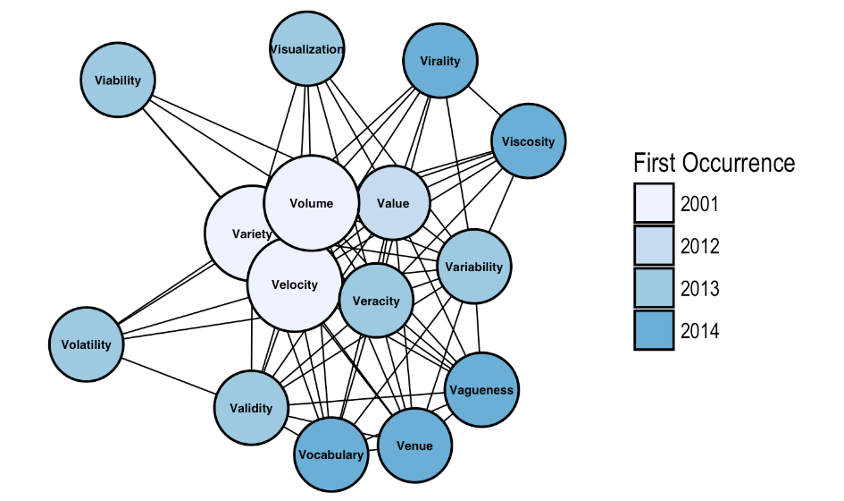
\includegraphics[scale=0.5]{graphics/lasv}
\end{figure}

Aunque, igual que en el caso de la definición, el número de V's variará dependiendo del experto al que consultes, podemos establecer cuatro aspectos básicos de un sistema para que este sea considerado \textit{big data}. Estos son:

\begin{itemize}
	\item \textbf{Volumen:} Referido como al tamaño y la cantidad de los datos, aunque no existe un límite establecido ya que estas cantidades cada vez aumentan a un mayor ritmo.
	
	\item \textbf{Velocidad:} Referido a la rapidez con la que se accede a los datos. Lo que se busca en un análisis en tiempo real.
	
	\item \textbf{Veracidad:} Referido a la certeza de que los datos contenidos en el sistema son reales. Un sistema \textit{big data} debe procurar mantener a cero la información no veraz a razón de no perder eficiencia.
	
	\item \textbf{Variedad:} Referido al número de fuentes diferentes de donde provienen los datos. Los sistemas \textit{big data} tienen que poder procesar datos de diversos orígenes y estructuras.
\end{itemize}

\clearpage
\subsection{Propósitos}
Muchas grandes compañías del sector tecnológico llevan años usando herramientas \textit{big data} para mejorar su negocio, compañías pioneras en este campo como Google y Yahoo que desarrollaron primeras versiones de esta tecnología buscando mejorar el resultado de sus buscadores.

Como ya se ha comentado anteriormente, las posibles aplicaciones de estas herramientas son infinitas. En general, disponer de un conjunto de datos que contengan información sobre situaciones pasadas o sobre sucesos y elementos que puedan influenciar un proceso es beneficioso para saber como actuar de la forma más correcta posible.

En general, se pueden encontrar cuatro tipos de usar herramientas \textit{big data} \cite{tipoAnalisis}. Por un lado, podemos encontrar el análisis prescriptivo, que es el más valioso y menos usado, que consiste la utilización de los datos para encontrar posibles caminos de actuación que permitan anticiparse al futuro y obtener ventaja. Un caso donde se está empezando a utilizar este tipo de análisis es en los sistemas de salud, donde conociendo los datos de un grupo, se pueden encontrar patrones para atajar enfermedades de la forma más efectiva.

Otro tipo de análisis es el predictivo, donde se busca detectar patrones que hayan ocurrido en el pasado para predecir el futuro. Este, está siendo especialmente utilizado en los procesos de venta, por ejemplo, para ajustar los precios en base a la oferta y la demanda, así como para preparar los ``stocks'' de los productos.

El análisis de diagnóstico es aquel que busca determinar porque se ha producido algún suceso, usando para ello los datos relacionados con el evento. Este es especialmente utilizado en marketing, para entender el efecto que han tenido las campañas, pero, también en sistemas de software, para conocer el motivo del error y poder evitar situaciones similares en el futuro.

Finalmente, el análisis descriptivo o minería de datos, que busca información valiosa entre todos los datos almacenados. Un ejemplo de este tipo de análisis se da en el estudio de los riesgos al ofrecer un crédito, donde se puede buscar en el pasado financiero del cliente datos que puedan describir la capacidad económica del mismo.

\clearpage
\subsection{Visión de negocio y futuro}
La amplias posibilidades que las herramientas \textit{big data} ofrecen junto con el conocido éxito de empresas y su, cada vez, más sencilla implementación está haciendo que cada vez más y más negocios implementen estas tecnologías.

El ``landscape'' también ha ido creciendo durante estos últimos años, debido al auge de estas tecnologías, haciendo que las herramientas y arquitecturas disponibles haya aumentado, disponiéndose de un amplio abanico de opciones que se adaptan a todo tipos de datos y análisis. En la figura \ref{landscape} se puede observar el panorama actual.

\begin{figure}[htp!]
	\centering
	\caption{Panorama de las tecnologías \textit{big data} en 2017 \cite{landscape}}
	\label{landscape}
	\vspace{5pt}
	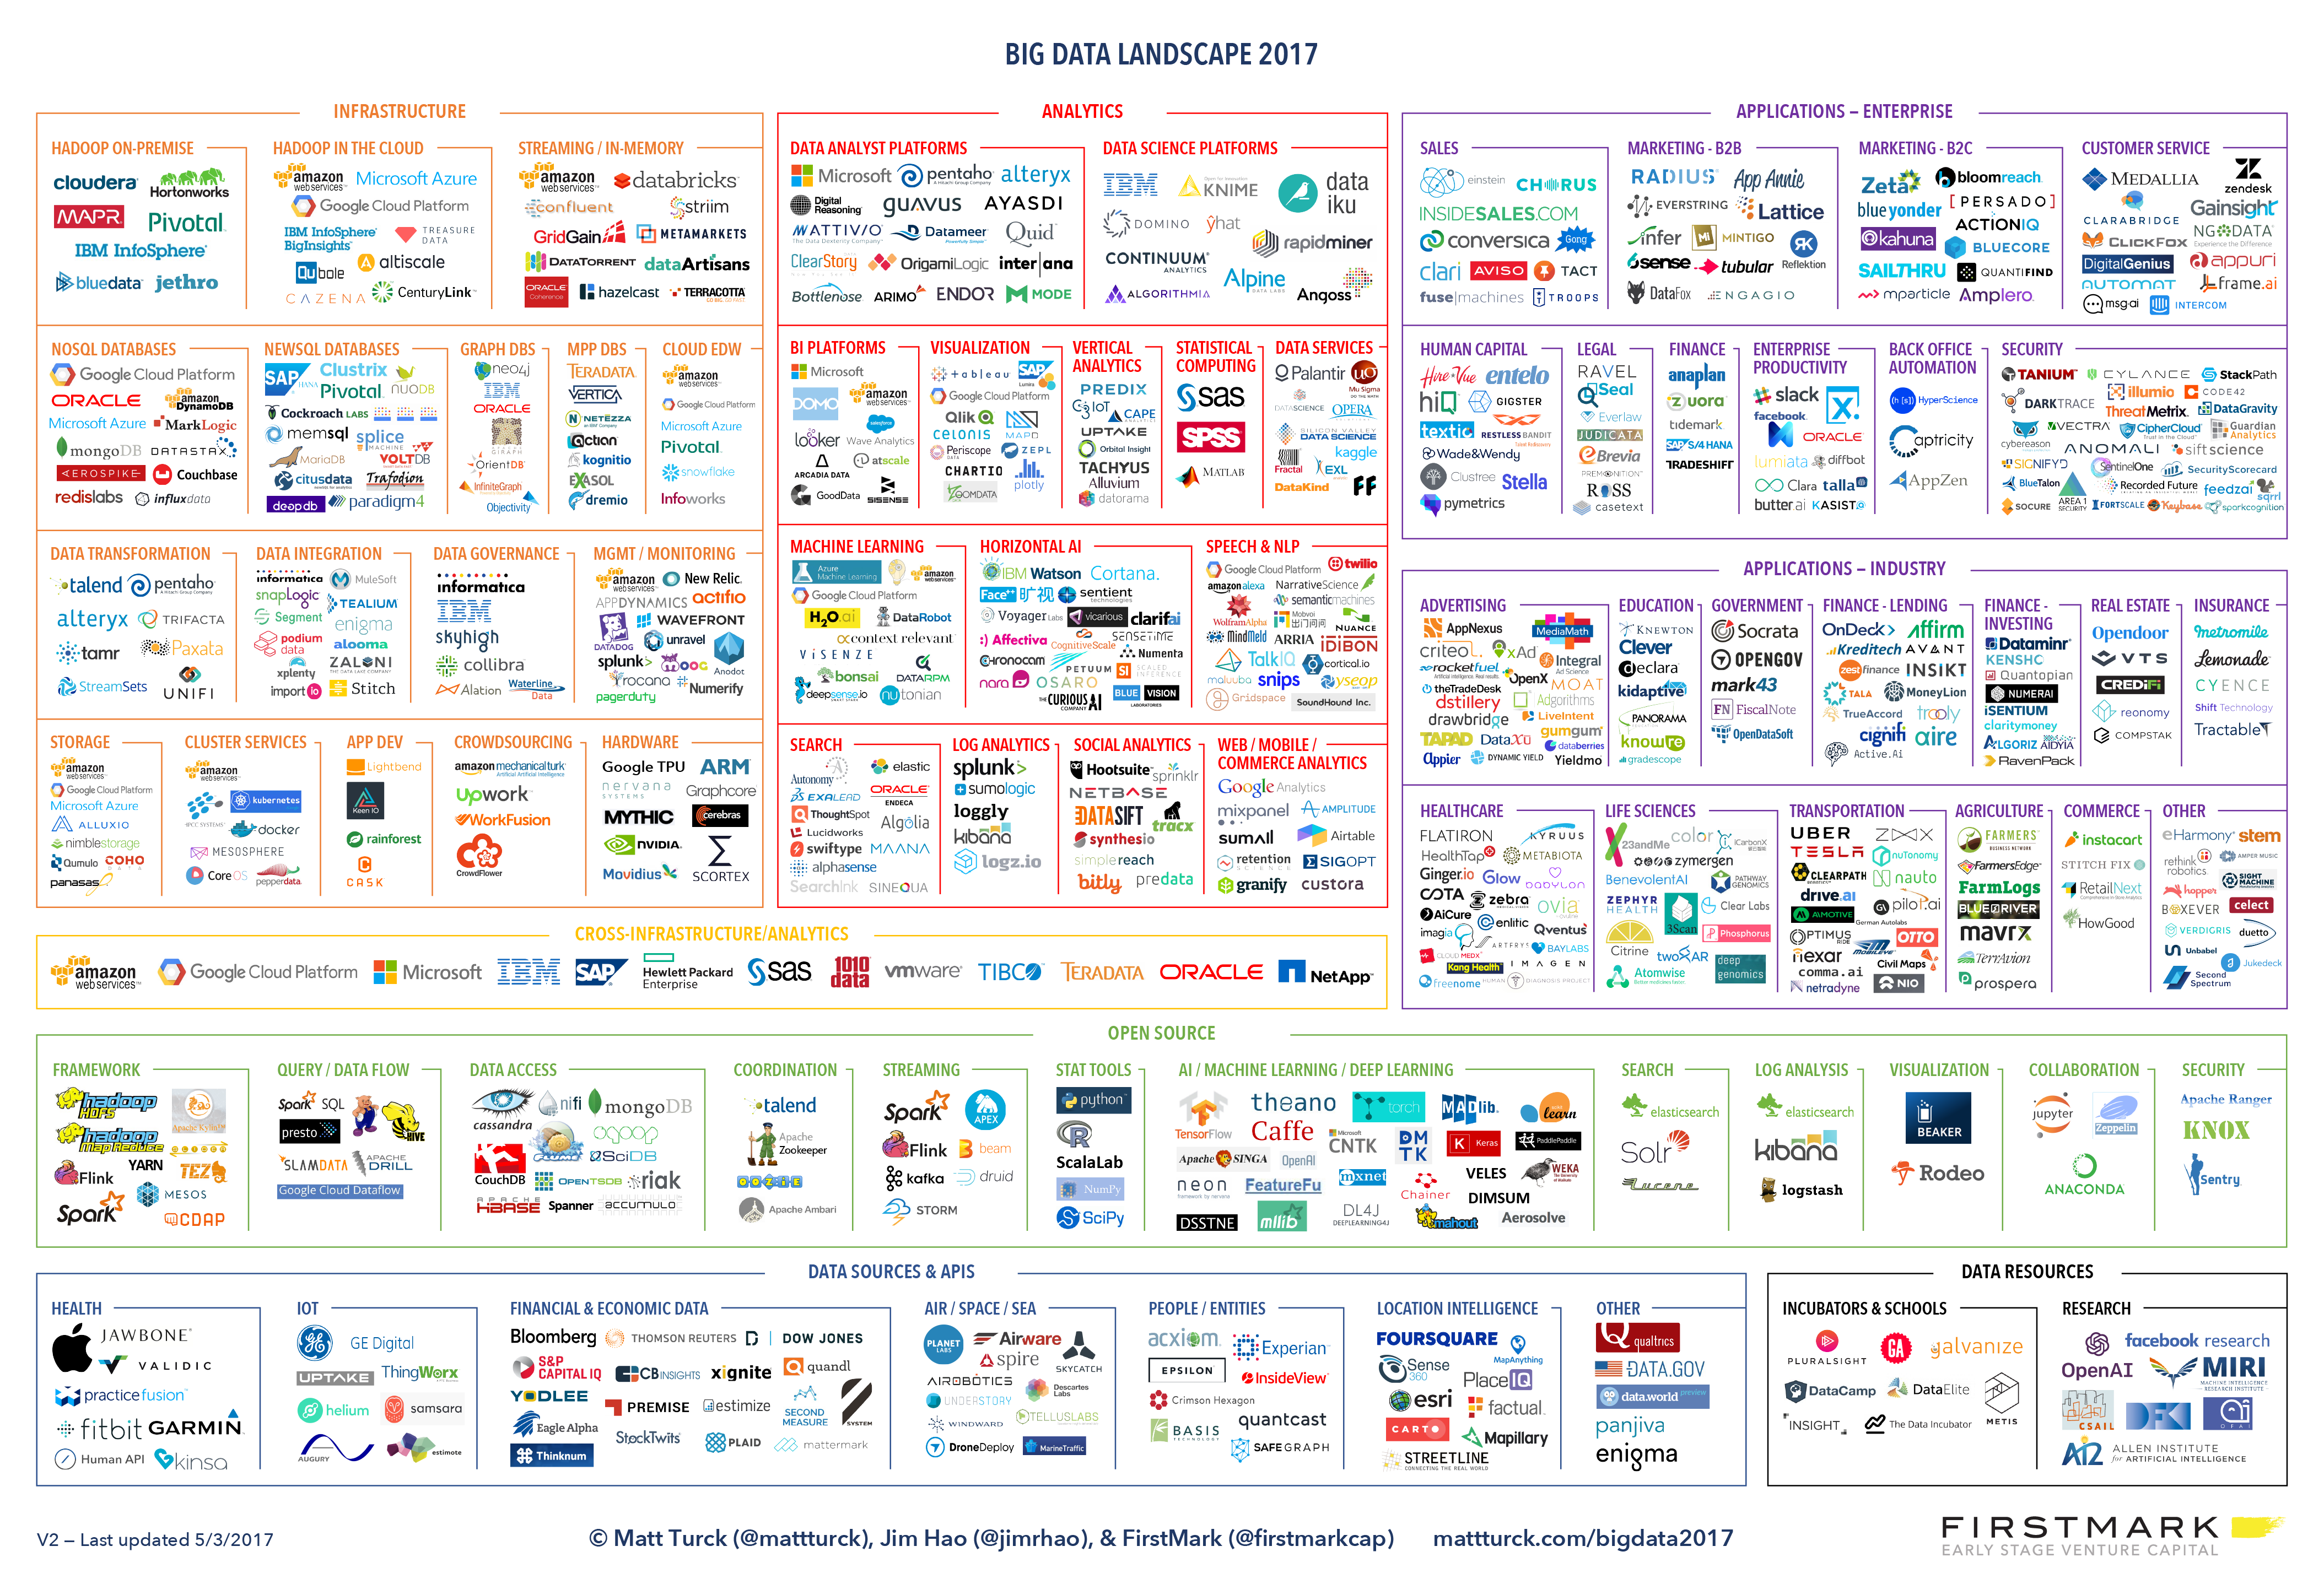
\includegraphics[scale=0.22]{graphics/landscape}
\end{figure}


Una de las características de este paradigma tecnológico es la naturaleza abierta de las herramientas, donde las más usadas son de código abierto y han surgido del resultado de la colaboración de diferentes empresas u organizaciones. Librerías como \textit{Apache Hadoop} \cite{hadoop} o \textit{Apache Spark} \cite{spark}, bases de datos como \textit{Apache Cassandra} \cite{cassandra} o \textit{MongoDB} \cite{mongo} y herramientas de análisis como \textit{SciPy} \cite{scipy} o \textit{Pandas} \cite{pandas} son de uso libre y no requieren de pago de licencias.

Esto ha hecho surgir empresas que se encargan de establecer y mantener un sistema \textit{big data}, es decir, ha permitido a los negocios externalizar este proceso, ahorrándose el presupuesto del diseño y la implantación de estos sistemas. Empresas como Hortonworks \cite{horton}, Cloudera \cite{cloudera} o Databricks \cite{databricks}, ofrecen sistemas de análisis de datos a empresas que utilizan las herramientas mentadas anteriormente, centrando su negocio en el cobro por el uso de recursos computacionales y el servicio técnico.

A este tipo de servicio que ofrecen estos negocios se les conoce como \gls{BDaaS} y se definen como servicios en la nube que permiten al usuario la capacidad de recoger, almacenar, analizar, visualizar y manejar los datos usando \textit{big data}.

El futuro del \textit{big data} parece prometedor, como se puede apreciar en la figura \ref{forecast}, proyectándose un crecimiento del 14.4\% anual en los ingresos generados por el \textit{big data}, pasando de los 18 billones de dólares en 2014 a los 92 en 2022. En general, las estadísticas de crecimiento son muy favorables para este sector tecnológico, con predicciones de entre el 4\% al 15\% \cite{forecast}.

Sin embargo, las tecnologías \textit{big data} no solo mejorarán los resultados económicos de las empresas. Estas, influirán directamente en los usuarios, mejorando las relaciones de estos con los servicios, principalmente, mediante la personalización de estos en base al cliente. También aumentarán la transparencia, al disponerse de más datos, permitiendo al usuario tener más conocimiento sobre las opciones disponibles.

\begin{figure}[htp!]
	\centering
	\caption{Proyección de los ingresos del \textit{big data}  \cite{forecast}}
	\label{forecast}
	\vspace{5pt}
	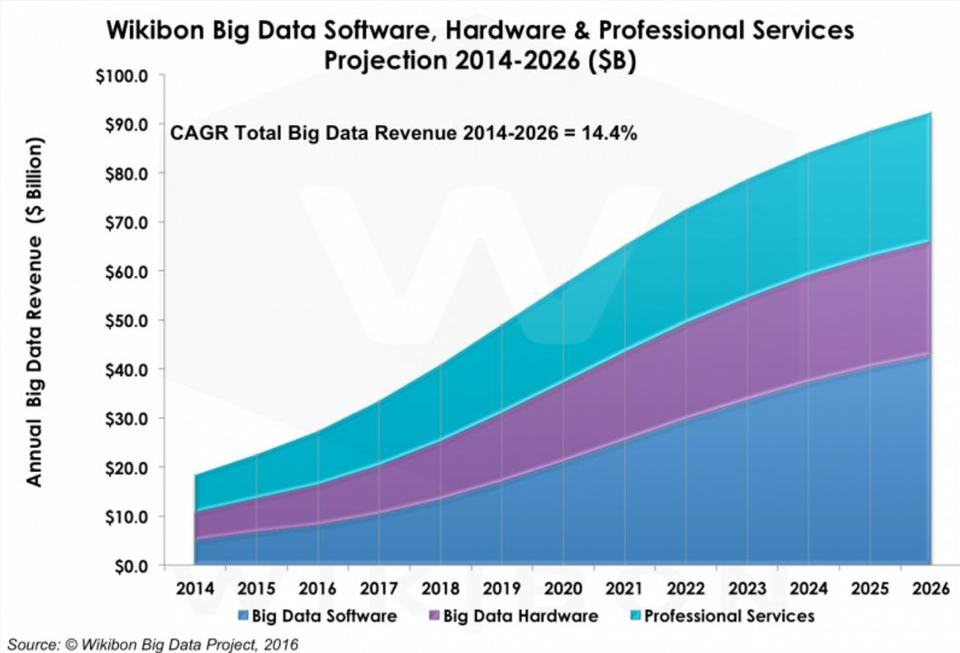
\includegraphics[scale=0.49]{graphics/forecast}
\end{figure}

\section{Sistemas distribuidos}
La computación distribuida es un modelo de computación que consiste en la conexión de diferentes máquinas, que pueden estar en localizaciones físicas distintas, con el fin de realizar tareas en un tiempo menor del que necesitaría una sola máquina. Es decir, un sistema distribuido es una red de equipos autónomos que se comunican entre ellos para conseguir un objetivo. Estos son independientes en el sentido que no comparten memoria o procesadores físicamente \cite{computacionDistribuidad}.

Estos ordenadores se comunican entre ellos por ``mensajes'' que son fragmentos de información que se intercambian por la red. Estos mensajes sirven para ordenar diferentes tareas con argumentos particulares, para enviar y recibir paquetes de datos o para mandar ordenar comportamientos específicos de otros ordenadores. Estas máquinas pueden tener diferentes roles dentro del sistema, dependiendo de su objetivo. 

\begin{figure}[htp!]
	\centering
	\caption{Esquema de computación distribuida \cite{fotodistribuida}}
	\label{distribuida}
	\vspace{5pt}
	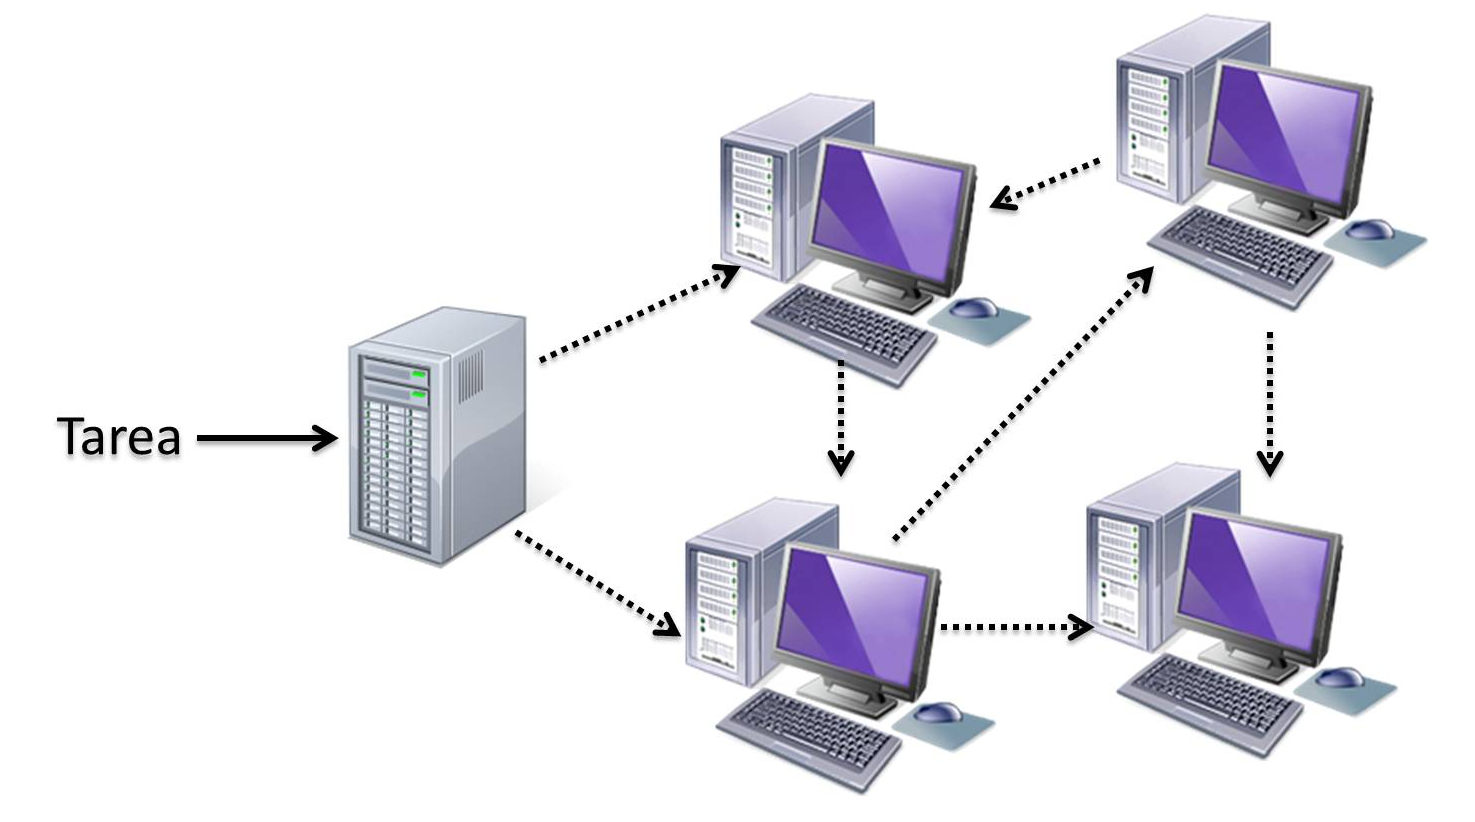
\includegraphics[scale=0.3]{graphics/computaciondistribuida}
\end{figure}

Las ventajas que ofrece este tipo de computación son \cite{sistDistTeoria}:

\begin{itemize}
	\item \textbf{Compartición de recursos:} Este modelo de computación permite que las máquinas compartan recursos de hardware al estar conectadas en red.
	
	\item \textbf{Escalabilidad:} Gracias a la capacidad de compartir recursos, nuevos sistemas pueden ser añadidos a la red y aumentar la capacidad del conjunto.
	
	\item \textbf{Tolerancia a fallos:} Al contarse con varias máquinas, la caída de alguna de ellas de la red no será crítico, permitiendo la continuidad del sistema.
	
	\item \textbf{Concurrencia:} Este modelo permite que se ejecuten varios procesos al mismo tiempo dentro de la red.
	
	\item \textbf{Variedad:} Se pueden incorporar máquinas con diferente hardware y software debido al uso de protocolos estándar.
\end{itemize}

A pesar de estas ventajas, también cuenta con inconvenientes como los siguientes:

\begin{itemize}
	\item \textbf{Complejidad:} Por el hecho de que se cuenta con varias máquinas, la organización y control de estos sistemas es más complicado que el de una sola máquina.
	
	\item \textbf{Seguridad:} Debido a que existen conexiones remotas que conectan a los equipos del sistema, se puede dar el caso de escuchas e interceptación de mensajes.
	
	\item \textbf{Disparidad en el comportamiento:} Se puede dar el caso de obtención de resultados diferentes dependiendo de las condiciones.
\end{itemize}

\subsection{Configuraciones}
Existen dos arquitecturas predominantes para la creación de sistemas distribuidos, la configuración cliente-servidor y la ``peer-to-peer''.

\subsubsection{Cliente-servidor}
La arquitectura cliente-servidor es una forma de ofrecer servicios desde una fuente central, es decir, existe un solo servidor a los que múltiples clientes se conectan para consumir sus productos. 

\begin{figure}[htp!]
	\centering
	\caption{Esquema cliente-servidor  \cite{computacionDistribuidad}}
	\label{clientserver}
	\vspace{5pt}
	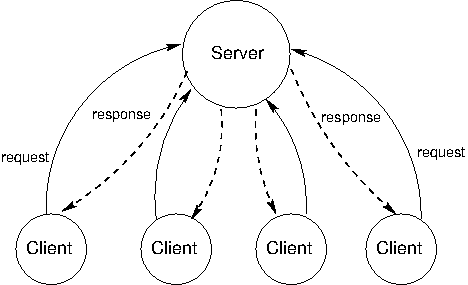
\includegraphics[scale=0.6]{graphics/clientserver}
\end{figure}

En este tipo los roles de los equipos son diferentes, mientras que el servidor es responder a las peticiones de los clientes, el trabajo de los clientes es usar los datos recibidos desde el servidor para realizar alguna tarea.

Internet es un ejemplo muy importante de este tipo de arquitectura ya que esta basada en ella, donde el servidor es una máquina que ofrece la página web a los sistemas que se conectan con ella. Sin embargo este sistema tiene dos importantes inconvenientes, por un lado, si se cae el servidor se paraliza el servicio totalmente. Por otro, este modelo no tiene capacidad de escalar, por lo que cuando hay muchos clientes conectados el rendimiento disminuye.

\subsubsection{Peer-to-peer}
Son aquellos sistemas distribuidos en los que el trabajo está dividido entre todos los componentes del sistema. Todos las máquinas envían y reciben datos y aportan capacidad de computación y memoria al sistema, siendo este más potente cuanto más integrantes tenga la arquitectura.

\begin{figure}[htp!]
	\centering
	\caption{Esquema peer-to-peer \cite{peertopeer}}
	\label{peertopeer}
	\vspace{5pt}
	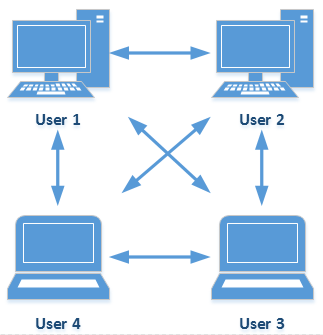
\includegraphics[scale=0.6]{graphics/peertopeer}
\end{figure}

La división del trabajo entre todos las máquinas es el aspecto clave de esta arquitectura y, para mantenerla, mantener un comunicación fiable es básico. Por ello, para asegurar que los mensajes llegan entre los componentes, la red de un sistema peer-to-peer es estructurada y todos los nodos del mismo tienen que procurar en tener suficiente información de la misma para mantenerlo.

Existen variaciones de este sistema donde hay elementos que se preocupan de mantener la conexión entre todos los equipos de la red, de controlar la información del sistema y proporcionarla y organizar las tareas del conjunto. Este tipo de sistema es el que utilizaremos en este proyecto, donde habrá un maestro que organizará las tareas y los esclavos que realizarán el procesamiento.

Las aplicaciones más comunes de este tipo de arquitecturas son la transferencia de datos y almacenamiento. También aplicaciones como Skype funcionan con esta tecnología.

\subsection{Arquitectura utilizada}
Como hemos comentado anteriormente, en este proyecto vamos a usar una variación de la arquitectura de sistemas distribuidos peer-to-peer, donde tendremos una máquina que hará de maestro y será la que se encargue de establecer la conexión con el resto de elementos, repartir las tareas y recolectar los datos. El resto hará de esclavos de esta máquina, realizando las tareas encargadas.

\subsubsection{Clúster o multinodo}
Un clúster es un conjunto de ordenadores conectados entre sí por una red de alta velocidad y que se comportan como si fueran un único sistema \cite{cluster}. 

\begin{figure}[htp!]
	\centering
	\caption{Esquema de un clúster \cite{clusterfoto}}
	\label{clusterDef}
	\vspace{5pt}
	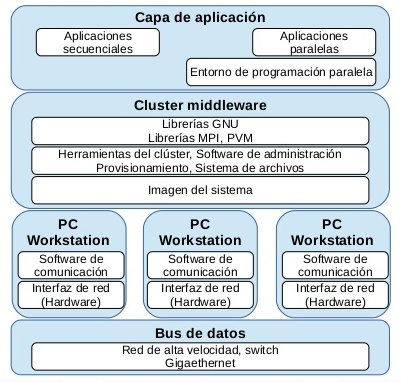
\includegraphics[scale=0.7]{graphics/clusterDef}
\end{figure}

La tecnología de clústeres es usada en tareas de cómputos o supercómputos, en servidores web y comercio electrónico y en bases de datos de alta disponibilidad. Es decir, las características de que se esperan de un clúster son las siguientes \cite{cluster}:

\begin{itemize}
	\item \textbf{Alto rendimiento:} Debido a que se trata de un conjunto de ordenadores, la suma de su potencia hace que sean óptimos para tareas que requieran gran capacidad de computación y sean paralelizables. 
	
	\item \textbf{Alta disponibilidad:} Por la misma razón, los clústeres deben ofrecer una rápida capacidad de recuperación ante fallos, por ejemplo, pudiendo recuperar los datos de un nodo perdido al guardar copias en otros o evitando la caída del sistema por el fallo en un nodo, siendo este sustituido.
	
	\item \textbf{Balanceo de carga:} Un clúster debe distribuir el trabajo entre todos los nodos de la manera más equilibrada posible.
	
	\item \textbf{Escalabilidad:} El sistema tendría que tener facilidad para adaptarse a las diferentes situaciones, siendo posible añadir o reducir capacidad del sistema mediante la adición o extracción de nodos del mismo.
\end{itemize}

Los elementos de un clúster son:

\begin{itemize}
	\item \textbf{Bus de datos:} Que conecta a los nodos del clúster y permite la comunicación entre ellos.
	
	\item \textbf{Nodos:} Es el conjunto de máquinas que forman el clúster, todas ellas tendrán que estar conectadas a la red y disponer de un software, el \gls{SO} que deberá ser multiproceso y multiusuario.
	
	\item \textbf{Middleware:} Que permitirá el entendimiento entre las aplicaciones y el sistema operativo de los nodos. Es el encargado de hacer que el clúster sea visto por el usuario como una única entidad y, por otro lado, es el encargado de realizar el balanceo de tareas y permitir la escalabilidad del sistema.
\end{itemize}

\subsection{Nuevos roles de trabajo}
Los datos se han convertido en un nuevo modelo de negocio por derecho propio, esto propicia la aparición de empresas dedicadas a ellos y por tanto nuevos roles de trabajo. Estos precisan de gente especializada en diferentes áreas para poder llevar a cabo estas fases de análisis y procesos.

\begin{itemize}
	\item \textbf{Data Scientist:} Este perfil es el encargado de la extracción de valor y conocimiento de los datos, donde debe analizar la información, realizar modelos predictivos y realizar los diferentes reportes que sean necesarios. Para ello se requieren conocimientos de estadística, matemáticas, programación, \gls{ML}, bases de datos y un largo etc.
	
	\item \textbf{Big Data Engineer:} Perfil técnico responsable del flujo de información ``end-to-end'' desde un punto de vista técnico, donde principalmente se debe de encargar de integrar las diferentes fuentes de datos y desarrollar procesos de transferencia. En definitiva desarrolla, construye, prueba y mantiene bases de datos y sistemas de procesamiento de datos a gran escala.
	
	\item \textbf{Big Data Architect:} Perfil técnico encargado del diseño, despliegue y gestión de la arquitectura \textit{big data}. Crea sistemas de gestión integrados para centralizar, proteger y mantener las fuentes de datos, se les requiere un profundo conocimiento del ecosistema \textit{Apache Hadoop} y \textit{UNIX} \cite{unix}.
	
	\item \textbf{Big Visualization Specialist:} Perfil responsable del diseño y creación de visualizaciones de datos de gran impacto, para ello se requiere conocimientos de arquitecturas webs, desarrollo de \gls{API}, conocimientos de ``full stack'' \cite{fullStack}, consultas a base de datos y herramientas comerciales de visualización.
	
	\item \textbf{Big Data Business Consultant:} Perfil responsable de la interlocución directa con el negocio, diseñar con el cliente la estrategia de implementación de la tecnología y el desarrollo de casos de uso analíticos para identificar las necesidades de negocio susceptibles de ser satisfechas con analítica avanzada de datos. Requiere conocimiento del sector y del negocio concreto, así como las tendencias de mercado y conocimientos sobre la tecnología \textit{big data}.	
	
\end{itemize}


\clearpage

\section{Infraestructura}
\subsection{Apache Spark \label{sparkEA}}
\textit{Apache Spark} \cite{spark} es un \gls{framework} de código abierto que permite el procesamiento de datos mediante la computación distribuida. Desarrollado originalmente por el departamento AMPLab \cite{amplab} de la Universidad de California, fue, posteriormente, donado a la fundación Apache, que lo ha mantenido desde entonces. 

Desarrollado en Scala \cite{scala} y con soporte para Java, Python y R, \textit{Apache Spark} proporciona una \gls{API} para programar clúster con paralelismo de datos implícito y tolerancia a fallos. Esta \gls{API} se apoya en la estructura llamada \gls{RDD}, donde se almacenan los datos particionados para permitir transformaciones en paralelo y que mantiene el índice de estas transformaciones para rehacerlas en caso de error.

Una buena característica de este \gls{framework} es el amplio soporte para la mayoría de los formatos de ficheros de datos, teniendo, además, integraciones con varios sistemas de almacenamiento como \gls{HDFS}, \textit{Apache Cassandra} \cite{cassandra} o Amazon S3 \cite{aws}. En la figura \ref{partSpark} podemos observar los diferentes componentes que conforman \textit{Apache Spark}.

\begin{figure}[htp!]
	\centering
	\caption{Componentes de \textit{Apache Spark} \cite{partsSpark}}
	\label{partSpark}
	\vspace{5pt}
	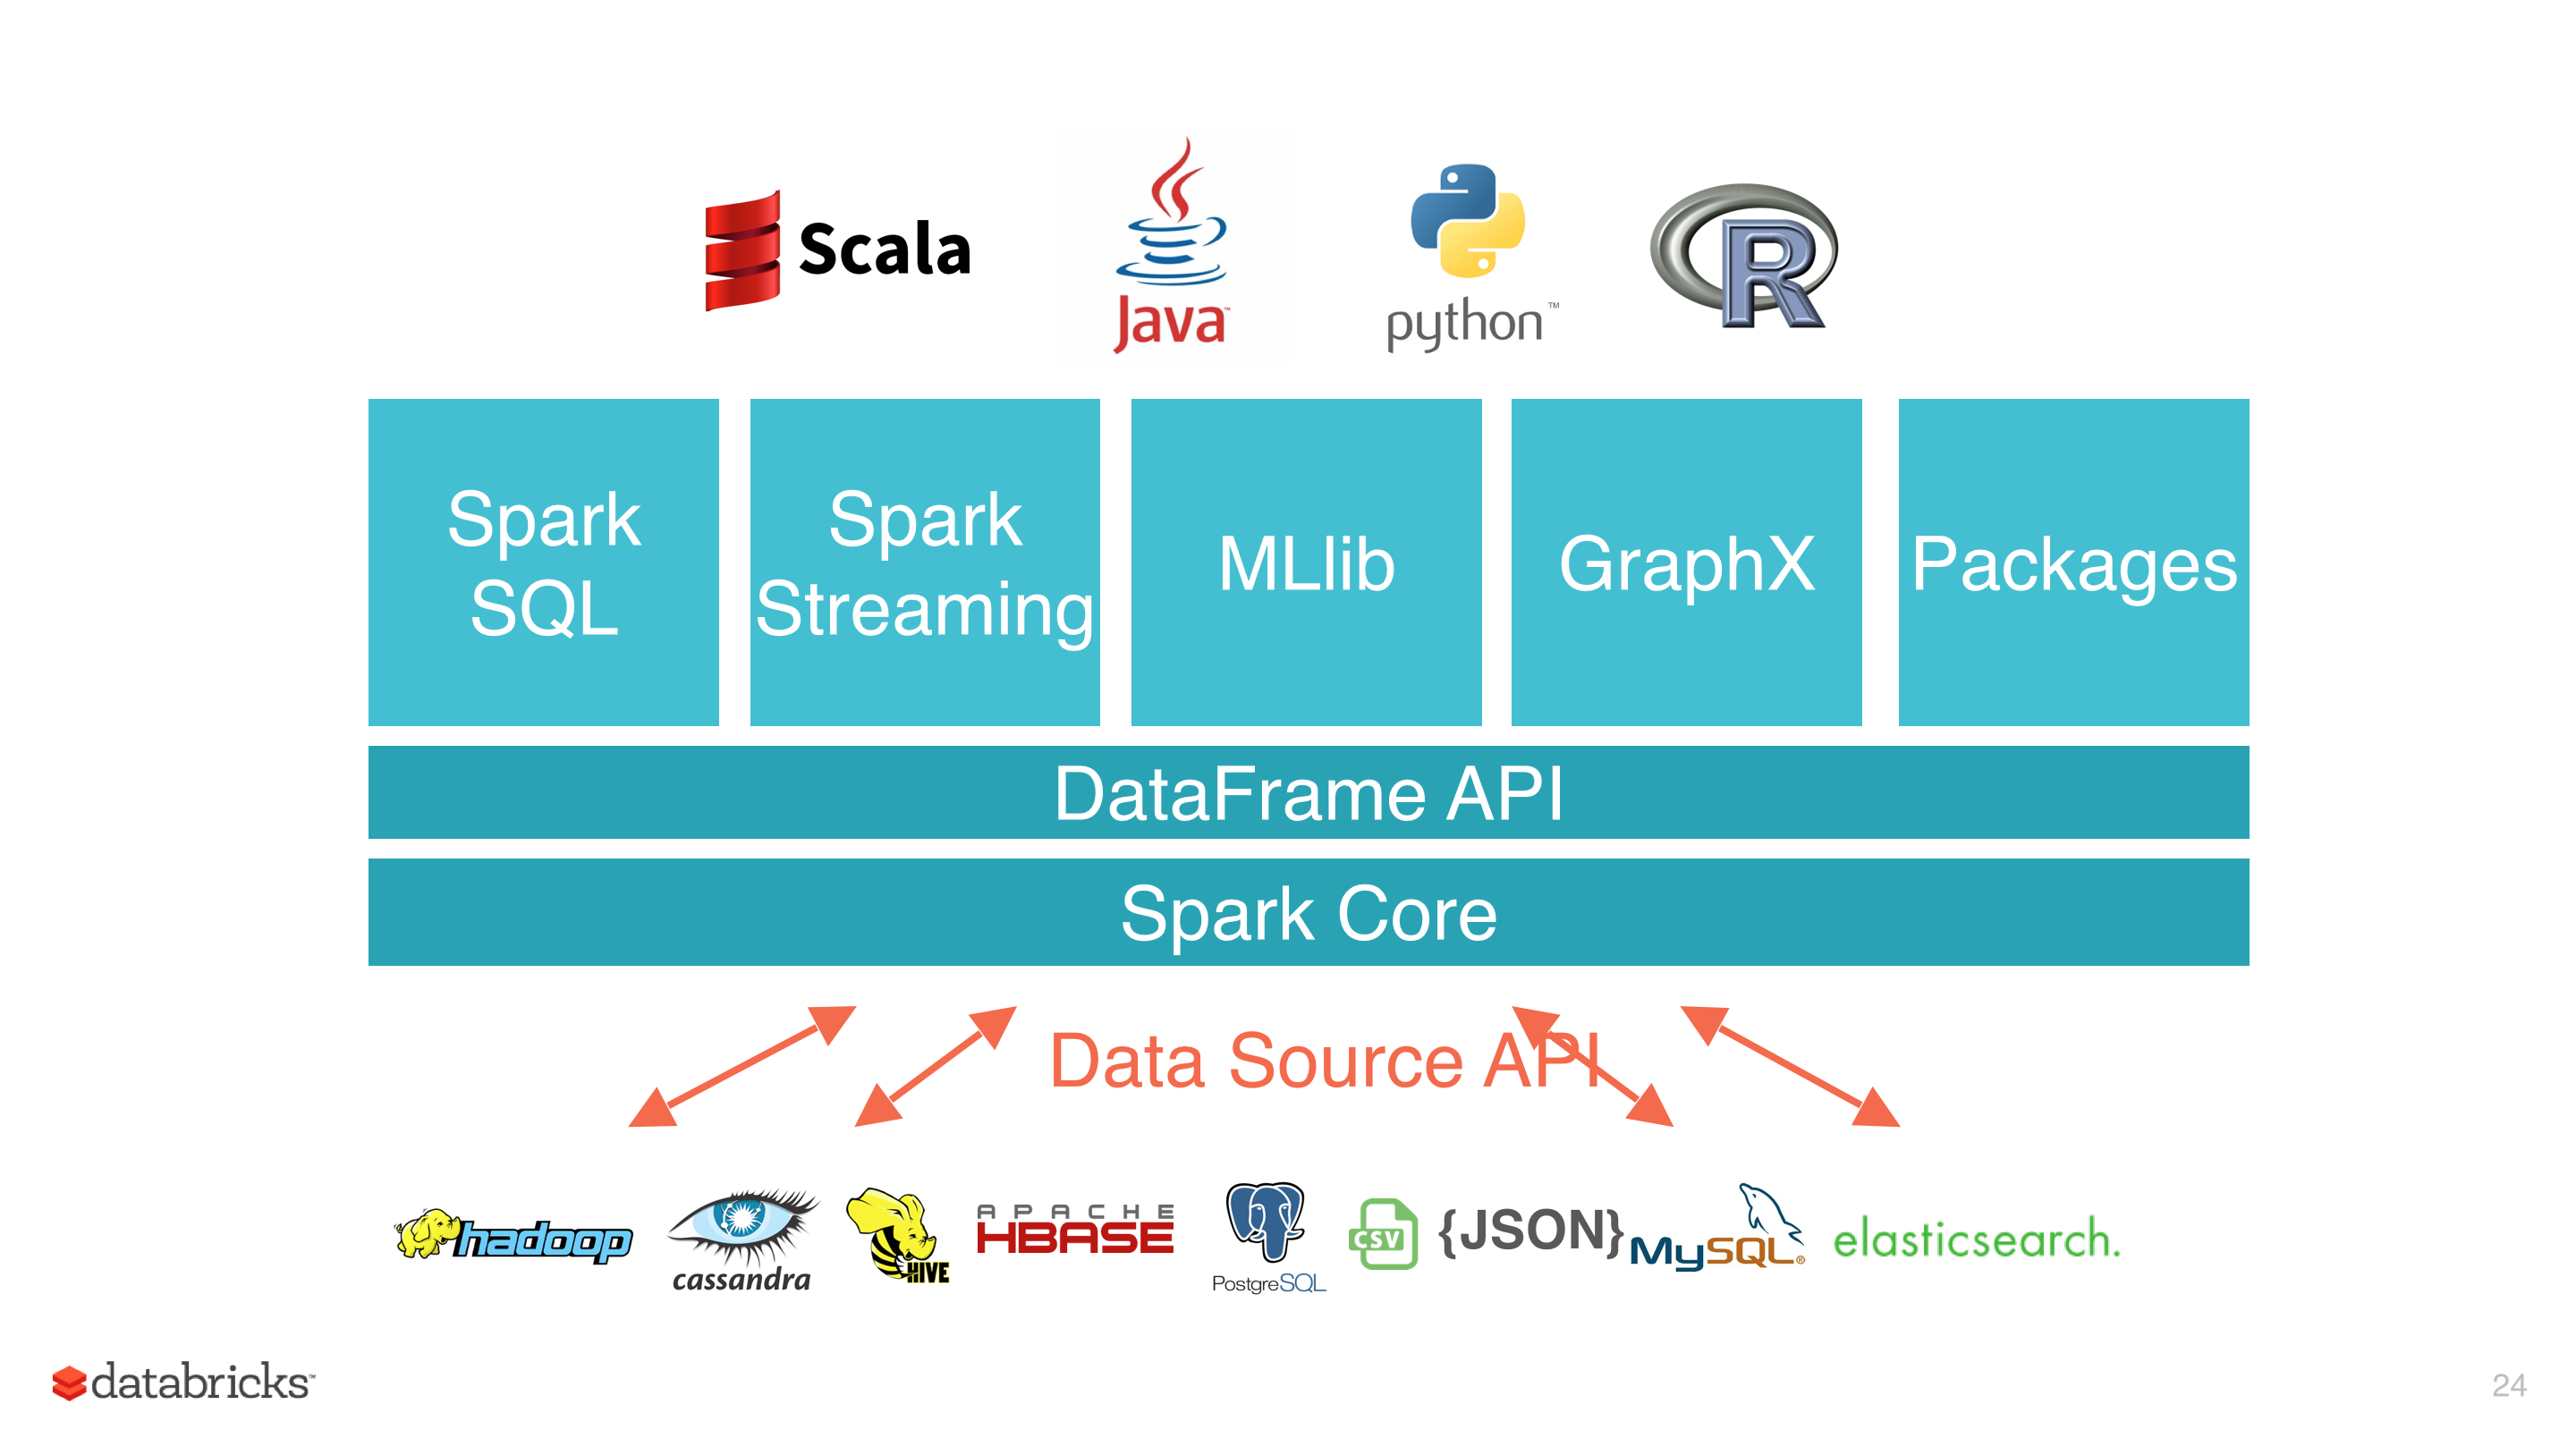
\includegraphics[scale=0.3]{graphics/partSpark}
\end{figure}

El \gls{framework} está formado por una base, sobre la que trabajan las diferentes librerías y paquetes del mismo. Dicha base está formada por el núcleo del programa, donde se crean y manipulan los \gls{RDD}, y la \textit{DataFrame} \gls{API}, que es una abstracción a más alto nivel de los \gls{RDD}, para simplificar su manipulación por el usuario.

Además \textit{Apache Spark} cuenta con diversas librerías como Spark SQL, para realizar consultas sobre los datos, Spark Streaming, para permitir la introducción y análisis de datos en tiempo real, MLib, para realizar aprendizaje automático, y Graphx, que permite la computación de grafos.

\subsubsection{Funcionamiento}
\textit{Apache Spark} basa su funcionamiento en dos conceptos, \gls{RDD} y \gls{DAG}. Una aplicación consiste en un controlador, llamado \textit{SparkContext}, que utiliza el código de usuario para crear y transformar \gls{RDD} y alcanzar el objetivo final. Estas transformaciones de los \gls{RDD}s son traducidos a gráficos \gls{DAG} para ser enviados al planificador y que este reparta las tareas.

\begin{figure}[htp!]
	\centering
	\caption{Funcionamiento de \textit{Apache Spark} \cite{partsSpark}}
	\label{sparkWork}
	\vspace{5pt}
	\includegraphics[scale=0.35]{graphics/sparkWork}
\end{figure}

\paragraph{\gls{RDD}: Resilient Distributed Dataset.}
Esta es la solución clásica en \textit{Apache Spark} para tratar los datos de una forma paralela y a prueba de errores. Además ofrece diferentes \gls{API}s para realizar transformaciones sobre los datos y permite el control sobre el modo de particionar los datos y el caché de los mismos.

Un \gls{RDD} puede ser creado a partir de un fichero en un almacenamiento externo o a partir de otro \gls{RDD} y es un sistema vago (\textit{lazy}), es decir, se guardan las operaciones que se realizarán sobre los datos, pero estas no son ejecutadas hasta que no se realiza la evaluación de los datos. Este sistema también es utilizado para la evitar los errores, donde el sistema sigue los pasos realizados desde el inicio para recomponer los datos correctamente.


Existen diferentes grupos de operaciones que se pueden realizar sobre un \gls{RDD}, estos son:

\begin{itemize}
	\item \textbf{Transformaciones:} Permite realizar las funciones codificadas por el usuario sobre todos los datos del sistema, permite operaciones de agrupación, ordenamiento y particionamiento del \gls{RDD}. Estas operaciones son reflejadas en el grafo \gls{DAG}.
	
	\item \textbf{Acciones:} Son las que inician el trabajo, es decir, hacen que se ejecuten las transformaciones estables
	
	\item \textbf{Persistencia:} Permiten almacenar el \gls{RDD} en memoria o en disco de forma explicita.
\end{itemize}

\paragraph{DataFrame.}
Esta es una variante de los \gls{RDD} incluida en el modulo \gls{SQL} que permite consultar los datos con una ``query'' como si se tratase de una base de datos.

En \textit{Apache Spark}, un \textit{DataFrame} es una colección distribuida de datos organizados en columnas nombradas. Es conceptualmente equivalente a una tabla en una base de datos relacional o un marco de datos en R/Python, pero con optimizaciones más ricas bajo el capó. Un \textit{DataFrame} se puede construir a partir de una amplia gama de fuentes como: archivos de datos estructurados, tablas en Hive, bases de datos externas o \gls{RDD} existente.

\paragraph{\gls{DAG}: Direct Acyclic Graph. \cite{dataframe}} 
Es la forma de codificación de los trabajos sobre los \gls{RDD}s o \textit{DataFrame} utilizada en \textit{Apache Spark}. Indica el flujo que seguirá la aplicación durante la ejecución que, generalmente, se basa en leer los datos del origen, realizar las transformaciones oportunas y materializar los datos obtenidos.

\begin{figure}[htp!]
	\centering
	\caption{Transformaciones sobre un \gls{RDD} representadas en un \gls{DAG} \cite{partsSpark}}
	\label{dag}
	\vspace{5pt}
	\includegraphics[scale=0.4]{graphics/dag}
\end{figure}

Este componente también es el que se encarga de establecer las diferentes tareas del trabajo que, posteriormente, serán repartidas entre los nodos del clúster para paralelizar el trabajo.

Una de las características que diferencia \textit{Apache Spark} es la forma en la que gestiona los datos, este \gls{framework} guarda los datos en la memoria \gls{RAM} del dispositivo, sin llegar escribir a disco, por lo que el acceso a estos es muy rápido. Por ello, hace que la velocidad en procesos iterativos, donde se consultan los mismos datos de forma continua, sea muy elevada, mejorando con creces los tiempos de otros sistemas como MapReduce \cite{compSpark}.

\begin{figure}[htp!]
	\centering
	\caption{\gls{RDD} distribuido en diferentes máquinas \cite{sparkdistributed}}
	\label{rdddistribuido}
	\vspace{5pt}
	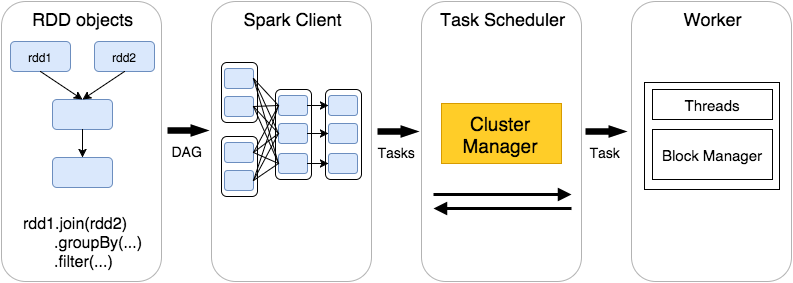
\includegraphics[scale=0.55]{graphics/rdddistribuido}
\end{figure}

\clearpage
\subsubsection{Librerías}
Como se ha indicado anteriormente, \textit{Apache Spark} incluye diferentes librerías o módulos que trabajan sobre la base del \gls{framework}. Estas son:

\begin{itemize}
	\item \textbf{Spark SQL:} Permite el soporte para datos estructurados o semi-estructurados para realizar consultas \gls{SQL} sobre ellos. Estos datos pueden ser modificados con funciones específicas de \textit{Apache Spark} o mediante el lenguaje \gls{SQL}.
	
	\item \textbf{Spark Streaming:} Permite el análisis en tiempo real de datos mediante la introducción de estos en mini lotes de datos. Este sistema aunque cumple su función no es tan potente como el ofrecido por otras alternativas como \textit{Apache Flink} \cite{flink} o \textit{Apache Storm} \cite{storm}.
	
	\item \textbf{MLib:} Es un \gls{framework} de aprendizaje automático distribuido. Este permite diferente tipos de análisis sobre los datos: clasificaciones, regresiones, clusterizaciones, optimizaciones, etc.
	
	\item \textbf{GraphX:} Es un procesador de grafos distribuido. Es muy veloz para grafos que no tienen que ser actualizados, sin embargo, debido a la naturaleza inmutable de los \gls{RDD} no es una herramienta válida para grafos que se modifiquen.
\end{itemize}

\clearpage
\subsection{Apache Hadoop \label{hadoopEA}}
\textit{Apache Hadoop} \cite{hadoop} es otro \gls{framework} de código abierto que permite el tratamiento de grandes cantidades de datos de forma distribuida. Desarrollado en Java, permite la gestión de clústeres de un nodo hasta cientos de ellos de forma sencilla. Al establecer sistemas distribuidos estos tienen una alta tolerancia a los fallos.

\textit{Apache Hadoop} cuenta con cuatro módulos principales, aunque cuenta con muchos más proyectos totalmente compatibles: 

\begin{itemize}
	\item \textbf{Hadoop Common:} Utilidades comunes que soportan el resto de módulos.
	
	\item \textbf{Hadoop Distributed File System (\gls{HDFS})} Sistema de ficheros distribuido que permite la replicación de los datos en los nodos del sistema.
	
	\item \textbf{Hadoop YARN:} Es un \gls{framework} que se encarga de la gestión de los trabajos y los recursos del clúster.
	
	\item \textbf{Hadoop Mapreduce:} Sistema basado en YARN para el procesamiento paralelo de grandes cantidades de datos.
\end{itemize}

En este proyecto, debido a que utilizamos \textit{Apache Spark} para la gestión del clúster, no utilizaremos la mayoría de los módulos de \textit{Apache Hadoop}. El módulo que se utilizará será el sistema de ficheros \gls{HDFS} por la configuración distribuida del clúster doméstico. 

Con este sistema realizaremos la replicación de los ficheros de datos en los diferentes nodos del sistema y, de esa forma, ahorrar la transmisión de estos durante la ejecución de los trabajos y, así, mejorar los tiempos de procesamiento.

\subsubsection{Hadoop Distributed File System (\gls{HDFS})}
\gls{HDFS} es un sistema de ficheros distribuido, escalable y portable escrito en Java. Este permite el almacenado de grandes cantidades de datos mediante la distribución de estos en diferentes máquinas. \gls{HDFS} es muy tolerante a los fallos y esta diseñado para correr en hardware de bajo coste. 

\gls{HDFS} fue construido con las siguientes asunciones y objetivos:

\begin{itemize}
	\item \textbf{Errores de hardware:} Los fallos de hardware son más una norma que una excepción en la realidad, por ello, \gls{HDFS} es muy tolerante a los fallos, distribuyendo y replicando los datos en diferentes máquinas del clúster para no perder el acceso a ellos por la caída de algún nodo.
	
	\item \textbf{Acceso al streaming de datos:} \gls{HDFS} fue concebido para aplicaciones que necesitan un buen rendimiento en el acceso a los datos, más que para su manipulación continua por los usuarios. Por ello, se centra más en el procesamiento en lotes.
	
	\item \textbf{Grandes volúmenes de datos:} \gls{HDFS} está afinado para manejar ficheros de datos que van desde los cientos de gigasbytes hasta terabytes de tamaño.
	
	\item \textbf{Modelo de coherencia simple:} Las aplicaciones que usan este sistema necesitan el acceso a la lectura del fichero más que sus modificaciones. Por ello, el sistema del \gls{HDFS} usa un modelo ``escribe una vez y lee el resto'', por lo que una vez que se crea un fichero, se escribe y guarda, este no vuelve a modificarse excepto para reducir la cantidad de datos o añadir más.
	
	\item \textbf{``Mover la capacidad de computación es más barato que mover los datos'':} Una aplicación es más eficiente si la computación se realiza cerca de los datos, ya que ahorras el tiempo de transporte de estos. Esta es la premisa que sigue \gls{HDFS} y por ello se replican los datos en todos los sistemas para realizar las operaciones sobre estos en los propios nodos.
	
	\item \textbf{``Portabilidad entre hardware y software heterogéneo'': } \gls{HDFS} ha sido diseñado para ser fácilmente portado entre sistemas y plataformas.
\end{itemize}

\begin{figure}[htp!]
	\centering
	\caption{Arquitectura del \gls{HDFS} \cite{hadoop}}
	\label{hdfsarchitecture}
	\vspace{5pt}
	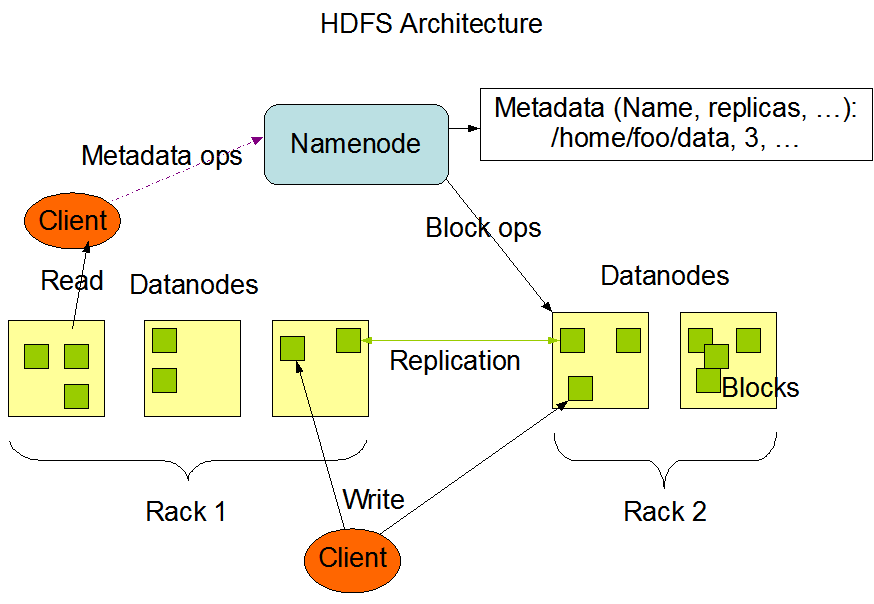
\includegraphics[scale=0.6]{graphics/hdfsarchitecture}
\end{figure}

En la figura \ref{hdfsarchitecture} podemos ver la arquitectura de un sistema \gls{HDFS}, este esta basado en la estructura maestro/esclavo, donde existe una \textit{Namenode} que hace de maestro y gestiona el sistema de ficheros y regula el acceso a los ficheros por los clientes. Por otro lado, están los \textit{Datanodes}, uno por nodo, que es donde se almacenan y gestionan los datos del sistema.

Por otro lado, dentro de estos \textit{Datanodes} encontramos los bloques, que son partes o fragmentos de los datos originales y que se replican por los diferentes nodos.

\subsection{Apache Flume \label{flume}}
\textit{Apache Flume} \cite{flume} es un sistema distribuido, seguro y eficiente para recoger, agregar y mover grandes volúmenes de datos provenientes de \textit{logs} desde distintas fuentes a un almacén de datos centralizado. \textit{Apache Flume} trabaja con agentes, que son procesos independientes que alojan los componentes de \textit{Apache Flume}.

\begin{figure}[htp!]
	\centering
	\caption{Arquitectura del \gls{HDFS} \cite{flumeArch}}
	\label{flumearchitecture}
	\vspace{5pt}
	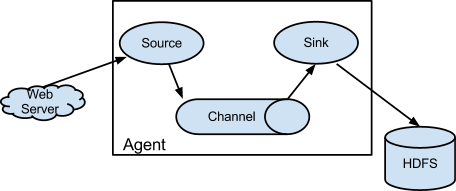
\includegraphics[scale=0.8]{graphics/flumearch}
\end{figure}

En la figura \ref{flumearchitecture} se pueden ver los componentes un agente de \textit{Apache Flume}. Estos están conformados de la siguiente forma:

\begin{itemize}
	\item \textbf{Evento:} Un \textit{payload} \cite{payload} de bytes con encabezados opcionales que representan la unidad de datos que Flume puede transportar desde su punto de origen hasta su destino final.
	
	\item \textbf{Cliente:} Implementación que opera en el punto de origen de los eventos y los entrega a un agente Flume. Por ejemplo, Log4J appender, es un cliente de Flume.
	
	\item \textbf{Fuente (\textit{source}):} Implementación que puede consumir eventos entregados a él a través de un mecanismo (por ejemplo, la monitorización de un directorio). Cuando una fuente recibe un evento, este se lo entrega a uno o más canales.
	
	\item \textbf{Canal (\textit{channel}):} Es un almacenamiento temporal para eventos, donde estos se entregan a través de la fuentes que operan con el agente. Un evento permanece en el canal hasta que es recogido por un sumidero (\textit{sink}).
	
	\item \textbf{Sumidero (\textit{sink}):} Implementación que puede eliminar eventos de un canal y transmitirlos al siguiente agente en el flujo, o hasta el destino final del evento.
\end{itemize} 

\clearpage
\subsection{Jupyter Notebook \label{jupyterEA}}
Jupyter \cite{jupyter} es un nuevo entorno de trabajo \textit{open source} oriente a científicos de datos que soporta los lenguajes R y Python, entre otros.

Jupyter surge en 2014 como una evolución del proyecto IPython \cite{iptyhon}, una potente consola vitaminada para Python. Sin embargo, Jupyter es mucho más ambicioso que IPython, se pretende construir una plataforma agnóstica del lenguaje que ofrezca a los científicos un conjunto de potentes herramientas para trabajar con datos, visualizarlos y poder compartir los resultados.

\begin{figure}[htp!]
	\centering
	\caption{Previsualización del entorno de Jupyter Notebook \cite{jupyter}.}
	\label{jupyterPreview}
	\vspace{5pt}
	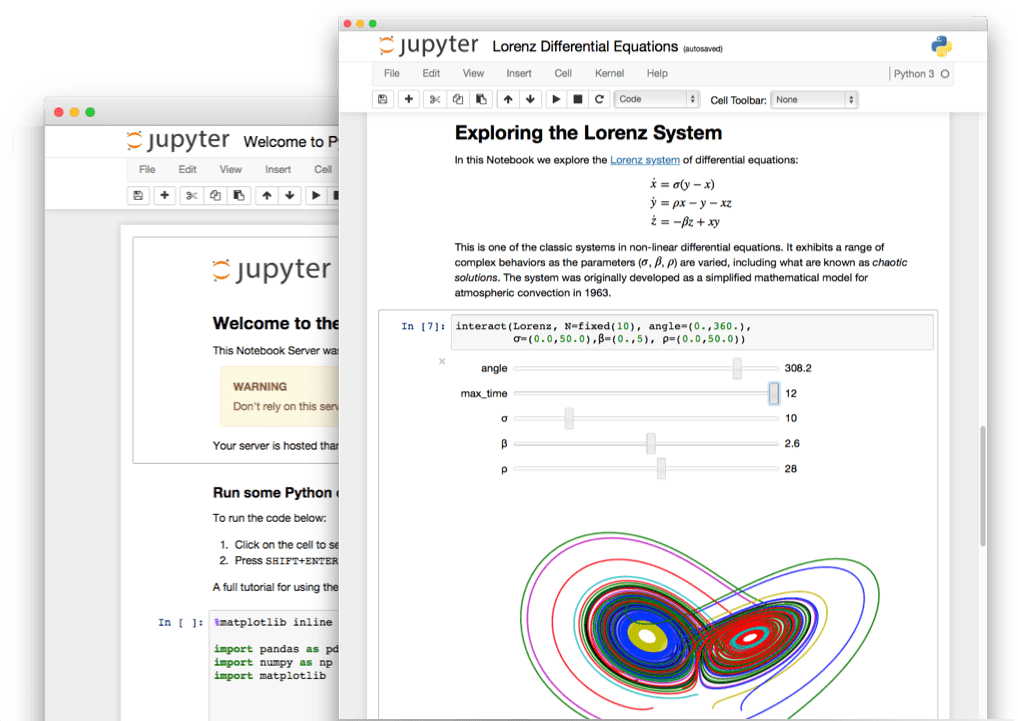
\includegraphics[scale=0.45]{graphics/jupyterpreview}
\end{figure}

Jupyter nos ofrece una shell interactiva vía web, a la que podemos acceder desde un navegador. La shell está organizada en pequeños bloques, cada bloque puede contener texto arbitrario formateado en Markdown \cite{markdown}, fórmulas matemáticas en LaTeX \cite{latex}, código en multitud de lenguajes, resultados, gráficos, vídeos, widgets o cualquier elemento multimedia.

Podemos escribir código de programación en estas celdas e ir ejecutándolo paso a paso o todo de golpe, obteniendo todos los resultados parciales. También podemos usar los bloques de texto para documentar el código o añadir las explicaciones oportunas, que pueden contener enlaces, imágenes, vídeos u otros elementos.

Esta serie de piezas de código, notas y resultados se guardan en un notebook, que es un fichero que contiene toda esta información. Uno de los principales objetivos de Jupyter es fomentar y simplificar la compartición de conocimiento y resultados a través de los notebooks. Plataformas como GitHub \cite{github} o Databricks Community \cite{databricks} facilitan esta tarea. De esta manera los notebooks pueden ser fácilmente difundidos y los resultados pueden ser reproducidos y validados en diferentes entornos. Por supuesto esto es muy útil para la divulgación y la formación o en entornos educativos.

Jupyter soporta integración con más de 40 lenguajes de programación en los que podemos escribir el código de nuestro notebooks, por ejemplo Python, R, Scala, Ruby o Go. Pero también es fácilmente integrable con herramientas y plataformas de \textit{big data} como \textit{Apache Spark}, lo que permite abstraerse de la complejidad de estas herramientas, aprovechando todo su potencial desde un entorno muy amigable.


%
% Marco legislativo regulador
\chapter{Marco Regulador \label{sec:MarcoRegulador}}
\section{Legislación aplicable}
Como se ha comentado anteriormente, la tecnología \textit{big data} permite el procesado de grandes cantidades de datos de forma más rápida que con tecnologías anteriores, con el propósito de obtener información valiosa de ella y generar conocimiento.

Este gran volumen de datos disponibles proviene de diferentes fuentes de información, que abarcan desde reportes anónimos hasta informes de uso de usuarios, donde estos están perfectamente identificados. Son este último tipo de datos los que pueden producir problemas legales, debido a la legislación vigente respecto a la privacidad de las personas.

La normativa nacional establece que ``un dato de carácter personal es cualquier información que permita identificarte o hacerte identificable'' y, por ello, ``reconoce al ciudadano la facultad de controlar sus datos personales y la capacidad para disponer y decidir sobre los mismos'' mediante el derecho fundamental a la protección de datos \cite{aepd}.

En España, es la \gls{AEPD} ``la autoridad de control independiente que vela por el cumplimiento de la normativa sobre protección de datos''. Además, ``garantiza y tutela el derecho fundamental a la protección de datos personales'' \cite{aepd}.

En la actualidad, es la Ley Orgánica 15/1999, de 13 de diciembre, de Protección de Datos de Carácter Personal \cite{leyPrivacidad} la que afecta al procesamiento de información que se realiza en los sistemas \textit{big data}. Esta, tiene que objetivo ``garantizar
y  proteger,  en  lo  que  concierne  al  tratamiento  de  los
datos personales, las libertades públicas y los derechos
fundamentales de las personas físicas, y especialmente
de su honor e intimidad personal y familiar'' \cite{leyPrivacidad}. Los derechos que incluye esta ley son \cite{derechosCiu}:

\clearpage
\begin{itemize}
	\item Derecho de información: En el momento en que se procede a la recogida de los datos personales, el interesado debe ser informado previamente. 
	
	\item Derecho de acceso: permite al ciudadano conocer y obtener gratuitamente información sobre sus datos de carácter personal que han sido tratados.
	
	\item Derecho de rectificación: permite corregir errores, modificar los datos que resulten ser inexactos o incompletos y garantizar la certeza de la información tratada.
	
	\item Derecho de cancelación: permite que se supriman los datos que resulten ser inadecuados o excesivos.
	
	\item Derecho de oposición: permite al afectado que el tratamiento de sus datos de carácter personal no se realice o el cese de los mismo.
\end{itemize}

Con respecto a la Unión Europea, la ley que actualmente regula la protección y privacidad de los datos de carácter personal es el Reglamento (UE) 2016/679 del Parlamento Europeo y del Consejo de 27 de abril de 2016, relativo a la protección de las personas físicas en lo que respecta al tratamiento de datos personales y a la libre circulación de estos datos \cite{lawEU}.

Esta legislación europea ha sido reformada recientemente y se espera que para 2018 se aplique totalmente en todos los países de la zona euro. En esta reforma destacan, entre otras, la reforma al \gls{derOlvido}, las grandes multas por el incumplimiento de las leyes de privacidad y el endurecimiento de los controles parentales \cite{rulesEU}. En general, esta reforma ha sido un endurecimiento de las medidas ya existentes para salvaguardar los derechos de los ciudadanos en esta nueva época digital.

Por tanto, con respecto al marco regulador que afecta a las aplicaciones del \textit{big data} se han de tener en cuenta aspectos como la seguridad, privacidad y correcta conservación de los datos personales de los usuarios, para proteger los derechos de los ciudadanos. De la misma forma, también debe asegurarse la transparencia de su uso frente a las autoridades.

\clearpage
\section{Estándares técnicos}
La utilización del \textit{Big Data} de forma masiva para el análisis de datos en el mundo empresarial, como ya se ha comentado, es una técnica relativamente reciente, por lo que no se ha producido un gran desarrollo con respecto a estándares de uso.

El primer estándar que se desarrolló data de noviembre de 2015, cuando la \gls{ITU}, agencia que depende de la \gls{ONU} y que es responsable de los problemas que conciernen a las tecnologías de información y comunicación, desarrolló y publicó el documento ITU-T Y.3600 (11/2015) \cite{estandar} titulado ``Big data - Cloud computing based requirements and capabilities''.

En este documento ``se presentan los requisitos, las capacidades y los casos de uso de los volúmenes masivos de datos (\textit{big data}) de computación en la nube, así como su contexto de sistema'' \cite{estandar}. Además, en este documento se establece la definición de \textit{big data} comentada en el apartado \ref{defBigData}.


%
% Diseño
%
\chapter{Diseño\label{sec:disenho}}

\section{Introducción}
Tras el análisis del panorama y las tecnologías \textit{big data} y, en especial, de las que van a ser utilizadas en este proyecto, en este apartado, se procederá con la explicación del diseño de la arquitectura \textit{big data} que, posteriormente, se implementará en un clúster doméstico.

En cuanto a la estructura de este apartado, en primer lugar procederemos a presentar la arquitectura del clúster, posteriormente se analizaran los \textit{insights} del proyecto y las fuentes que se utilizarán.

\section{Arquitectura del sistema}
\subsection{Modo distribuido o multinodo \label{disMultinodo}}
En este modo de ejecución se cuenta con más de una máquina para ser utilizada por el sistema, siendo la configuración utilizada en la gran mayoría arquitecturas \textit{big data} que se utilizan. 

En este tipo de ejecución se cuenta con una máquina que hará de maestro y distribuirá las tareas sobre el resto de nodos, los esclavos, y ella misma, para lograr la máxima eficacia de procesamiento. Es decir, el maestro creará un objeto \textit{SparkContext} que será el que distribuya los trabajos entre los nodos conectados y recogerá los resultados, como se muestra en la figura \ref{fig:clusterSpark} \cite{clusterfoto}.

\begin{figure}[htp!]
	\centering
	\caption{Modo distribuido o multinodo de \textit{Spark} \cite{clusterfoto}}
	\label{fig:clusterSpark}
	\includegraphics[scale=0.6]{graphics/sparkCluster}
\end{figure}

En este caso, la ventaja de esta configuración es la gran capacidad de procesamiento que se puede obtener, especialmente si las tareas ha realizar requieren gran cantidad de potencia de procesamiento, al disponer de la suma de los procesadores y de la memoria \gls{RAM} de los nodos del sistema.

La principal desventaja de este, que es su principal punto débil, se encuentra en la conexión entre los nodos, cuya calidad y velocidad afectará al rendimiento del sistema de forma muy importante. Es decir, el problema en los sistemas distribuidos proviene de la conexión de red entre los equipos, donde se pueden producir cuellos de botella en el envío de datos entre ellos. Estos pueden hacer que aunque la potencia teórica del sistema sea muy alta se obtengan malos rendimientos de procesamiento que hagan que el sistema no resulte rentable.

Otro de las desventajas de esta configuración es el coste de mantenimiento del conjunto de las máquinas y los dispositivos necesarios para mantener el clúster en funcionamiento.

\subsubsection{Clúster  \label{disDomestico}}
El número de máquinas que formarán este clúster serán dos, una de sobremesa que hará de maestro y esclavo y un portátil que hará de esclavo, un portátil y un sobremesa, como se puede observar en la figura \ref{fig:clusterDomestico}. Todos estos nodos estarán conectados a la red mediante cables Ethernet RJ45 Cat.5e UTP y un switch (TP-LINK TL-SG108) y contarán con Ubuntu 16.10 \cite{ubuntu} como versión del sistema operativo.

\begin{figure}[htp!]
	\centering
	\caption{Arquitectura del clúster doméstico}
	\label{fig:clusterDomestico}
	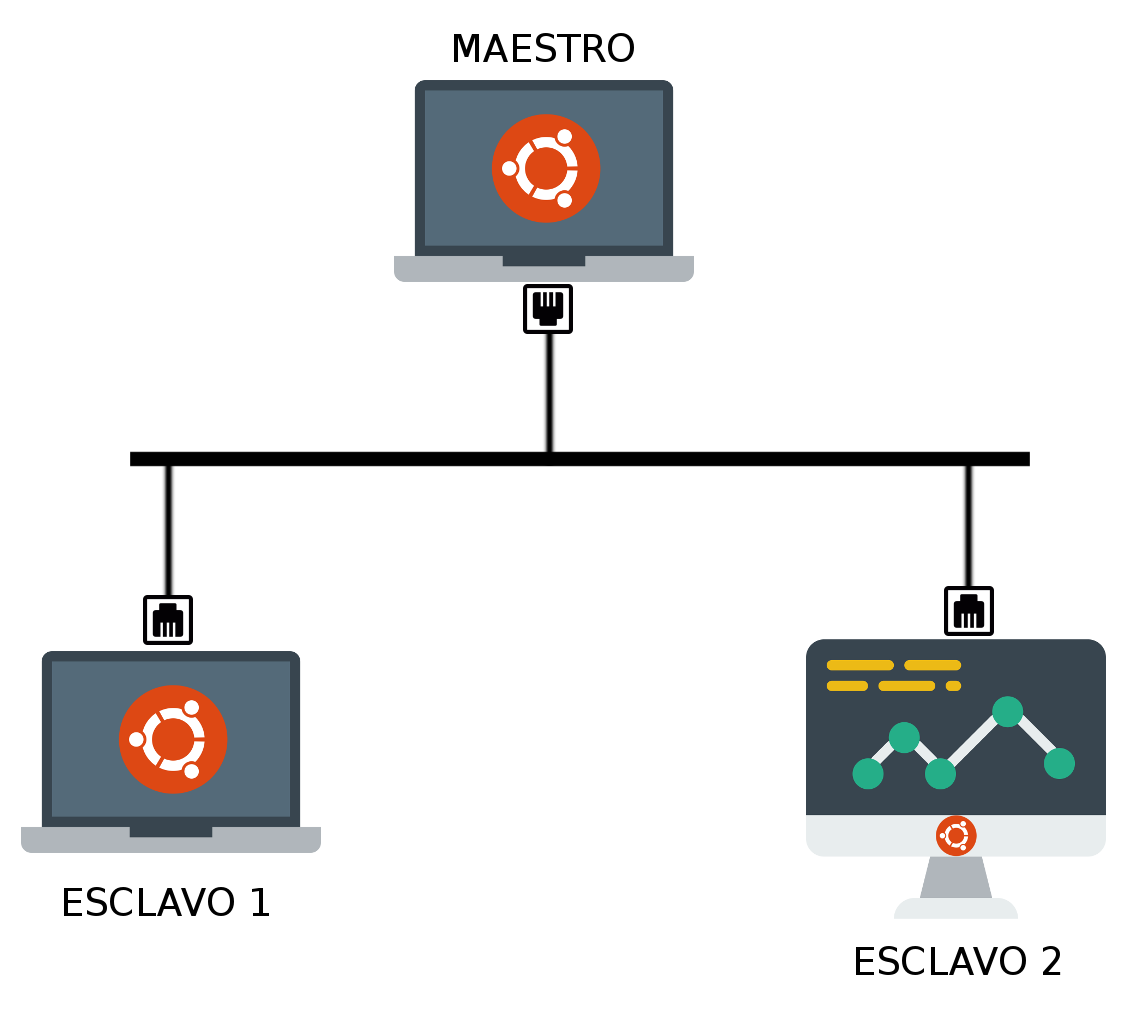
\includegraphics[scale=0.3]{graphics/clusterDomestico}
\end{figure}

\textit{Apache Hadoop} es la tecnología utilizada para montar este mecanismo de replicación mediante el uso de su sistema distribuido de ficheros (\gls{HDFS}) que resulta óptimo para esta configuración. Este mecanismo nos permitirá tener los datos en cada nodo del clúster y, así, lo único que circulará por la red serán las tareas que el maestro asigne a los esclavos y los resultados que estos obtengan tras su procesamiento. 

Esto evitará el tráfico que generaría transmitir los datos a procesar con la tarea asignada a los nodos esclavos, mejorando el rendimiento de la arquitectura.

\begin{figure}[htp!]
	\centering
	\caption{Esquema del sistema de replicación \gls{HDFS}}
	\label{fig:hdfs}
	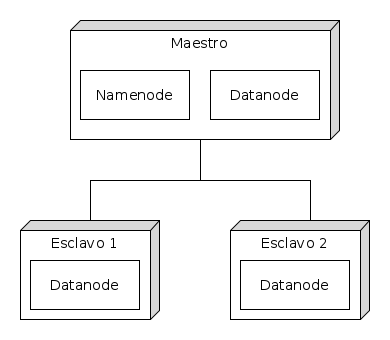
\includegraphics[scale=0.6]{graphics/hadoop}
\end{figure}

Como se aprecia en la figura \ref{fig:hdfs} que muestra el esquema del sistema de replicación, para su funcionamiento, en cada nodo se necesita un proceso \textit{datanode} ejecutándose, que será el que se encargue de el almacenamiento de los datos en la máquina. Además, para controlar el estado de los \textit{datanodes} se necesita un proceso \textit{namenode}, que se ejecutará en el nodo maestro.

\clearpage
\section{Insights del proyecto \label{insights}}
En este trabajo debido a que se realiza un proyecto real de análisis para una supuesta empresa de impartición de cursos, hay ciertas preguntas que se desean resolver a lo largo del proyecto, estás ``preguntas'' en ámbito de \textit{big data} se denominan \textit{insights} que iremos resolviendo hasta llegar al informe final.

\begin{itemize}
	\item ¿Cuáles son los lenguajes de programación más populares?
	\item En caso de regionalización ¿Qué países enfocar?
	\item ¿Qué idioma utilizan los programadores?
\end{itemize}

El primer paso para enfrentarnos a estos \textit{insights} será definir el termino ``popularidad'', para luego proceder a la resolución de estas cuestiones.


\subsection{Plan de proyecto}
El proyecto constará de diferentes fases donde primero implementaremos el clúster anteriormente mencionado.
Realizando un pequeño estudio preliminar encontramos que los programadores utilizan tres plataformas de forma predominante.
\begin{itemize}
 	\item \textbf{Stackoverflow \cite{stackoverflow}}. Esta plataforma está dedicada a que los programadores planteen dudas, que son resueltas por otro profesionales. Cada \textit{post} esta etiquetado con el lenguaje o tecnología sobre la que se realiza la cuestión.
 	
 	\item \textbf{GitHub \cite{github}}. Es un repositorio de versiones basado en \textit{Git} \cite{git}, el cual siguiendo la filosofía de \textit{open data} \cite{opendata} proporciona una \gls{API} desde la que se pueden descargar los eventos almacenados desde 2015 a través de \textit{GitHub Archive} \cite{githubArchive}.
 	
 	\item \textbf{Twitter \cite{twitter}}. Es una plataforma de comunicación bidireccional con naturaleza de red social (porque permite elegir con quien te relacionas). Cuyos mensajes están limitados a 280 caracteres. Aquí los usuarios publican sus opiniones personales o anuncios que consideran importantes. Proporciona una \gls{API} que permite obtener estos mensajes (\textit{tweets}) en tiempo real.
\end{itemize}



%
% Instalación del clúster
%
\chapter{Instalación del clúster \label{sec:implementacion}}

\section{Introducción}
En este apartado se detallarán los aspectos relevantes para la implementación de la arquitectura \textit{big data} diseñada en el apartado \ref{sec:disenho}.

Como se indica en dicho apartado, se plantean una configuracion para el sistema multinodo, donde una máquina es el maestro y, el resto, los esclavos.

Por tanto, se comentaran todos los detalles y pasos para montar la arquitectura diseñada y, de esta forma, conseguir un sistema \textit{big data} funcional y completo que sea capaz de almacenar, procesar y analizar los datos para obtener las respuestas de las consultas planteadas.

\section{Preparación del entorno de trabajo}
Como se expuso en el apartado \ref{sparkEA}, donde se habla de \textit{Apache Spark}, este, resulta compatible con las tres sistemas operativos más importantes para ordenadores, aunque la solución escogida ha sido Linux para ejecutarlo. Se va a utilizar Ubuntu Desktop \cite{ubuntu} para el master y Ubuntu Server para los slaves. 

Aunque se podría ejecutar todo el clúster exclusivamente en un entorno Ubuntu Server, se ha decidido utilizar la variante Desktop en el master para poder realizar los análisis directamente desde el nodo.

\subsection{Especificaciones del equipo \label{eqEspec}}
\begin{table}[htp!]
	\centering
	\caption{Especificaciones del maestro}
	\label{maestro}
	\begin{tabular}{|l|l|}
		\hline
		\multicolumn{2}{|c|}{\textbf{GENERAL}}                                 \\ \hline
		\textbf{Nombre:}            & david-hdp		                           \\ \hline
		\textbf{Sistema Operativo:} & Linux                                    \\ \hline
		\textbf{Versión:}           & Ubuntu 16.10 (64 bits)                   \\ \hline
		\textbf{Usuario:}           & david                         	       \\ \hline
		\multicolumn{2}{|c|}{\textbf{SISTEMA}}                                 \\ \hline
		\textbf{Procesador:}        & Intel(R) Core(TM) i7-3820 CPU @ 4.30GHz  \\ \hline
		\textbf{Cores:}             & 8                                        \\ \hline
		\textbf{Threads por core:}  & 2                                        \\ \hline
		\textbf{RAM:}               & 16384                                    \\ \hline
		\multicolumn{2}{|c|}{\textbf{ALMACENAMIENTO}}                          \\ \hline
		\textbf{Dispositivo:}       & Kingston SUV400S37480G                   \\ \hline
		\textbf{Tamaño:}            & 1 Tb	                                   \\ \hline
		\multicolumn{2}{|c|}{\textbf{RED}}                                     \\ \hline
		\textbf{Dispositivo:}       & Realtek PCIe GBE Family Controller       \\ \hline
		\textbf{Nombre:}            & Master                                   \\ \hline
	\end{tabular}
\end{table}

\begin{table}[htp!]
	\centering
	\caption{Especificaciones del nodo1}
	\label{esclavo}
	\begin{tabular}{|l|l|}
		\hline
		\multicolumn{2}{|c|}{\textbf{GENERAL}}                             			    \\ \hline
		\textbf{Nombre:}            & node1			                         			\\ \hline
		\textbf{Sistema Operativo:} & Linux                                   			\\ \hline
		\textbf{Versión:}           & Ubuntu 16.10 (64 bits)                   			\\ \hline
		\textbf{Usuario:}           & david                         	       			\\ \hline
		\multicolumn{2}{|c|}{\textbf{SISTEMA}}                                 			\\ \hline
		\textbf{Procesador:}        & Intel(R) Celeron(TM) T1600 @ 2GHz  	\\ \hline
		\textbf{Cores:}             & 2                                        			\\ \hline
		\textbf{Threads por core:}  & 1                                        			\\ \hline
		\textbf{RAM:}               & 	8192                                    			\\ \hline
		\multicolumn{2}{|c|}{\textbf{ALMACENAMIENTO}}                          			\\ \hline
		\textbf{Dispositivo:}       & Samsung HM320JI\\ \hline
		\textbf{Tamaño:}            & 320 Gb	                                   			\\ \hline
		\multicolumn{2}{|c|}{\textbf{RED}}                                     			\\ \hline
		\textbf{Dispositivo:}       & Realtek PCIe GBE Family Controller       			\\ \hline
		\textbf{Nombre:}            & node1                                  			\\ \hline
	\end{tabular}
\end{table}

\clearpage
\subsection{Instalación del sistema operativo}
Esta instalación solo fue necesaria de llevar a cabo en los esclavos que utilizaríamos para el entorno doméstico. Como se ha comentado anteriormente, el \gls{SO} elegido será Ubuntu, concretamente, la versión 16.10.

\subsubsection{Requisitos previos}
Para proceder con la instalación del sistema operativo en los ordenadores había que cumplir algunos requisitos muy básicos. Lo primero era contar con máquinas que superasen los requisitos mínimos \cite{ubuntu} necesarios para su correcta ejecución, cosa que las utilizadas cumplían (especificaciones en el apartado \ref{eqEspec}). 


También sería necesario un soporte de instalación del \gls{SO}, que en este caso fue un \gls{DVD}), en el que se grabó una imagen con Ubuntu, que permitió el inicio de este sistema operativo en las máquinas y su posterior instalación en ellas, de forma local en el disco duro.

\subsection{Instalación de Apache Spark}
Para la realización de este proyecto utilizaremos la versión 2.2.0 \textit{Apache Spark}, que era la versión disponible cuando se comenzó a trabajar en él. Como lo que se deseaba era una versión estable para realizar todo el trabajo, se descartó la creación del paquete a partir del código fuente y, también, la actualización a la versión 2.2.1 que salió en diciembre. 

Por tanto, para la instalación de \textit{Apache Spark} en los equipos que se utilizarían se recurrió a la versión pre-compilada del \Gls{framework} \cite{descargaSpark}, en concreto la compilada para funcionar con \textit{Apache Hadoop 2.9} que se utilizaría en la configuración multinodo del clúster.


\subsubsection{Prerrequisitos}
Para que \textit{Apache Spark} funcione de forma correcta en el sistema se necesita cumplir una serie de prerrequisitos:

\begin{itemize}
	\item Tener instalado Linux en el sistema.
	\item Tener instalado Java en el sistema.
	\item Tener instalado Scala \cite{scala} en el sistema.
	\item Tener instalado Python en el sistema.
	\item Tener instalado SSH en el sistema.
	\item Disponer de un usuario y grupo común en todas las máquinas.
\end{itemize}


\subsubsection{Instalación de Java y Scala}
La instalación de estos dos lenguajes es esencial para el funcionamiento de \textit{Apache Spark} debido a que está escrito en Scala. Por otro lado, Java es necesario ya que Scala \cite{scala} necesita de la \gls{JVM} para su funcionamiento.

La instalación de estos dos lenguajes de programación se realiza a través de la terminal de forma muy sencilla, primero se añade el repositorio oficial de Oracle \cite{descargaJava} y posteriormente se introduce los comandos de instalación.
Los comandos necesarios se encuentran en el bloque de código \ref{ins:java}.

\begin{lstlisting}[label=ins:java,language=sh,frame=single, caption=Instalación de Java y Scala.]
sudo add-apt-repository ppa:webupd8team/java
sudo apt-get update
sudo apt-get install oracle-java8-installer
sudo apt install scala
\end{lstlisting}

\subsubsection{Instalación de Anaconda (Python)}
Python va a ser esencial para el desarrollo de este proyecto ya que se utilizará la \gls{API} en este lenguaje para escribir todo el código que procese \textit{Apache Spark}, conocida como \textit{PySpark}. Además como \gls{IDLE} utilizaremos \textit{Jupyter Notebook} \cite{jupyter}, que es ampliamente conocido en el entorno de la ciencia de datos.

Para instalar tanto Python como \textit{Jupyter Notebook} vamos a utilizar una distribución, que contiene estos y además muchas otras librerías útiles, llamada \textit{Anaconda} \cite{anaconda}. La instalación se realizara en la carpeta \textit{``/opt''} del sistema.
Los comandos necesarios para la instalación se encuentran en el bloque de código \ref{ins:anaconda}.

\begin{lstlisting}[label=ins:anaconda,language=sh,frame=single, caption=Descarga e instalación de Anaconda.]
sudo wget https://repo.continuum.io/archive/Anaconda3-5.0.1-Linux-x86_64.sh
sudo bash Anaconda3-5.0.1-Linux-x86_64.sh
\end{lstlisting}

\subsubsection{Creación de usuario y grupo común \label{grupoComun}}
Para evitar posibles problemas de permisos durante la ejecución de las tareas, es buena práctica tener un grupo de usuarios donde estén las máquinas incluidas en el clúster.

Por tanto, para abordar este problema, durante la instalación del \gls{SO} en las máquinas del clúster se estableció el mismo nombre de usuario para todas. Además, tras esta se creo un nuevo grupo de usuarios, donde se incluyó a dichos usuarios. El proceso para la creación del grupo y adición del usuario a este se puede encontrar en el fragmento de código \ref{usuarioGru}

\clearpage
\begin{lstlisting}[label=usuarioGru,language=sh,frame=single,caption=Creación de grupo común y adición del usuario del sistema a este.]
sudo addgroup spark
sudo adduser --ingroup spark david
\end{lstlisting}

Una vez realizados estos pasos, las máquinas de la red tendrían acceso a los ficheros de cualquier otra si el grupo tuviese permisos de acceso en dichos archivos. En este caso, todo el conjunto de ficheros utilizados por el sistema \textit{big data} tendrá acceso de lectura y escritura por el grupo de usuarios \textit{spark}, como se explicará en la configuración de \textit{Apache Spark}.

\subsubsection{Instalación de \gls{SSH} y creación del certificado \label{insSSH}}
El cliente de \gls{SSH} viene instalado por defecto en Ubuntu y Debian, sin embargo, para que los nodos devuelvan la llamada del maestro y establecer la conexión cuando se inicie el clúster, será necesario que estos dispongan del servidor \gls{SSH}. 

Estos programas también se encuentran en el repositorio oficial de Ubuntu, por lo que la instalación se realiza escribiendo el nombre del paquete en la terminal. Con respecto a los equipos de la universidad, estos están ya instalados para su uso. El comando de consola para instalarlo se encuentra en el fragmento de código \ref{ins:ssh}.

\begin{lstlisting}[label=ins:ssh,language=sh,frame=single,caption=Instalación del cliente y el servidor de \gls{SSH}.]
sudo apt install openssh-client
sudo apt install openssh-server
\end{lstlisting}

Una vez instalados los programas, el siguiente paso será crear el certificado \gls{SSH} para cada equipo y, así, facilitar las conexiones entre los nodos. Es decir, una vez creado los certificados \gls{SSH} de cada máquina, si estos son compartidos entre ellas, los equipos pasarán a estar en la lista de dispositivos seguros y no será necesaria la autentificación con contraseña para establecer la conexión.

El proceso de creación de certificados se puede encontrar en el fragmento de código \ref{confCert} y se realizará en todos las máquinas.

\begin{lstlisting}[label=confCert,language=sh,frame=single,caption=Creación y autorización del certificado \gls{SSH}.]
ssh-keygen -t rsa -P ""
cat $HOME/.ssh/id_rsa.pub >> $HOME/.ssh/authorized_keys
\end{lstlisting}

Tras estos pasos, ya tenemos los prerrequisitos completos para iniciar la instalación del clúster.

\clearpage
\subsubsection{Instalación y configuración del modo distribuido}
Este apartado se tratará la configuración de \textit{Apache Spark} para la configuración distribuida o multinodo, donde existe una máquina que hará de maestro y $n$ máquinas que harán de esclavos. 

\paragraph{Asignación de IPs y nombres de sistema en la red.}
Este proceso se realizará para simplificar la conexión entre los nodos de los sistemas utilizados, permitiendo con ellos, realizar las conexiones \gls{SSH} mediante el uso de los nombres asignados, en vez de las direcciones  
IP locales.

En este caso se realizará modificando el archivo ``/etc/hosts'' en cada nodo utilizado. Como se tenemos dos equipos el \textit{master} recibirá el nombre de ``david-hdp'' que es el nombre que tenía anteriormente y el esclavo será \textit{nodo n} donde $n$ será su número de esclavo en el sistema. La modificación del archivo ``hosts'' será la misma para todos los nodos, añadiendo las líneas que se encuentran en el fragmento de código \ref{confhosts}

\begin{lstlisting}[label=confhosts,language=sh,frame=single,caption=Líneas a añadir en el fichero ``/etc/hosts'' de cada nodo del clúster.]
192.168.1.15 	david-hdp
192.168.1.17	node1
\end{lstlisting}

\paragraph{Compartición de certificados \gls{SSH}.}
Como se indicó en el apartado \ref{insSSH}, la creación de los certificados \gls{SSH} permitirá que, al compartirse entre los equipos que formen el clúster, no sea necesaria la autentificación con contraseña, simplificando el proceso de conexión entre las máquinas. Además este proceso es requerido tanto por \textit{Apache Spark} como por \textit{Apache Hadoop} para realizar la interoperatividad.

En el caso del entorno doméstico, será el maestro el que necesite los certificados de los esclavos para realizar la conexión, por lo que el proceso seguido es la copia de estos en el nodo maestro. El proceso inverso y la compartición entre esclavos no será necesaria, ya que, es el maestro el que inicia la conexión y porque los esclavos no están conectados entre sí.

Es exclusivamente el maestro el que requiere certificarse en los esclavos para realizar la conexión, por lo que el proceso seguido es la copia de estos en el nodo maestro. El proceso inverso y la adición entre esclavos no será necesaria, ya que, es el maestro el que inicia la conexión y los esclavos no están interconectados.

Los comandos a ejecutar en la terminal del nodo maestro para la obtención de los certificados de los esclavos se puede encontrar en el fragmento de código \ref{comandosSSH}.

\begin{lstlisting}[label=comandosSSH,language=sh,frame=single,caption=Obtención de los certificados \gls{SSH} de los esclavos por parte del maestro en el clúster.]
ssh-copy-id -i $HOME/.ssh/id_rsa.pub david@node1
\end{lstlisting}

Por último, para evitar que el servidor \gls{SSH} rechace las peticiones de forma automática editaremos el fichero ``/etc/ssh/sshd\_config'', la modificación será reflejada en el fragmento de código \ref{confsshd}.

\begin{lstlisting}[label=confsshd,language=sh,frame=single,caption=Líneas modificadas en el fichero ``/etc/ssh/sshd\_config'' cada nodo del clúster.]
PasswordAuthentication No
\end{lstlisting}

Posteriormente para hacer efectivo el cambio se ejecutará el comando que se puede encontrar en el fragmento de código \ref{sshdrestart} o simplemente reiniciando el equipo.

\begin{lstlisting}[label=sshdrestart,language=sh,frame=single,caption=Comando de consola para reiniciar el servidor \gls{SSH}.]
sudo service sshd restart
\end{lstlisting}

\paragraph{Instalación de \textit{Apache Spark}.}
La instalación de \textit{Apache Spark} en este caso se tiene que hacer de forma manual en cada máquina del sistema,
Para la realización de este proceso de forma automática en cada nodo se creó un script que se ejecutaría en cada nodo del sistema \textit{big data}. El código de este se puede encontrar en el fragmento de código \ref{insSpark}.

\begin{lstlisting}[label=insSpark,language=sh,frame=single,caption=Script de instalación de \textit{Apache Spark}.]
#!/bin/bash
cd /opt
wget http://apache.uvigo.es/spark/spark-2.2.0/spark-2.2.0-bin-hadoop2.7.tgz
tar -xvzf spark-2.2.0-bin-hadoop2.7.tgz 
mv spark-2.2.0-bin-hadoop2.7 spark
rm -rf spark-2.2.0-bin-hadoop2.7.tgz
chmod 1777 -R /opt/spark
\end{lstlisting}

\paragraph{Configuración de \textit{Apache Spark}.}
El primer paso a realizar es indicar al sistema la ruta de instalación de \textit{Apache Spark} y de Java, modificando el archivo ``.bashrc'' de cada nodo. Debido a que el nombre de usuario es el mismo en todos los equipos, el fragmento de código a añadir en el fichero es el mismo para todos, siendo este el que se puede encontrar en el código \ref{confBash}. Se puede ver el fichero ``.bashrc'' completo en el anexo \ref{sc:bashrc}.

Por otro lado, también hay que modificar los archivos de configuración de \textit{Apache Spark} para su correcto funcionamiento los cuales se pueden encontrar en ``/opt/spark/conf''. Primero se modificará el archivo ``spark-env.sh'' en todos los nodos, para establecer que máquina será la maestra y donde se ha instalado java y python. Estas últimas líneas no serían necesarias, dado que debería haberse añadido esta variable de sistema durante la instalación de java.
\clearpage
\begin{lstlisting}[label=confBash,language=sh,frame=single,caption=Líneas a añadir en el fichero ``spark-env.sh'' para configurar \textit{Apache Spark} en el modo distribuido.]
export SPARK_MASTER_IP=david-hdp # Nombre del maestro del cluster
export JAVA_HOME=/usr/lib/jvm/java-8-oracle
export HADOOP_CONF_DIR=/opt/hadoop/etc/hadoop

export SPARK_WORKER_INSTANCES=1
export SPARK_DRIVER_MEMORY=2G
export PYSPARK_PYTHON=/opt/anaconda3/bin/python3.6
export PYSPARK_DRIVER_PYTHON=/opt/anaconda3/bin/python3.6
\end{lstlisting}

Por último, a partir de la versión 2.0 de \textit{Apache Spark} las configuraciones genéricas ya no se realizan en el fichero ``spark-env.sh'' sino en el fichero ``spark-defaults.conf'', en nuestro caso el contenido de dicho fichero es el especificado en el fragmento de código \ref{sparkDefaults}.

\begin{lstlisting}[label=sparkDefaults,language=sh,frame=single,caption=Contenido del fichero ``spark-defaults.conf'' de configuración de \textit{Apache Spark}.]
spark.master                     spark://david-hdp:7077
spark.eventLog.dir               hdfs:///spark-history
spark.eventLog.enabled           true
spark.history.fs.logDirectory    hdfs:///spark-history
spark.history.provider           org.apache.spark.deploy.history.FsHistoryProvider
spark.history.ui.port            18080
spark.executor.memory            2G
spark.executor.cores             2
\end{lstlisting}

Tras realizar esto, el siguiente paso, será establecer que máquinas de la red formarán parte del clúster. Esto se indicará en el archivo  ``/opt/spark/conf/slaves'', donde se escribirá el nombre de red de los nodos que se utilizarán. En este caso, al ser el maestro también un esclavo se le incluirá en dicho fichero, en un clúster de producción el maestro no sería en ningún caso esclavo, es más, existirían dos maestros para prevenir la caída de uno de ellos. Las líneas a añadir en el fichero se puede encontrar en el fragmento de código \ref{slaves} que solo será necesario escribir en el nodo maestro, que será el que realice las conexiones.

\begin{lstlisting}[label=slaves,language=sh,frame=single,caption=Líneas a añadir en el fichero ``slaves'' para establecer las máquinas a utilizar en el clúster.]
localhost # Es la maquina maestra
node1
\end{lstlisting}

\clearpage
\subsection{Configuración de \textit{Jupyter Notebook}}
Como se ha comentado anteriormente en la sección \ref{jupyterEA} se va a utilizar como \gls{IDLE} \textit{Jupyter Notebook}. Para poder utilizar PySpark en \textit{Jupyter} se ha de crear un nuevo kernel, para ello ser hará uso del código \ref{jupyterfile} y se escribirán las líneas reflejadas en el fragmento \ref{jupyterKernel}. 

\begin{lstlisting}[label=jupyterfile,language=sh,frame=single,caption=Comando para generar el kernel \textit{Jupyter} para PySpark.]
sudo mkdir -p /opt/anaconda3/share/jupyter/kernels/pyspark
sudo nano /opt/anaconda3/share/jupyter/kernels/pyspark/kernel.json
\end{lstlisting}

\begin{lstlisting}[label=jupyterKernel,frame=single,caption=Contenido del fichero ``kernel.json'' para la configuración con \textit{Apache Spark}.]
{
	"display_name": "PySpark",
	"language": "python",
	"argv": [
		"/opt/anaconda3/bin/python3",
		"-m",
		"ipykernel",
		"-f",
		"{connection_file}"
	],
	"env": {
		"SPARK_HOME": "/opt/spark/",
		"PYTHONPATH": "/opt/spark/python:/opt/spark/python/lib/py4j-0.10.4-src.zip",
		"PYTHONSTARTUP": "/opt/spark/python/pyspark/shell.py"
	}
}
\end{lstlisting}

La variable asociada al ``pythonpath'' del fragmento \ref{jupyterKernel} puede variar según la versión de \textit{Apache Spark} por lo que sería necesario comprobar si corresponde a la instalada. En este caso, debido a la versión que hemos utilizado la numeración del fichero es la correcta.

\clearpage
\subsection{Instalación de \textit{Apache Hadoop}\label{hadoopCluster}}

Como se ha indicado en el diseño de la arquitectura \textit{big data}, en el apartado \ref{sec:disenho}, para la configuración distribuida del clúster se necesita un mecanismo de replicación de datos para su funcionamiento. Por tanto, como se explicó, se decidió usar \textit{Apache Hadoop}, en concreto su sistema de ficheros distribuido, \gls{HDFS}, que permitirá la disponibilidad de las trazas en todos los nodos del clúster.

En este apartado se va a proceder a explicar el proceso de instalación y configuración de este sistema. La versión de \textit{Apache Hadoop} utilizada en este proyecto es la versión 2.9.0 precompilada, que está disponible para su descarga desde la página oficial \cite{descargaHadoop}.

Al tratarse de un sistema distribuido, al igual que con la instalación de \textit{Apache Spark}, esta deberá realizarse en cada sistema. Para agilizar este proceso, se ha creado un script para que realice la descarga del fichero ``.tar.gz'', lo descomprima y lo mueva a la ubicación seleccionada para su instalación. Esta ubicación será similar a la de \textit{Apache Spark}, es decir, será instalado en la ruta ``/opt/hadoop/''. El script ejecutado se encuentra en el fragmento de código \ref{insHadoop}.


\begin{lstlisting}[label=insHadoop,language=sh,frame=single,caption=Script de instalación de \textit{Apache Hadoop}.]
#!/bin/bash
wget http://www-us.apache.org/dist/hadoop/common/stable2/hadoop-2.9.0.tar.gz
tar -xzvf hadoop-2.9.0.tar.gz
mv hadoop-2.9.0/ /opt/hadoop
rm -rf hadoop-2.9.0.tar.gz
chmod 1777 -R /opt/hadoop
\end{lstlisting}

\paragraph{Estructura de carpetas para \textit{Apache Hadoop}.} Antes de iniciar la configuración de de \textit{Apache Hadoop} vamos a crear la estructura de directorios de trabajos de \gls{HDFS} que configuraremos posteriormente. Como se ha explicado anteriormente en la sección \ref{hadoopEA}, existen dos tipos de nodo, \textit{datanode} y \textit{namenode}, el primero contiene los datos de replicación y no existe limitación en cuanto a su número, mientras el segundo tipo es un nodo de control o nodo maestro. 

Esta diferencia es importante ya que se van a realizar dos estructuras diferentes según el tipo de nodo. Para el nodo maestro vamos a realizar la estructura que aparece reflejada en la figura \ref{fig:estructMaster}, los comandos para su realización se pueden ver en el fragmento de código \ref{cod:estructMaster}.

\begin{figure}[htp!] 
	\centering		
	\caption{Estructura de carpetas para operativa del \textit{namenode}.}
	\label{fig:estructMaster}
	\vspace{5pt}
	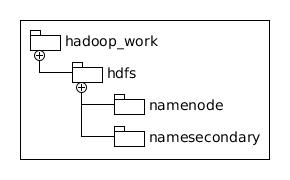
\includegraphics[scale=0.8]{graphics/estructMaster}
\end{figure}

\begin{lstlisting}[label=cod:estructMaster,language=sh,frame=single,caption=Codigo de creación de la estructura de carpetas del \textit{namenode}.]
sudo mkdir -p /opt/hadoop_work/hdfs/namenode
sudo mkdir -p /opt/hadoop_work/hdfs/namesecondary
\end{lstlisting}

Para los nodos esclavos se va a realizar la estructura de carpetas reflejada en la figura \ref{fig:estructSlave}. Para la realización de este proceso de forma automática en cada nodo se creó un script que se ejecutaría en cada nodo del sistema \textit{big data}. El código de este se puede encontrar en el fragmento de código \ref{cod:estructSlave}.

\begin{figure}[htp!] 
	\centering		
	\caption{Estructura de carpetas para operativa del \textit{datanode}.}
	\label{fig:estructSlave}
	\vspace{5pt}
	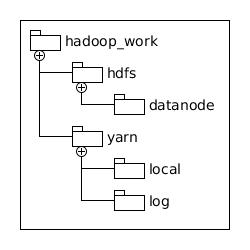
\includegraphics[scale=0.8]{graphics/estructSlave}
\end{figure}

\begin{lstlisting}[label=cod:estructSlave,language=sh,frame=single,caption=Codigo de creación de la estructura de carpetas del \textit{datanode}.]
#!/bin/bash
mkdir -p /opt/hadoop_work/hdfs/datanode
mkdir -p /opt/hadoop_work/yarn/local
mkdir -p /opt/hadoop_work/yarn/log
chown david:david -R /opt/hadoop_work/
\end{lstlisting}

\clearpage
\paragraph{Configuración de \textit{Apache Hadoop.}}
Tras la descarga e instalación de \textit{Apache Hadoop}, para su funcionamiento, será necesario modificar diferentes archivos de configuración. Lo primero será modificar los archivos de sistema para establecer correctamente las rutas de instalación y, posteriormente, los ficheros propios del \gls{framework}.

Como en el caso de la instalación de \textit{Apache Spark} el fichero de sistema a modificar es ``bashrc'', al que habrá que añadirle unas líneas indicando diferentes rutas de instalación de los módulos de \textit{Apache Hadoop} para su funcionamiento. Las lineas a añadir se pueden encontrar en el fragmento de código \ref{bashadoop}.

\begin{lstlisting}[label=bashadoop,language=sh,frame=single,caption=Líneas a añadir a ``.bashrc'' para el funcionamiento de \textit{Apache Hadoop}.]
export HADOOP_HOME=/opt/hadoop
export PATH=$PATH:$HADOOP_HOME/bin
export PATH=$PATH:$HADOOP_HOME/sbin
export HADOOP_CONF_DIR=$HADOOP_HOME/etc/hadoop
export HADOOP_MAPRED_HOME=$HADOOP_HOME
export HADOOP_COMMON_HOME=$HADOOP_HOME
export HADOOP_HDFS_HOME=$HADOOP_HOME
export HADOOP_YARN_HOME=$HADOOP_HOME
export YARN_HOME=$HADOOP_HOME
export HADOOP_COMMON_LIB_NATIVE=$HADOOP_HOME/lib/native
export HADOOP_OPTS="-Djava.library.path=$HADOOP_HOME/lib"
export CLASSPATH=$CLASSPATH:$HADOOP_HOME/lib/*
\end{lstlisting}

Posteriormente, se modificarán los diferentes ficheros de configuración de \textit{Apache Hadoop} para hacerlo funcionar en el clúster doméstico. Todos estos archivos residen en la ruta ``/opt/etc/hadoop''. Los ficheros a modificar serán los siguientes:

\begin{itemize}
\item \textbf{hadoop-env.sh:} Donde se indicará la ruta de instalación de Java en la máquina.
\begin{lstlisting}[label=hadoopenv,language=sh,frame=single,caption=Línea a añadir a ``hadoop-env.sh''.]
export JAVA\_HOME=/usr/lib/jvm/java-8-oracle
\end{lstlisting}

\item \textbf{core-site.xml}
\begin{lstlisting}[label=coresite,language=XML,frame=single,caption=Contenido del ``core-site.xml''.]
<configuration>
	<property>
		<name>fs.defaultFS</name>
		<value>hdfs://david-hdp:9000</value>
	</property>
	
	<property>
		<name>ipc.maximum.data.length</name>
		<value>134217728</value>
	</property>
	<property>
		<name>io.file.buffer.size</name>
		<value>131072</value>
	</property>
</configuration>
\end{lstlisting}

\item \textbf{hdfs-site.xml}
\begin{lstlisting}[label=hdfssite1,language=XML,frame=single,caption=Contenido del ``hdfs-site.xml'' de el nodo maestro.]
<configuration>
	<property>
		<name>dfs.replication</name>
		<value>2</value>
		<description>Replication factor, 1 no copy, 2 two copies each fragment</description> 
	</property>
	<property>
		<name>dfs.namenode.name.dir</name>
		<value>file:/opt/hadoop_work/hdfs/namenode</value>
		<description>Carpeta correspondiente al NameNode</description> 
	</property>
	<property>
		<name>dfs.datanode.data.dir</name>
		<value>file:/opt/hadoop_work/hdfs/datanode</value>
		<description>Carpeta correspondiente al DataNode</description> 
	</property>
	<property>
		<name>dfs.namenode.checkpoint.dir</name>
		<value>file:/opt/hadoop_work/hdfs/namesecondary</value>
		<description>Carpeta correspondiente al NameSecondary</description> 
	</property>
	<property>
		<name>dfs.block.size</name>
		<value>134217728</value>
		<description>Tamanno maximo de bloque de archivo (128Mb)</description> 
	</property>
	<property>
		<name>dfs.webhdfs.enabled</name>
		<value>true</value>
	</property>
</configuration>
\end{lstlisting}

\clearpage
\begin{lstlisting}[label=hdfssite2,language=XML,frame=single,caption=Contenido del ``hdfs-site.xml'' de los nodos esclavos.]
<configuration>
	<property>
		<name>dfs.replication</name>
		<value>2</value>
		<description>Replication factor, 1 no copy, 2 two copies each fragment</description> 
	</property>
	<property>
		<name>dfs.datanode.data.dir</name>
		<value>file:/opt/hadoop_work/hdfs/datanode</value>
		<description>Carpeta correspondiente al DataNode</description> 
	</property>
	<property>
		<name>dfs.namenode.checkpoint.dir</name>
		<value>file:/opt/hadoop_work/hdfs/namesecondary</value>
		<description>Carpeta correspondiente al NameSecondary</description> 
	</property>
	<property>
		<name>dfs.block.size</name>
		<value>134217728</value>
		<description>Tamanno maximo de bloque de archivo (128Mb)</description> 
	</property>
</configuration>
\end{lstlisting}

\item \textbf{ mapred-site.xml}
\begin{lstlisting}[label=mapredsite,language=XML,frame=single,caption=Contenido del ``mapred-site.xml''.]
<configuration>
	<property>
		<name>mapreduce.framework.name</name>
		<value>yarn</value>
	</property>
	<property>
		<name>mapreduce.jobhistory.address</name>
		<value>david-hdp:10020</value>
		<description>Direccion de acceso al historial</description>
	</property>
	<property>
		<name>mapreduce.jobhistory.webapp.address</name>
		<value>david-hdp:19888</value>
		<description>Acceso a la app web</description>
	</property>
	<property>
		<name>jobtracker.thrift.address</name>
		<value>0.0.0.0:9290</value>
		<description>Block size</description>
	</property>
	<property>
		<name>mapred.jobtracker.plugins</name>
		<value>org.apache.hadoop.thriftfs.ThriftJobTrackerPlugin</value>
		<description>Comma-separated list of jobtracker plug-ins to be activated.</description>
	</property>
</configuration>
\end{lstlisting}

\item \textbf{ yarn-site.xml}
\begin{lstlisting}[label=yarnsite,language=XML,frame=single,caption=Contenido del ``yarn-site.xml''.]
<configuration>
	<property>
		<name>yarn.resourcemanager.hostname </name>
		<value>david-hdp</value>
	</property>
	<property>
		<name>yarn.resourcemanager.bind-host</name>
		<value>0.0.0.0</value>
	</property>
	<property>
		<name>yarn.nodemanager.bind-host</name>
		<value>0.0.0.0</value>
	</property>
	<property>
		<name>yarn.nodemanager.aux-services</name>
		<value>mapreduce_shuffle</value>
	</property>
	<property>
		<name>yarn.nodemanager.auxservices.mapreduce.shuffle.class</name>
		<value>org.apache.hadoop.mapred.ShuffleHandler</value>
	</property>
	<property>
		<name>yarn.log-aggregation-enable</name>
		<value>true</value>
	</property>
	<property>
		<name>yarn.nodemanager.local-dirs</name>
		<value>file:/opt/hadoop_work/yarn/local</value>
	</property>
	<property>
		<name>yarn.nodemanager.log-dirs</name>
		<value>file:/opt/hadoop_work/yarn/logs</value>
	</property>
	<property>
		<name>yarn.nodemanager.remote-app-log-dir</name>
		<value>hdfs://david-hdp:9000/var/log/hadoop-yarn/apps</value>
		<description>logs en hdfs</description>
	</property>
</configuration>
\end{lstlisting}

\item \textbf{master:} Máquina en la que resida el \textit{namenode}.
\begin{lstlisting}[label=masterHadoop,language=sh,frame=single,caption=Línea a añadir a ``master''.]
david-hdp
\end{lstlisting}

\item \textbf{slaves:} Máquinas en la que resida el \textit{datanode}, es decir, donde se repliquen los datos.
\begin{lstlisting}[label=slavesHadoop,language=sh,frame=single,caption=Líneas a añadir a ``slaves''.]
david-hdp
node1
\end{lstlisting}
\end{itemize}

\clearpage
\subsection{Instalación de \textit{Apache Flume}}
Al tratarse de un sistema distribuido, al igual que con la instalación de \textit{Apache Spark}, esta deberá realizarse en cada sistema. Como en los casos anteriores se utilizará una versión precompliada de \textit{Apache Flume} que puede encontrarse en la página de descarga oficial \cite{descargaFlume}

Para agilizar este proceso, se ha creado un script para que realice la descarga del fichero ``.tar.gz'', lo descomprima y lo mueva a la ubicación seleccionada para su instalación. Esta ubicación será similar a la de \textit{Apache Spark}, es decir, será instalado en la ruta ``/opt/flume/''. El script ejecutado se encuentra en el fragmento de código \ref{insFlume}.

\begin{lstlisting}[label=insFlume,language=sh,frame=single,caption=Script de instalación de \textit{Apache Flume}.]
#!/bin/bash

wget http://apache.rediris.es/flume/1.8.0/apache-flume-1.8.0-bin.tar.gz
tar -xzvf apache-flume-1.8.0-bin.tar.gz
mv apache-flume-1.8.0-bin/ /opt/flume
rm -rf apache-flume-1.8.0-bin.tar.gz
chmod 1777 -R /opt/flume
\end{lstlisting}

\paragraph{Configuración de \textit{Apache Flume.}} Además se deberá editar el fichero de configuración de \textit{Apache Flume} para indicarle la localización de la instalación de java, para ello se modificará el fichero en la ruta ``/opt/flume/conf/flume-env.sh'' como se encuentra en el fragmento de código \ref{flumeenv}.

\begin{lstlisting}[label=flumeenv,language=sh,frame=single,caption=Línea a añadir a ``flume-env.sh''.]
export JAVA\_HOME=/usr/lib/jvm/java-8-oracle
export JAVA_OPTS="-Xms2000m -Xmx10000m -Dcom.sun.management.jmxremote"
\end{lstlisting}

\section{Arranque y parada del clúster}
Con todos los pasos anteriores realizados correctamente necesitamos iniciar el clúster, para ello se realizará con una serie de comandos iniciando cada parte de forma independiente. Para automatizar este proceso se han creado dos scripts de arranque y parada, se puede ver el código de estos scripts en las figuras \ref{cod:startServer} para el inicio y en la figura \ref{cod:stopServer} la parada del mismo.

\begin{lstlisting}[label=cod:startServer,language=sh,frame=single,caption=Script de inicio del clúster implementado.]
#!/bin/bash
printf "\n\nLaunching Hadoop"
printf "\n--------------------------\n\n"
printf "\nStarting DFS system:\n"
$HADOOP_HOME/sbin/start-dfs.sh
printf "\nStarting yarn daemons"
$HADOOP_HOME/sbin/start-yarn.sh
printf "\nStarting mapreduce history"
$HADOOP_HOME/sbin/mr-jobhistory-daemon.sh start historyserver

printf "\n\nLaunching Apache Spark"
printf "\n--------------------------\n\n"
$SPARK_HOME/sbin/start-all.sh
printf "\n\nLaunching Apache Spark History Server"
$SPARK_HOME/sbin/start-history-server.sh
\end{lstlisting}

\begin{lstlisting}[label=cod:stopServer,language=sh,frame=single,caption=Script de parada del clúster implementado.]
#!/bin/bash
printf "\n\nStoping Hadoop"
printf "\n--------------------------\n\n"
printf "\nStoping DFS system"
$HADOOP_HOME/sbin/stop-dfs.sh
printf "\nStoping yarn daemons"
$HADOOP_HOME/sbin/stop-yarn.sh
printf "\nStoping mapreduce history server"
$HADOOP_HOME/sbin/mr-jobhistory-daemon.sh stop historyserver

printf "\n\nStoping Apache Spark"
printf "\n--------------------------\n\n"
$SPARK_HOME/sbin/stop-all.sh
printf "\n\nStoping Apache Spark History Server"
$SPARK_HOME/sbin/stop-history-server.sh
\end{lstlisting}

Una vez iniciado el clúster se deben generar las carpetas y ficheros que formarán parte del mismo, esto lo hace \textit{Apache Hadoop} de forma automática utilizando el comando \ref{hadoopFormat} y posteriormente se debe crear la carpeta del usuario que se realiza con el segundo comando del fragmento \ref{hadoopFormat}

\begin{lstlisting}[label=hadoopFormat,language=sh,frame=single,caption=Comandos requeridos en la primera ejecución del clúster.]
hadoop namenode -format
hdfs dfs -mkdir -p /user/david	
\end{lstlisting}

%
% Fase de StackOverflow
%
\chapter{Stack Overflow \label{sec:stackoverflow}}

\section{Introducción}
Empezó en 2008 por \textit{Joel Spolsky} con su blog \textit{``Coding Horror''} con la idea de crear un sitio de preguntas y respuestas. Un año más tarde con la ayuda de \textit{Jeff Atwood} apareció el sitio conocido como \textit{Stack Overflow} \cite{stackoverflow} donde los especialista de \gls{IT} pueden plantear sus dudas y ser respondidos por otros profesionales del sector.

Esta plataforma ha ido evolucionando rápidamente desde sus inicios hasta convertirse en una web de referencia, como es actualmente, para los profesionales del sector.

\section{Aprovisionamiento de datos}

La empresa propietaria de la web \textit{Stack Overflow} \cite{stackoverflow}, \textit{Stack Exchange} \cite{stackexchange}, siguiendo la cultura de \textit{open data} \cite{opendata} hace públicos los datos relacionados con sus comunidades entre las que se encuentra la que vamos a analizar para este proyecto.

Estos datos se encuentra publicados en la web de \textit{Stack Exchange Data Dump} \cite{stofData}, distribuidos libremente bajo licencia \textit{Creative Commons} \cite{creativecommons}. Para este proyecto vamos a descargar exclusivamente los ficheros relacionados, que son los que se pueden ver en la figura \ref{stof:bruteFiles}

\clearpage
\begin{lstlisting}[label=stof:bruteFiles,frame=single,caption=Ficheros públicos sobre \textit{Stack Overflow} en la web de \textit{Data Dump}.]
stackoverflow.com-Badges.7z           			  180.9M
stackoverflow.com-Comments.7z         			  3.4G
stackoverflow.com-PostHistory.7z      			  19.7G
stackoverflow.com-PostLinks.7z        			  62.8M
stackoverflow.com-Posts.7z            			  11.3G
stackoverflow.com-Tags.7z             			  709.2K
stackoverflow.com-Users.7z            			  328.0M
stackoverflow.com-Votes.7z            			  826.8M
\end{lstlisting}

Estos archivos vienen comprimidos en 7z \cite{7z}, por lo tanto, el primer paso es descomprimirlos, dicho proceso se completa en un tiempo total de 4 horas. Los ficheros descomprimidos están en formato \gls{XML}, al abrirlos comprobamos que la estructura de estos ficheros consiste en un elemento por etiqueta. Dado \textit{Apache Spark} no permite de forma nativa la lectura de este tipo de ficheros, se deberá crear un script que realice la conversión de formato.

\section{Procesado de datos}
Los datos vienen en \gls{XML} \cite{XML}, un formato no soportado de forma nativa en \textit{Apache Spark} por lo que el primer paso es convertir estos datos en uno soportado como es \gls{JSON}. Se ha creado un script llamado ``xml2json.py'' que hará esta labor.

La primera parte del script son los \textit{imports} necesarios que se pueden apreciar en el fragmento de código \ref{stof:xml2jsonImport}, donde se pueden ver tres principales:
\begin{itemize}
	\item \textbf{OS:} Será utilizado para comprobar la existencia de los ficheros de entrada y salida.
	\item \textbf{json:} Utilizado para generar las cadenas de texto resultantes del proceso.
	\item \textbf{lxml:} Librería que realizara el \textit{parseo} para la extracción de los datos necesarios del \gls{XML}.
\end{itemize}
\begin{lstlisting}[label=stof:xml2jsonImport,language=Python,frame=single,caption=\textit{Imports} del script ``xml2json.py'' de procesado de \gls{XML}., firstnumber=1,numbers=left]
#!/usr/bin/env python3.6

"""
Este programa solo extrae los atributos de cada elemento,
y ademas da por hecho que cada elemento esta alojado en una unica linea
Usage: 
./xml2json.py  inputFile outputFile
./xml2json.py /opt/Posts.xml /opt/Posts.json
"""
import sys
import json
import tqdm # Solo para ver como avanza
from time import time
from hurry.filesize import size
from os import path, remove
from lxml import etree
\end{lstlisting}

Se realiza la comprobación sobre la existencia del fichero de entrada, en caso afirmativo el script continua y en caso contrario se informa al usuario y termina la ejecución del mismo. Posteriormente se comprueba la existencia del fichero de salido, en caso de que este exista se le informa al usuario preguntándole si desea sobreescribirlo, ejecutando las acciones necesarias según la decisión de este. Esta parte se puede ver en el fragmento de código \ref{stof:xml2jsonCheck}.

\begin{lstlisting}[label=stof:xml2jsonCheck,language=Python,frame=single,caption=Fragmento de código del script ``xml2json.py'' de comprobación del estado de los ficheros \textit{in/out}., firstnumber=24,numbers=left]
# Se comprueba si el fichero de entrada existe
if path.isfile(_input) == False:
	print('El fichero no existe')
	sys.exit() # Si no existe se interrumpe la ejecucion

# Se comprueba si el fichero de salida existe
# Si existe, se le pregunta al usuario si desea sobreescribirlo
if path.isfile(_output):
	isOverwrite = input('El fichero {} ya existe, Desea sobreescribirlo?[Y/n]: '.format(_output))
	if isOverwrite.lower() == 'y':
		remove(_output)	
\end{lstlisting}

En el fragmento de código \ref{stof:xml2jsonSave} se declara una función encargada de la persistencia del \gls{JSON}. Aunque la la librería ``lxml'' retorna un diccionario, este no es de tipo básico de python y por tanto la librería ``json'' no es capaz de procesarlo, para solucionar este inconveniente se recorre la lista de pares clave-valor y se almacenan consecutivamente en un diccionario de tipo básico. Por último se abre el fichero de destino en modo \textit{``append''} y se guardan los \gls{JSON} resultantes del proceso.

\begin{lstlisting}[label=stof:xml2jsonSave,language=Python,frame=single,caption=Fragmento de código del script ``xml2json.py'' encargado de la persistencia de resultados., firstnumber=36,numbers=left]
# Metodo para guardar los atributos en json
def save_json(atributos, count):
	# Se convierten los atributos (etree.Attrib) a tipo diccionario
	dict_json = dict()
	for k,v in atributos.items():
		dict_json[k]=v
	# Se convierte el diccionario en un .json y se le agrega un salto de linea final
	str_json = json.dumps(dict_json) + '\n'
	# Se abre el fichero en modo 'append' y se escribe el .json
	with open(_output, 'a') as f:
		f.write(str_json)
\end{lstlisting}

La función principal (fragmento de código \ref{stof:xml2jsonMain} del script consiste en abrir el fichero de entrada en modo lectura y comenzar a leer línea a línea. Cada línea es procesada y guardada antes de continuar con la siguiente.

Cada línea leída es convertida en un nodo de tipo árbol por la librería ``lxml'' y de cada nodo se extraen sus atributos. Por si dicho nodo perteneciese a una etiqueta que no deseemos, como es la etiqueta de definición, se comprueba que esta posea el atributo ``Id'' entre ellos; si todo es correcto se llama al método \textit{``save\_json''} para su almacenamiento. La función principal del script corresponde al fragmento de código \ref{stof:xml2jsonMain}.

\begin{lstlisting}[label=stof:xml2jsonMain,language=Python,frame=single,caption=Fragmento de código del script ``xml2json.py'' encargado de la persistencia de resultados., firstnumber=48,numbers=left]
# Se abre el fichero de entrada
with open(_input, 'r') as f:
	#Creamos un progress bar donde el total de proceso es el tamano del fichero
	progress = tqdm.tqdm(unit='bytes', leave=False,total=path.getsize(_input), \
	bar_format="{l_bar}{bar}| {percentage:3.0f}% [{elapsed}<{remaining}, {rate_fmt}{postfix}]")
	# Se va leyendo linea a linea
	for line in f:
		# Se va actualizando la barra con el tamano en bytes de la linea leida.
		progress.update(sys.getsizeof(line)) 
		try:
			node = etree.fromstring(line) 	# Se convierte el texto en un arbol
			atributos = node.attrib 		# Se obtinen los atributos
			if atributos.has_key('Id'):	
				save_json(atributos, count)
			count+=1
		except Exception as f: # Algunas lineas como la descripcion de formato dan error
			print(line)
	progress.close()
\end{lstlisting}

\clearpage
\section{Análisis de datos}
La fase de análisis de datos consiste en documentar el valor de los datos, asegurar su calidad y veracidad. Para este estadio no es necesario usar el total de los datos, pues ello supondría mucho tiempo de procesado, a tal efecto se coge una muestra pequeña, pero significativa, de cada origen. En este caso los ficheros mencionados al inicio de la sección.

El primer paso realizado es la obtención de un esquema de estructura de datos de cada fichero, la cual se puede apreciar en la figura \ref{stof:fullschema}

\begin{figure}[htp!] 
	\centering		
	\caption{Esquema completo de \textit{Stack Overflow}.}
	\label{stof:fullschema}
	\vspace{5pt}
	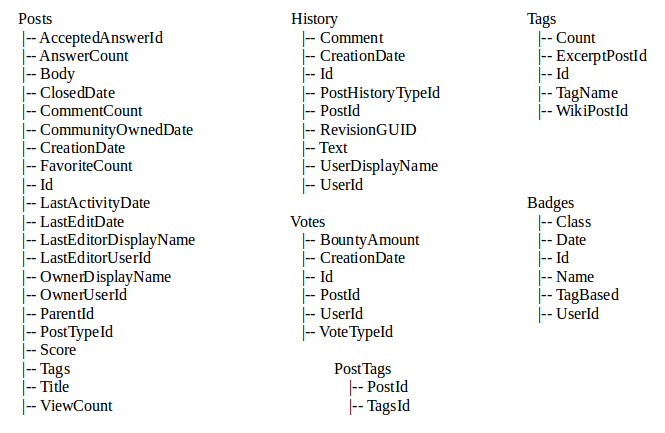
\includegraphics[scale=0.68]{graphics/schema-stack} 
\end{figure}

Llegados a este punto deberemos establecer que datos serán los que utilicemos y qué valor poseen estos. El primer problema al que nos enfrentemos será definir el término ``popularidad''; para ello nos encontramos con varias formas de resolverlo: qué pregunta recibe más votos, cuál recibe más \textit{badges}, cuál es el más visitado, sobre cuál se crean más \textit{posts}, en cuál comenta más gente, etc...

Realizando un pequeño análisis descubrimos varias cosas:
\begin{itemize}
	\item No tenemos información sobre le número de visitas.
	\item Los tipos de votos son demasiado dispares para definir un valor exacto de cada en relación al \textit{tag}.
	\item Los \textit{badges} varían a lo largo del tiempo, asignándose más a principios y finales de año, debido a la naturaleza de los mismos.
	\item Los comentarios no indican el interés absoluto de los profesionales del sector, unicamente la capacidad, conocimiento o participación de los usuarios activos.
	\item Los \textit{posts} se crean cuando los usuarios tienen una duda no resuelta anteriormente o cuando la duda no se resuelve fácilmente.
\end{itemize}

Este sencillo análisis deja solamente una opción dirigida directamente a resolver los \textit{insights} establecidos, los \textit{posts}.

Una vez que hemos decidido que serán los \textit{posts} quienes no  van a proporcionar los datos necesarios para resolver la popularidad, continuaermos analizando cuáles de estos datos serán los más relevantes. 

Los datos que a \textit{priori} consideramos más relevantes son el \textit{tag}, el \textit{creationDate} y el \textit{score}. Además, para obtener el \textit{tag} de cada \textit{post}, deberemos cruzarlos con la tabla de \textit{tags} a través de \textit{PostTags}, que nos permitirán conocer que lenguaje o tecnología pertenece cada \textit{posts}.

Realizaremos una primera consulta a través del módulo de \textit{Spark SQL} y almaceno los resultados. En el fragmento de código \ref{stof:anaTopSQL} podemos ver como se realiza una consulta a través de este módulo. Pero de momento la consulta \gls{SQL} usada para la relación se puede observar en fragmento de código \ref{stof:sql1}.

% Escribir código 
\begin{lstlisting}[label=stof:sql1,language=sql,frame=single,caption={Consulta \gls{SQL} para la extraccion de la fecha, \textit{tag} y \textit{score} de las consultas en \textit{Stack Overflow}.}]
SELECT t.tag,
	date_format(creation_date, '%Y-%m) AS month,
	COUNT(*) AS count,
	SUM(q.score) AS score
FROM posts p
INNER JOIN tags t on p.id = t.id
WHERE score > 0
GROUP BY month, t.tag;
\end{lstlisting}

La consulta del código \ref{stof:sql1} nos devolverá la puntuación que le han dado los usuarios ordenada por mes y lenguaje, almacenamos los datos, para análisis futuros. A partir de estos datos, podemos realizar la búsqueda de los lenguajes más populares.

Establecemos una búsqueda de los lenguajes atendiendo al número de apariciones de los lenguajes en el último año, a través de \textit{Spark SQL}.
Estas consultas son gestionadas por el \textit{Spark Core}. Para empezar a trabajar con \textit{Apache Spark} debemos declarar algunas variables importantes como son el \textit{SparkContext} o el \textit{SparkSession}.

En primer lugar, realizaremos los \textit{imports} y la inicialización tanto de \textit{SparkContext}, como del \textit{SparkSession} tal y como se puede apreciar en el fragmento de código \ref{stof:anaImport}, esto será común a todos los scripts de \textit{Apache Spark} por lo que se evitará repetir código a lo largo del proyecto.

\begin{lstlisting}[label=stof:anaImport,language=Python,frame=single,caption=\textit{Imports} y configuración de una sessión de \textit{Apache Spark}.]
from pyspark import SparkConf, SparkContext
from pyspark.sql.functions import col, asc, desc
from pyspark.sql.types import StructType, StructField, StringType, IntegerType

conf = SparkConf().setAppName("Jupyter: Stack Posts")
conf = conf.setMaster("spark://david-hdp:7077")
sc = SparkContext(conf=conf)
spark = SparkSession(sc)
\end{lstlisting}

Dado que los resultados del código \ref{stof:sql1} se han exportado a un \gls{CSV} sin cabecera, deberemos crear un \textit{schema} de manera manual, para ello \textit{Apache Spark} proporciona unos tipos de datos propios para relacionas los \textit{schemas} con su origen de datos. Como se puede observar en el código \ref{stof:anaSchema}, se ha creado un \textit{schema} de cuatro campos.

\begin{lstlisting}[label=stof:anaSchema,language=Python,frame=single,caption=Código de declaración del \textit{schema} para lectura del \gls{CSV}.]
schema = StructType([
	StructField("tag", StringType(), True),
	StructField("fecha", StringType(), True),
	StructField("count", IntegerType(), True),
	StructField("score", IntegerType(), True),
	StructField("answers", IntegerType(), True)])
\end{lstlisting}

El siguiente paso será importar el fichero que contiene los datos indicandole el \textit{schema} del fragmento de código \ref{stof:anaSchema} y lo guardamos en una variable llamada ``df'' de la forma que aparecen el código \ref{stof:anaDF} y posteriormente se visualiza una muestra de los datos para comprobar como están almacenados los datos. Esta muestra se puede ver en la tabla \ref{stof:dfTable} donde vemos los $6$ primeros elementos del \textit{dataframe}.

\begin{lstlisting}[label=stof:anaDF,language=Python,frame=single,caption=Carga de un fichero \gls{CSV} con un esquema predefinido con el módulo \textit{Spark \gls{SQL}}.]
df = spark.read.csv('stof/clean/mysql_clean.csv', schema=schema)
\end{lstlisting}

\begin{table}[htp!]
	\centering
	\caption{\textit{DataFrame} de muestra de datos de \textit{Stack Overflow}.}
	\label{stof:dfTable}
	\begin{tabular}{@{}|r|r|r|r|r|@{}}
		\hline
		\textbf{tag}  & \textbf{fecha}   & \textbf{count} & \textbf{score} & \textbf{answers} \\ \hline
		.net & 2010-03 & 1073  & 6385  & 2768    \\
		.net & 2011-02 & 1036  & 4408  & 2101    \\
		.net & 2011-03 & 1030  & 5493  & 2192    \\
		.net & 2010-08 & 1018  & 5003  & 2443    \\
		.net & 2011-05 & 1004  & 4015  & 1906    \\
		.net & 2011-04 & 987   & 3718  & 1977    \\ 
		\hline
	\end{tabular}
\end{table}

Una vez que tengamos los datos cargados, ya se puede empezar a trabajar con ellos. El primer hito a resolver son los lenguajes más populares. Para ello vamos a realizar una consulta \gls{SQL} que nos devuelva los diez primeros lenguajes y/o tecnologías más populares del último año. El primer paso será generar una tabla temporal para poder operar con \gls{SQL}, dicha función la cumple la primera línea del fragmento de código \ref{stof:anaTopSQL}.

\begin{lstlisting}[label=stof:anaTopSQL,language=Python,frame=single,caption=Código de generación de la tabla temporal y la ejecución de una consulta \gls{SQL}.]
# Nueva tabla temporal
df.createOrReplaceTempView("temp_talble")

# Ejecucion de consulta SQL
top10 = spark.sql("\
	SELECT tag, \
		SUM(count) AS count, \
		SUM(score) AS score\
	FROM temp_table \
	WHERE \
		fecha >= "2016-12" \
	GROUP BY tag \
	ORDER BY count DESC \
	LIMIT 10")
\end{lstlisting}

El resultado de esta consulta se muestra en la tabla \ref{stof:anaTop}, esta es la lista de las diez tecnologías más populares o, dicho de otra manera, sobre qué tecnologías están preguntando los profesionales del sector de \gls{IT}. 

\begin{table}[htp!]
	\centering
	\caption{Tabla con los 10 lenguajes más populares de \textit{Stack Overflow}.}
	\label{stof:anaTop}
	\begin{tabular}{|r|r|r|}
		\hline
		\multicolumn{1}{|c|}{\textbf{tag}} & \multicolumn{1}{c|}{\textbf{count}} & \multicolumn{1}{c|}{\textbf{score}} \\ \hline
		javascript                         & 482970                              & 876320                              \\
		c\#                                & 436792                              & 810352                              \\
		java                               & 354105                              & 644255                              \\
		android                            & 352392                              & 720040                              \\
		python                             & 267364                              & 498320                              \\
		c++                                & 232816                              & 677424                              \\
		php                                & 213584                              & 328408                              \\
		ios                                & 181032                              & 383838                              \\
		c                                  & 91936                               & 219344                              \\
		\multicolumn{1}{|r|}{html}         & \multicolumn{1}{c|}{91788}          & \multicolumn{1}{c|}{163830}         \\ \hline
	\end{tabular}
\end{table}

Con estos datos se puede iniciar el aprovisionamiento de datos en twitter utilizando estos resultados como \textit{keywords}.

 
%
% Fase de Twitter
%
\chapter{Twitter \label{sec:twitter}}

\section{Introducción}
Twitter \cite{twitter} es una plataforma de comunicación bidireccional con naturaleza de red social (porque permite elegir con quien te relacionas). Cuyos mensajes están limitados a 280 caracteres. Aquí los usuarios publican sus opiniones personales o anuncios que consideran importantes. Proporciona una \gls{API} que permite obtener estos mensajes (\textit{tweets}) en tiempo real.

La idea nación en 1992, en la mente de \textit{Jack Dorsey}, inspirada en el \textit{software} de rastreo de los taxistas. Finalmente el proyecto se concretó en 2006 como un servicio interno entre los empleados de \textit{Odeo} y fue lanzado exitosamente en 2007 gracias a la popularidad de los \textit{smartphones}

Hoy día Twitter es uno de los sistemas de comunicación más utilizados, no solo para información intrascendente, social, sino como herramienta de comunicación entre profesionales.

\clearpage
\section{Aprovisionamiento de datos}
Para realizar el aprovisionamiento de datos en Twitter, el primer movimiento consiste en informarse sobre la \gls{API} de Twitter \cite{apiTwitter}, rápidamente se puede observar que ofrece tres niveles de acceso: al archivo completo, a los datos de la última semana y a los datos en tiempo real. Debido a que los dos primeros niveles requieren reuniones, pago y aprobación por parte de la empresa, vamos a utilizar los datos en tiempo real.

La captación de \textit{tweets} en tiempo real y su ingesta en \gls{HDFS} se va a realizar a través de \textit{Apache Flume}, para ello se va a configurar un agente que nos permita obtenerlos y almacenarlos en \gls{HDFS}.

\subsection{Agente de \textit{Apache Flume}}
Para este caso específico \textit{Cloudera} \cite{cloudera} proporciona una librería de java que permite obtener los \textit{tweets} en formato \gls{JSON}, lo que simplificará enormemente el análisis y el filtrado de datos.

El agente de \textit{Apache Flume} está completo en el código \ref{flumeAgent}, se definen el origen (\textit{source}), el canal (\textit{channel}) y el sumidero de datos (\textit{sink}), la primera parte de la configuración corresponde a Twitter, donde se deberán indicar las cuatro claves que proporciona el \gls{API} del mismo y los \textit{keywords} que se desean obtener, los cuales han sido obtenidos anteriormente en el análisis de \textit{Stack Overflow} y aparecen en la tabla \ref{stof:anaTop}.

La siguiente parte del código corresponde al sumidero o \textit{sink}, en inglés, donde se le indica que los datos se mantienen en memoria y que se almacenan en \gls{HDFS}, también se especifican los datos necesarios para la conexión con el clúster de \textit{Apache Hadoop}; así como datos más específicos dependientes de la configuración del clúster.

\begin{lstlisting}[label=flumeAgent,language=make,frame=single,caption=Fichero de configuración del agente de \textit{Apache Flume} para \textit{Twitter}.]
TwitterAgent.sources = Twitter
TwitterAgent.channels = MemChannel
TwitterAgent.sinks = HDFS

TwitterAgent.sources.Twitter.type = com.cloudera.flume.source.TwitterSource
TwitterAgent.sources.Twitter.channels = MemChannel
TwitterAgent.sources.Twitter.consumerKey = <ConsumerKey>
TwitterAgent.sources.Twitter.consumerSecret = <ConsumerSecret>
TwitterAgent.sources.Twitter.accessToken = <AccessToken>
TwitterAgent.sources.Twitter.accessTokenSecret = <AccessTokenSecret>
TwitterAgent.sources.Twitter.keywords = javascript, androiddev , python , c++ , php , iosdev , html, kotlin, php, typescript, powershell, git, github, groovy, maven, cplusplus, springboot, haskell, androidstudio, intellij, netbeans, oracle, mysql, cprograming, c#


TwitterAgent.sinks.HDFS.channel = MemChannel
TwitterAgent.sinks.HDFS.type = hdfs
TwitterAgent.sinks.HDFS.hdfs.path = hdfs://david-hdp:9000/user/david/flume/tweets/%Y-%m-%d/
TwitterAgent.sinks.HDFS.hdfs.fileType = DataStream
TwitterAgent.sinks.HDFS.hdfs.writeFormat = Text
TwitterAgent.sinks.HDFS.hdfs.batchSize = 100
TwitterAgent.sinks.HDFS.hdfs.rollSize = 100000
TwitterAgent.sinks.HDFS.hdfs.rollCount = 10000

TwitterAgent.channels.MemChannel.type = memory
TwitterAgent.channels.MemChannel.capacity = 10000
TwitterAgent.channels.MemChannel.transactionCapacity = 100
\end{lstlisting}

\paragraph{Lanzamiento del agente.} Para el inicio del agente de \textit{Apache Flume} se utiliza el comando del código \ref{launchFlume} y se deja funcionar en segundo plano para que se vayan almacenando una cantidad significativa de \textit{tweets}.

\begin{lstlisting}[label=launchFlume,language=sh,frame=single,caption=Comando de lanzamiento del agente de \textit{Apache Flume} para \textit{Twitter}.]
flume-ng agent --conf /opt/flume/conf --conf-file /home/david/scripts/Flume-TwitterAgent.conf
\end{lstlisting}

\section{Análisis de datos}
Para el análisis de datos se configurará una sesión de \textit{Apache Spark} como se ha indicado en el código \ref{stof:anaImport} y cargar los datos del aprovisionamiento de Twitter, la primera parte consiste en identificar el \textit{schema} para visualizar la estructura de los datos proporcionados por Twitter. La estructura completa está compuesta por un total de $1241$ campos, puede verse en el apéndice \ref{sc:tweet}, aquí se muestra un pequeño extracto en el fragmento de código \ref{tw:struct}.

\begin{lstlisting}[label=tw:struct,frame=single,caption=Extracto del esquema de un \textit{tweet}.]
|-- created_at: string (nullable = true)
|-- geo: struct (nullable = true)
|    |-- coordinates: array (nullable = true)
|    |    |-- element: double (containsNull = true)
|    |-- type: string (nullable = true)
|-- lang: string (nullable = true)
|-- place: struct (nullable = true)
|    |-- country: string (nullable = true)
|    |-- country_code: string (nullable = true)
|    |-- full_name: string (nullable = true)
|    |-- id: string (nullable = true)
|    |-- name: string (nullable = true)
|    |-- place_type: string (nullable = true)
|    |-- url: string (nullable = true)
|-- text: string (nullable = true)
\end{lstlisting}

Para resolver algunos de los \textit{insights} planteados en la sección \ref{insights}, en este caso aprovecharemos los datos que proporciona Twitter sobre el idioma en el que esta escrito un \textit{tweet}, así como la ubicación desde la que se emite el mismo.

Tras un periodo de análisis de los campos existentes se descubren varios hechos:
\begin{itemize}
	\item Existe un campo llamado \textit{``geo''} el cual corresponde a un campo antiguo (\textit{deprecated}), el cual ya no debería estar en uso, por tanto se descarta para precisar la ubicación.
	
	\item Una estructura llamada \textit{``place''} que proporciona varios campos referentes a la ubicación del usuario, cuyo dato se rige por la \gls{ISO} 3166-1 alpha-2 \cite{isogeo}.

	\item \textit{``created\_at''} proporciona la fecha de creación del \textit{tweet} en cuestión, aunque para este análisis no resultará relevante.
	
	\item El campo \textit{``lang''} indica el idioma en el que está escrito el \textit{tweet}, bajo la normativa de estandarización \gls{ISO} 639-1:2002 \cite{isolang}.
\end{itemize}

Con esto en mente vamos a realizar un script en \textit{Apache Spark} que nos permita extraer estos datos y almacenarlos. En un clúster más grande y para una empresa \textit{data driven} estos datos se filtrarían de una forma menor para futuros análisis, es más, prácticamente no recibirían ninguna transformación.

\clearpage
\section{Procesado de datos}

\subsection{Script Apache Spark}
Como en casos anteriores, se declaran las variables necesarias y se inicia una sesión de \textit{Apache Spark} y se cargan los datos (ver código \ref{stof:anaImport}). Por motivos de espacio en el clúster se filtrará periódicamente y se almacenará el resultado en \gls{HDFS}.
\begin{lstlisting}[label=tw:sql,language=sql,frame=single,caption={Consulta \gls{SQL} para la extraccion de datos de Twitter}.]
SELECT 
	lang,
	place.country_code,
	text
FROM
	tweets
WHERE
	place IS NOT NULL;
\end{lstlisting}

Se realiza el filtrado con la consulta \gls{SQL} que aparece en el código \ref{tw:sql} de la forma ya mostrada en el código \ref{stof:anaTopSQL}. Esta consulta extraerá el país, el lenguaje que se menciona en el \textit{tweet} y el idioma en el que está escrito. El segundo filtro comprueba que aparezca alguno mencionado, y esto es debido a que la \gls{API} de Twitter no filtra las palabras por contenido literal, sino por relación.

Por último se almacenan los resultados en HDFS para su posterior uso, este resultado se graba en una carpeta con múltiples archivos. Para simplificar el contenido y por utilizarlo en la generación de un mapa posterior, se creará un \gls{CSV}, pero no es posible añadirle cabecera al fichero, por tanto para resolver esto y automatizar el proceso se creará un pequeño script \textit{bash}.

\subsection{Script Bash para normalizar resultados}
El script tiene la función principal de unir todos los ficheros generados por el proceso anterior y darle una cabecera al fichero \gls{CSV}.

Este contiene muchos comandos que están explicados en el código \ref{tw:bash1}, además se realizan dos extracciones, una con los ficheros que contienen datos de geolocalización y otra sin ellos. No existe variación en los comandos a excepción de la cabecera asignada y la estructura de carpetas.

\begin{lstlisting}[label=tw:bash1,language=sh,frame=single,caption=Comandos utilizados durante el proceso de unificación de datos., firstnumber=1,numbers=left]
#!/bin/bash
# Comrpueba si existe el fichero (0) o si no existe (1)
check_nongeo="hdfs dfs -test -e twitter/single/nongeo.tweets.csv"
# Crea un csv con todos los datos de la carpeta twitter/nongeo/*
create_nongeo="hdfs dfs -getmerge twitter/nongeo/* nongeo.csv"
# Agrega cada linea del fichero nongeo.csv al fichero nongeo.tweets.csv
merge_nongeo_local="cat nongeo.csv >> nongeo.tweets.csv"
# Suma el fichero 'nongeo.csv' del local al 'twitter/single/nongeo.tweets.csv' del hdfs
merge_nongeo_dfs="hdfs dfs -appendToFile nongeo.csv twitter/single/nongeo.tweets.csv"
# Sube el fichero a hdfs
upload_nongeo="hdfs dfs -put nongeo.tweets.csv twitter/single/"
\end{lstlisting}

La segunda fase de este script consiste en comprobar si este proceso se ha realizado anteriormente y en caso afirmativo ya no sería necesario construir una cabecera, tan solo sería necesario agregar los nuevos registros al fichero existente. Dado que este proceso requiere un tiempo se han agregado varias salidas por pantalla para mantener al usuario informado del desarrollo del script. Esta segunda fase se puede ver en el fragmento de código \ref{tw:bash2}.

\begin{lstlisting}[label=tw:bash2,language=sh,frame=single,caption=Código bash de evaluación. , firstnumber=40,numbers=left]
echo "Evaluando fichero geo"
if [ '$exist_geo' == '1' ]; then
	echo "No existe fichero ../geo.tweets.csv"
	echo "Creando cabecera de csv"
	echo 'lang, country, text' > geo.tweets.csv
	echo "Exportando datos del hdfs"
	eval $create_geo
	echo "Creando fichero local con cabecera"
	eval $merge_geo_local
	echo "Subiendo fichero ../geo.tweets.csv"
	eval $upload_geo
	echo "fichero ../geo.tweets.csv subido"
	echo "Eliminando ficheros geo auxiliares..."
	eval $remove_geo_local
	eval $remove_geo_tweets
	echo "Ficheros auxilaires geo, eliminados!"
else
	echo "Existe el fichero ../geo.tweets.csv"
	echo "Exportando datos del hdfs"
	eval $create_geo
	echo "Uniendo fichero local con hdfs"
	eval $merge_geo_dfs
	echo "Eliminando fichero geo auxiliar..."
	eval $remove_geo_local
	echo "Fichero geo auxiliar, eliminado!"
fi
\end{lstlisting}

%
% Fase de GitHub
%
\chapter{GitHub \label{sec:github}}

\section{Introducción}
GitHub es un repositorio de versiones basado en \textit{Git} \cite{git}, el cual siguiendo la filosofía de \textit{open data} \cite{opendata} proporciona una \gls{API} desde la que se pueden descargar los eventos almacenados desde 2015 a través de \textit{GitHub Archive} \cite{githubArchive}.

Nacido en 2008 en una oficina del Valle de San Francisco (como tantos otros proyectos), GitHub tiene hoy más de 9 millones de usuarios registrados, más de 200 millones de visitas al mes y ha sido valorado en más de 2000 millones de dólares (por lo que está en la Unicorn List \cite{unicornList} de Fortune). Utilizan GitHub para gestionar y almacenar su código desde Google a la Casa Blanca pasando por Facebook o incluso el Ayuntamiento de Madrid \cite{gitAytoMad}.

\clearpage
\section{Análisis de datos}
Para el análisis de datos se configurará una sesión de \textit{Apache Spark} como se ha indicado en el código \ref{stof:anaImport} y cargaremos una pequeña muestra de datos. El aprovisionamiento de datos se explicará más adelante.

La primera parte consiste en identificar el \textit{schema} para visualizar la estructura de los datos proporcionados por GitHub. La estructura completa está compuesta por un total de $752$ campos, esta se puede consultar en el apéndice \ref{sc:github}.

Lo ideal sería obtener los \textit{commits} diarios de cada lenguaje. Para ello analizamos los 38 tipos de eventos \cite{gitEvents} que proporciona la \gls{API} de GitHub. Como resultado se decide que el evento que vamos a utilizar como medida de referencia va a ser el ``PushEvent'', el cual contiene los \textit{commits} realizados por los usuarios de la plataforma.

Se observa que dicho evento efectivamente proporciona el número de \textit{commits} realizados por un usuario, así como la fecha y hora en la que se realiza pero, no aporta ningún dato referente al lenguaje que contiene dicho \textit{commit}.

Para obtener los lenguajes se evalúa la posibilidad de utilizar la \gls{API} para realizar la solicitud del lenguaje correspondiente al repositorio sobre el que se realiza el \textit{commit}. En una primera revisión de dicha \gls{API} visualizamos que existe un límite de peticiones de la misma, siendo esta de $60$ solicitudes por hora para usuarios no identificados y en caso de identificarse el límite sube apenas a $5000$. Teniendo en cuenta el volumen de los datos se descarta esta opción.

Por todo ello se decide realizar un segundo análisis de la estructura para intentar identificar si existe la posibilidad de extraer estos datos de otro tipo de evento. En el transcurso de la misma se identifican dos eventos que proporcionan la información del lenguaje identificado en el repositorio, estos eventos son ``PullRequestReviewCommentEvent'' y ``PullRequestEvent''.

Como resultado de lo comentado anteriormente se decide generar dos conjuntos de datos, uno con las fechas, número e \textit{id} del repositorio sobre el que se realiza el commit y otro con el \textit{id} y los lenguajes asociados al mismo, para posteriormente cruzar los datos y obtener los resultados deseados.


\section{Aprovisionamiento de datos}
En esta fase debido a las modestas dimensiones del clúster y la gran cantidad de datos (más de $600$Gb/día) se realizara un pequeño aprovisionamiento para poder realizar el análisis y luego el aprovisionamiento completo consecuencia del análisis realizado. Como se ha comentado anteriormente GitHub dispone de una página web desde la que se pueden descargar los eventos generados en el sistema, organizados por año, mes, día y hora; esta pagina llamada \textit{GitHub Archive} \cite{githubArchive} permite descargar estos datos mediante el comando ``wget'' de linux tal y como se muestra en la tabla \ref{git:archiveIns}.

\begin{table}[htp!]
	\centering
	\caption{Tabla de instrucciones de descarga de \textit{GitHub Archive}\cite{githubArchive}.}
	\label{git:archiveIns}
	\resizebox{\textwidth}{!}{%
	\begin{tabular}{|l|l|}
		\hline
		\textbf{Query}                   & \textbf{Command}                                                        \\ \hline
		Activity for 1/1/2015 @ 3PM UTC  & wget http://data.githubarchive.org/2015-01-01-15.json.gz                \\ \hline
		Activity for 1/1/2015            & wget http://data.githubarchive.org/2015-01-01-\{0..23\}.json.gz         \\ \hline
		Activity for all of January 2015 & wget http://data.githubarchive.org/2015-01-\{01..30\}-\{0..23\}.json.gz \\ \hline
	\end{tabular}%
	}
\end{table}
\subsection{Aprovisionamiento de datos pre-análisis}
Para poder realizar el análisis ya que no podemos obtener los datos completos debido a las limitaciones vamos obtener una pequeña muestra, esta se obtiene con la ejecución del comando mostrado en el código \ref{git:predownload}. Todos estos ficheros vienen comprimidos en formato ``.gz'', para automatizar la extracción se ha creado un pequeño script (ver código \ref{git:preExtract}).

\begin{lstlisting}[label=git:predownload,language=sh,frame=single,caption=Comando para el preaprovisionamiento de datos de GitHub.]
mkdir git
cd git
wget http://data.githubarchive.org/2015-01-01-\{0..23\}.json.gz
\end{lstlisting}

\begin{lstlisting}[label=git:preExtract,language=sh,frame=single,caption=Script para la extracción automática de los ficheros de GitHub.]
#!/bin/bash
for filename in $HOME/git/*.gz; do
	printf "\nExtracting $filename..."
	gzip -d $filename
	printf "...SUCCESFULLY"
done
\end{lstlisting}

\subsection{Aprovisionamiento de datos post-análisis}
Una vez identificados los tres tipos de eventos que deseamos recuperar, procedemos a codificar una solución para paliar la escasez de capacidad del clúster.

La aplicación va a generar tres ficheros dónde se guardaran los \textit{commits}, los lenguajes y los eventos que hayan reportado problemas. Para hacer la ejecución más eficiente se ejecutarán $16$ hilos en paralelo, se mantendrán los ficheros abiertos y accesibles de forma única en cada hilo para evitar problemas de concurrencia.

Lo primero será generar los procesos, los enlaces de descarga y balancearlos entre los primeros. Esta parte se hace en el método ``create\_balance\_threads()'' (ver línea 26 en código \ref{git:main}). Una vez creado los enlaces y los procesos se ejecutan.

\clearpage
\begin{lstlisting}[label=git:main,language=java,frame=single,caption=Clase \textit{Main} de la aplicación de aprovisionamiento de datos de GitHub., firstnumber=7,numbers=left]
public class Main {
	private static final int HILOS = 16;
	// URL sobre la que se construye la peticion (anho, mes, dia y hora)
	private static final String URL_BASE = "http://data.githubarchive.org/20%d-%02d-%02d-%02d.json.gz";
	
	//Lista con todos los hilos que se van a lanzar
	private static final ArrayList<Process> process_list = new ArrayList<>();
	
	public static void main(String[] args) {
		long start = System.nanoTime();
		create_balance_threads();
		launch_threads();
		long time = System.nanoTime() - start;
		System.out.printf("Took %.3f seconds", time / 1e9);
	}
	
	/**
	* Genera un numero de hilos y distribuye uniformemente los ficheros que se descargaran
	*/
	private static void create_balance_threads(){
		int balanced = 0;
		for (int i = 0; i < HILOS; i++) process_list.add(new Process());
		URL url;
		for (int anno = 15; anno <= 17; anno++) {
			for (int mes = 1; mes <= 12; mes++) {
				for (int dia = 1; dia <= 31; dia++) {
					for (int hora = 0; hora < 24; hora++) {
						try {
							url = new URL(String.format(URL_BASE, anno, mes, dia, hora));
							process_list.get(balanced).addURLs(url);
							balanced++;
							if (balanced == HILOS) balanced = 0;
						} catch (MalformedURLException e) {
							e.printStackTrace();
						}
					}

				}
			}	
		}
	}
	
	/**
	* Lanza todos los hilos y espera a que se termine de ejecutar
	*/
	private static void launch_threads(){
		process_list.forEach(Thread::start);
		process_list.forEach(hilo -> {
			try {
				hilo.join();
			} catch (InterruptedException e) {
				e.printStackTrace();
			}
		});
		Process.close_files();
	}
}
\end{lstlisting}

Como se puede apreciar en el fragmento de código \ref{git:main} cada hilo pertenece a una clase llamada ``Process''. Esta clase realiza la descarga de datos, y hace la lectura del documento línea a línea, cada una de estas se envía a la tercera clase que es la encargada de comprobar su contenido y extraer los campos necesarios según el tipo de evento.

Vamos a ver la clase ``Process'', la primera parte (ver fragmento de código \ref{git:proc1}) consiste en la declaración de las constantes y variables que se van a utilizar, así como la apertura de los ficheros de salida.

\begin{lstlisting}[label=git:proc1,language=java,frame=single,caption={Fragmento de la clase \textit{Process}. Declaración de constantes y apertura de ficheros.}, firstnumber=16,numbers=left]
private static final String OUTPUT_LANG = "git_langs.json";         // Fichero de salida con los lenguages
private static final String OUTPUT_COMMITS = "git_commits.json";    // Fichero de salida con los commits
private static final String OUTPUT_ERROR = "git_errors.json";       // Fichero de salida con los errores

private ArrayList<URL> urls = new ArrayList<>();
static AtomicInteger processed_links = new AtomicInteger(0);
private Logger log;
private Extractor extractor = new Extractor();
private static PrintWriter out_lang; //Write para usar el disco
private static PrintWriter out_commit; //Write para usar el disco


static {
	try {
		out_lang = new PrintWriter(new FileWriter(OUTPUT_LANG, true));
		out_commit = new PrintWriter(new FileWriter(OUTPUT_COMMITS, true));
		
	} catch (IOException e) {
		e.printStackTrace();
	}
}
\end{lstlisting}

El fragmento de código \ref{git:proc2} realiza la descarga y extracción de los datos, posteriormente se procesa cada línea y se guarda el resultado en el fichero correspondiente. El procesado se realiza mediante la clase ``Extractor'' que se verá más adelante, esta devuelve un \textit{array} con dos campos, donde la posición $1$ devuelve el tipo de evento al que corresponde la información extraída, esta se haya en la posición $0$ de dicho \textit{array}.

\begin{lstlisting}[label=git:proc2,language=java,frame=single,caption={Fragmento de la clase \textit{Process}. Descarga, extracción y guardado.}, firstnumber=56,numbers=left]
private void downloadUsingNIO(URL url) {
	String line = "";
	String result[];
	try {
		GZIPInputStream gzip = new GZIPInputStream(url.openStream());
		BufferedReader bf = new BufferedReader(new InputStreamReader(gzip, "UTF-8"));
		while ((line = bf.readLine()) != null) {
			if (line.length() > 0) {
				result = extractor.extract(line);
				if (result != null) {
					if (result[1].equals(String.valueOf(LANG_TYPE))) write_lang(result[0]);
					else if (result[1].equals(String.valueOf(COMMIT_TYPE))) write_commit(result[0]);
				}
			}
		}
	} catch (PathNotFoundException e) {
	log.warning("Fallo al encontrar el path: " + line);
	log_error(line);
	
	} catch (IOException e) {
	log.warning(e.getMessage());
	}
	processed_links.incrementAndGet();
}
\end{lstlisting}

Como ya se ha comentado, la clase ``Extractor'' es la encargada de procesar cada evento, comprobar si este pertenece a alguno de los eventos que deseamos guardar, en caso de pertenecer comprueba si será usado para extraer los lenguajes o los \textit{commits}. Realiza la extracción de los datos seleccionados para cada caso y devuelve un json con los campos deseados, así como la identificación de contenido del evento.

En el fragmento \ref{git:ext1} se declaran las constantes utilizadas para el proceso, entre las que se incluyen los literales de los eventos útiles y los \gls{XPath}

\clearpage
\begin{lstlisting}[label=git:ext1,language=java,frame=single,caption={Fragmento de la clase \textit{Extractor}. Declaración de constantes.}, firstnumber=10,numbers=left]
// Declaracion de eventos
private static final String EVENT_TYPE1 = "PullRequestReviewCommentEvent";
private static final String EVENT_TYPE2 = "PullRequestEvent";
private static final String EVENT_TYPE3 = "PushEvent";
// XPath necesarios
private static final String ID_EXPR = "$.repo.id";
private static final String HEAD_EXPR = "$.payload.pull_request.head.repo.language";
private static final String BASE_EXPR = "$.payload.pull_request.base.repo.language";
private static final String TYPE_EXPR = "$.type";
private static final String TIME_EXPR = "$.created_at";
private static final String SIZE_EXPR = "$.payload.size";

public static final int LANG_TYPE = 0;
public static final int COMMIT_TYPE = 1;
\end{lstlisting}

El método principal (ver fragmento \ref{git:ext2}) recibe el \gls{JSON} completo, comprueba que existan los eventos deseados y actúa en consecuencia de la devolución. Si el \gls{JSON} posee datos de lenguaje o \textit{commits}, los extrae, en cualquier otro caso devuelve \textit{null}.

\begin{lstlisting}[label=git:ext2,language=java,frame=single,caption={Fragmento de la clase \textit{Extractor}. Método principal.}, firstnumber=30,numbers=left]
public String[] extract(String line) throws PathNotFoundException {
	line = line.replaceAll("\n", ""); // Normalizar linea
	String result[] = new String[2];
	int type = check_type(line); //Comprobar type event
	
	if (type == LANG_TYPE) {
		result[0] = extract_langs(line);
		result[1] = String.valueOf(LANG_TYPE);
	} else if (type == COMMIT_TYPE) {
		result[0] = extract_commits(line);
		result[1] = String.valueOf(COMMIT_TYPE);
	
	} else result = null;
	
	return result;
}
\end{lstlisting}

Para la comprobación del tipo de evento se realiza la extracción del campo \textit{``type''} y se comprueba con los literales declarados en el fragmento \ref{git:ext1}, haciendo uso del \gls{XPath} definido a tal efecto. El método encargado de esto se puede ver en el fragmento de código \ref{git:proc3}.

\clearpage
\begin{lstlisting}[label=git:proc3,language=java,frame=single,caption={Fragmento de la clase \textit{Extractor}. Comprobación de tipo.}, firstnumber=54,numbers=left]
private int check_type(String line) throws PathNotFoundException {
	int type_num = -1;
	String type = JsonPath.read(line, TYPE_EXPR);
	
	if (type.equalsIgnoreCase(EVENT_TYPE1) || type.equalsIgnoreCase(EVENT_TYPE2)) type_num = LANG_TYPE;
	else if (type.equalsIgnoreCase(EVENT_TYPE3)) type_num = COMMIT_TYPE;
	else type_num = -1;
	
	return type_num;
}
\end{lstlisting}

Una vez que el tipo de evento ha sido identificado, se realiza la extracción de los datos elegidos durante el análisis. Para ello se hace uso de los \gls{XPath} definidos a tal efecto, cada \gls{JSON} recibido por esta clase es reducido a los campos indispensables, por lo tanto una vez extraídos los campos de lenguaje (ver fragmento \ref{git:proc4}) o los campos de relacionados con los \textit{commits} (ver fragmento \ref{git:proc5}) estos son añadidos a un \textit{HashMap} y devolviendo un \gls{JSON} generado a partir del mapa.

\begin{lstlisting}[label=git:proc4,language=java,frame=single,caption={Fragmento de la clase \textit{Extractor}. Método de extracción de lenguajes.}, firstnumber=71,numbers=left]
private String extract_langs(String line) throws PathNotFoundException {
	HashMap<String, String> language_event = new HashMap<>();
	language_event.put("id", JsonPath.read(line, ID_EXPR).toString());
	language_event.put("repo_head_lang", JsonPath.read(line, HEAD_EXPR));
	language_event.put("repo_base_lang", JsonPath.read(line, BASE_EXPR));
	
	return new JSONObject(language_event).toJSONString();
}
\end{lstlisting}

\begin{lstlisting}[label=git:proc5,language=java,frame=single,caption={Fragmento de la clase \textit{Extractor}. Método de extacción de \textit{commits}.}, firstnumber=86,numbers=left]
private String extract_commits(String line) throws PathNotFoundException {
	HashMap<String, String> language_event = new HashMap<>();
	language_event.put("id", JsonPath.read(line, ID_EXPR).toString());
	language_event.put("size", JsonPath.read(line, SIZE_EXPR).toString());
	language_event.put("time", JsonPath.read(line, TIME_EXPR).toString().substring(0, 10));
	
	return new JSONObject(language_event).toJSONString();
}
\end{lstlisting}

\section{Procesado de datos}
Llegados a este punto, con el aprovisionamiento de datos completo solo queda relacionar cada repositorio con su lenguaje correspondiente.

Como habíamos previsto algunos eventos han generado errores, vamos a descubrir que ha fallado en primer lugar, para ello se importa el fichero \gls{JSON} (ver código \ref{git:importDF}) y se eliminan los registros corruptos.

\begin{lstlisting}[label=git:importDF,language=python,frame=single,caption={Creación del \textit{DataFrame} y su tabla temporal}]
errors = spark.read.json('git/git_errors.json')
errors = errors.filter(errors._corrupt_record.isNull()).drop(errors._corrupt_record)
errors.createOrReplaceTempView("errors")

langs = spark.read.json('git/git_langs.json')
langs.createOrReplaceTempView("langs")

commits = spark.read.json('git/git_commits.json')
commits.createOrReplaceTempView("commits")
\end{lstlisting}

Estos ficheros corresponden al resultado del aprovisionamiento de datos, para comprobar cual es el problema intentamos realizar la extracción de datos mediante \textit{Apache Spark} y nos da como resultado la tabla \ref{langError}, en la cual podemos apreciar que el error procede de un resultado nulo al identificar el lenguaje de la cabecera. Los errores suponen información de $13673$ repositorios, por lo tanto, se recuperará esta información.

\begin{table}[htp!]
	\centering
	\caption{Resultados extraídos de los errores en el proceso de aprovisionamiento.}
	\label{langError}
	\begin{tabular}{|l|l|l|}
		\hline
		\textbf{id}       & \textbf{repo\_base\_lang} & \textbf{repo\_head\_lang}  \\ \hline
		13746419 & C\#              & null  \\
		2464908  & PHP              & null  \\
		117358   & Perl6            & null  \\
		8869463  & Haxe             & null  \\
		2625205  & Python           & null  \\
		10941409 & JavaScript       & null  \\
		9426192  & Python           & null  \\
		23259263 & JavaScript       & null  \\
		206341   & Java             & null  \\
		1141571  & JavaScript       & null  \\
		7850354  & C                & null  \\
		27539466 & JavaScript       & null  \\
		1975671  & PHP              & null  \\
		17312031 & JavaScript       & null  \\
		10653734 & Scheme           & null  \\
		25968039 & Java             & null  \\
		5782574  & Lua              & null  \\
		17293434 & JavaScript       & null  \\
		5022564  & JavaScript       & null  \\
		905738   & Objective-C      & null  \\ \hline
	\end{tabular}
\end{table}

Para recuperar estos datos y tener una base de datos de los lenguajes de cada repositorio más completa, vamos a extraer los repositorios que no existan en el \textit{dataset} de lenguajes y vamos a unir ambos. Código \ref{git:mixLangs}.

\begin{lstlisting}[label=git:mixLangs,language=python,frame=single,caption={Creación de un \textit{DataFrame} diferencial de lenguajes y unión de ambas.}]
lang_error = spark.sql("SELECT * FROM lang_error WHERE id NOT IN (SELECT id FROM langs)")
langs = langs.unionAll(lang_error)
\end{lstlisting}

Llegados a este punto poseemos dos \textit{datasets}, uno con lenguajes asociados a un repositorio y otro con \textit{commits} asociados a un repositorio. Lo único que resta es cruzar estos datos para ello se hará uso la consulta \gls{SQL} del código \ref{git:sqlFinal}. El resultado final se puede apreciar en la tabla \ref{git:resultFinal}.
\cleardoublepage
\begin{lstlisting}[label=git:sqlFinal,language=SQL,frame=single,caption={\gls{SQL} para cruzar datos de lenguajes y \textit{commits}.}]
SELECT 
	c.time,
	c.size,
	l.repo_base_lang, 
	l.repo_head_lang 
FROM commits c 
INNER JOIN langs l ON c.id = l.id;
\end{lstlisting}

Dado qué vamos a utilizar el campo ``repo\_base\_lang'' para graficar, hay que asegurar que no haya campos nulos en esta columna ni duplicados vamos a convertir este \textit{dataframe} en un \gls{RDD} para poder tratar los datos.

En el código \ref{git:rdd1} se muestra una función simple donde en caso de que el campo ``base'' sea nulo se le da el valor del campo ``head''. Además como se ha comentado en la sección \ref{sec:estado_del_arte} los \textit{dataframes} son objetos inalterable, por lo que el primer paso es obtener un \gls{RDD}, realizar la transformación señalada y eliminar los campos nulos. Posteriormente se agrupan los datos por fecha y lenguaje y se suman los resultados para obtener un peso por fecha y lenguaje.

\begin{lstlisting}[label=git:rdd1,language=python,frame=single,caption={Transformaciones del \gls{RDD} para asegurar la calidad del dato.}]
def complete(x):
	if x[2] is None and x[3] is not None:
		return (x[0], x[1], x[3], x[3])
	return x
	
rstRDD = result.rdd.map(complete).filter(lambda x: x[2] is not None)
result = rstRDD.toDF().groupBy(result.time, result.repo_base_lang, result.size).sum()
\end{lstlisting}

\begin{table}[htp!]
	\centering
	\caption{Tabla de resultados cruzados de GitHub.}
	\label{git:resultFinal}
	\begin{tabular}{|r|r|r|r|r|}
		\hline
		\multicolumn{1}{|c|}{\textbf{date}} & \multicolumn{1}{c|}{\textbf{size}} & \multicolumn{1}{c|}{\textbf{id}} & \multicolumn{1}{c|}{\textbf{repo\_base\_lang}} & \multicolumn{1}{c|}{\textbf{repo\_head\_lang}} \\ \hline
		2017-01-01                          & 1                                  & 15615485                         & JavaScript                                     & JavaScript                                     \\
		2017-01-01                          & 1                                  & 77792086                         & Shell                                          & Shell                                          \\
		2017-01-01                          & 1                                  & 75845481                         & Python                                         & Python                                         \\
		2017-01-01                          & 2                                  & 76744795                         & TypeScript                                     & TypeScript                                     \\
		2017-01-01                          & 1                                  & 19610165                         & JavaScript                                     & JavaScript                                     \\
		2017-01-01                          & 1                                  & 68236778                         & Arduino                                        & Arduino                                        \\
		2017-01-01                          & 1                                  & 19610165                         & JavaScript                                     & JavaScript                                     \\
		2017-01-01                          & 24                                 & 53193142                         & CSS                                            & CSS                                            \\
		2017-01-01                          & 2                                  & 72273997                         & null                                           & Python                                         \\
		2017-01-01                          & 14                                 & 28008709                         & VimL                                           & VimL                                           \\
		2017-01-01                          & 1                                  & 76200114                         & HTML                                           & HTML                                           \\
		2017-01-01                          & 12                                 & 76391154                         & JavaScript                                     & JavaScript                                     \\
		2017-01-01                          & 2                                  & 5542032                          & JavaScript                                     & JavaScript                                     \\
		2017-01-01                          & 2                                  & 56255411                         & HTML                                           & HTML                                           \\
		2017-01-01                          & 2                                  & 77799473                         & PHP                                            & Rust                                           \\
		2017-01-01                          & 1                                  & 77365497                         & PowerShell                                     & PowerShell                                     \\
		2017-01-01                          & 3                                  & 74260508                         & JavaScript                                     & JavaScript                                     \\
		2017-01-01                          & 1                                  & 60346491                         & PHP                                            & PHP                                            \\
		2017-01-01                          & 1                                  & 29375063                         & JavaScript                                     & JavaScript                                     \\
		2017-01-01                          & 3                                  & 77765458                         & Java                                           & Java                                           \\ \hline
	\end{tabular}
\end{table}

\clearpage
\section{Graficado de datos}


%
% Conclusiones
%
\chapter{Conclusiones\label{sec:conclusiones}}

\section{Introducción}
En este capítulo se expondrán las conclusiones extraídas como resultado del proyecto, además de los problemas encontrados a la hora de realizar el mismo y la forma en que se han abordado.

Para su realización ha sido necesario un curso de formación para el aprendizaje sobre el uso de las herramientas pertenecientes al ecosistema, así como la instalación manual del mismo en los equipos de mi domicilio que han realizado la función de clúster. 

La proyección de este ha requerido de tres meses para el planteamiento, implementación y resolución; desarrollando para ello varios \textit{scripts} y aplicaciones que han sido necesarios para la resolución de los diferentes problemas, más un informe final con las recomendaciones para el supuesto cliente en el que se ha basado este desarrollo.

\clearpage
\section{Conclusiones}
La primera fase de este proyecto consistió en la selección de las herramientas que se utilizarían, para ello se decidió prescindir de las más antiguas, aunque actualmente se encuentren en proyectos en producción, a favor de \textit{Apache Spark} que posee el potencial no solo de sustituirlas sino de ofrecer mejor rendimiento sobre el mismo \textit{hardware}.

La instalación del sistema \textit{big data} y su adaptación al \textit{hardware} disponible requirió dos semanas; posteriormente se establecieron los objetivos para la demostración del uso de esta tecnología en un proyecto real.

La siguiente fase consistió en la selección y estudio de las fuentes de datos disponibles, así como establecer el valor y veracidad de los mismos. Algunos de los problemas que se encontraron durante esta fase fue por un lado que algunas de las empresas habían establecido una \gls{API} de pago y por otro que los datos proporcionados eran intencionadamente incompletos. Para sortear estos inconvenientes se hizo uso de la \gls{API} gratuita disponible y cruzando los datos para asegurar tanto el linaje como su veracidad.

Por desgracia, al ser un trabajo hipotético no se ha tenido acceso a los datos internos de la empresa que habría supuesto uno de los pilares principales sobre los que trabajar. Ver figura \ref{DataSources} 

Además, la mayoría de los datos eran semiestructurados o directamente no poseían estructura alguna. Para resolver esto se utilizaron \textit{parsers} y un filtrado sumario, siendo recomendable la realización de un proyecto de \textit{Data Text Mining} para la extracción de información, pero del que se prescindió debido a las limitaciones de tiempo para el desarrollo del proyecto.

\begin{figure}[htp!]
	\centering
	\caption{Esquema de orígenes de datos del proyecto}
	\label{DataSources}
	\vspace{5pt}
	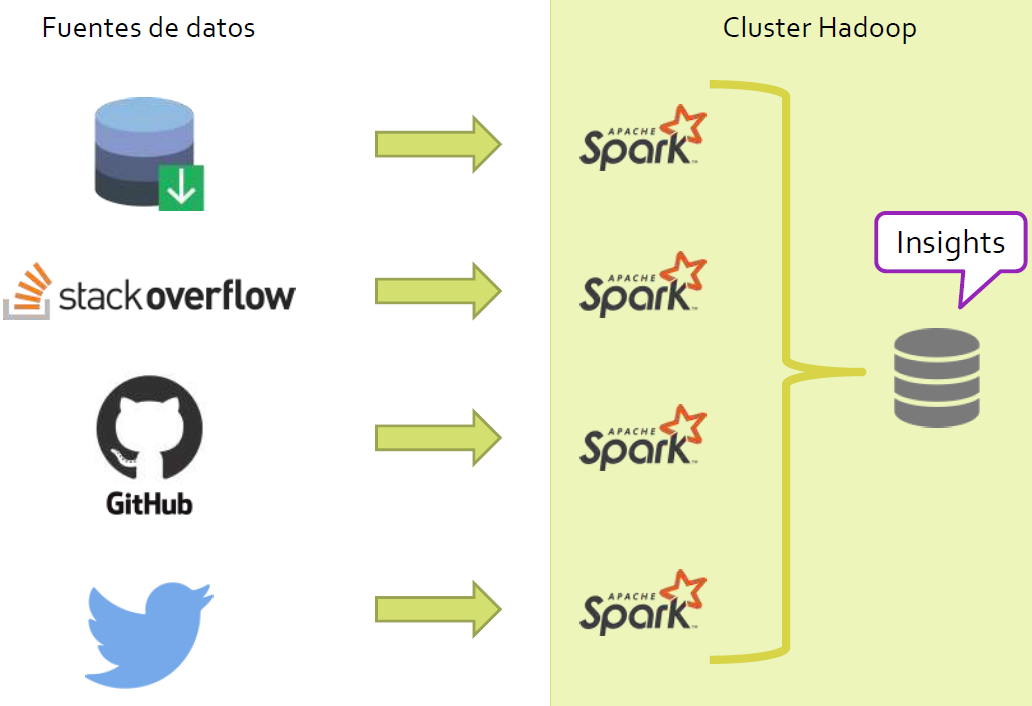
\includegraphics[scale=0.41]{graphics/dataSources}
\end{figure}

\clearpage
\section{Informe final}
\subsection{Lenguajes populares}
El primer \textit{insight} planteado corresponde a los lenguajes populares, para ello se han analizado las plataformas de Stack Overflow \cite{stackoverflow} (ver apartado \ref{sec:stackoverflow}) y GitHub \cite{github} (ver apartado \ref{sc:github}), que nos proporcionan información sobre qué preguntan los programadores y en qué trabajan respectivamente.

Como se puede observar en la figura \ref{HistGitHub} referente a la analítica de GitHub de los últimos tres años hay varios lenguajes de sobra conocidos en el sector, pero han aparecido algunos como Rust, Go, Scala o Kotlin que han adquirido una gran importancia en relativamente poco tiempo, equiparándose o superando lenguajes con varios años de bagaje, por lo que sería altamente recomendable la realización de cursos relacionados con estos lenguajes debido a su potencial y rápida aceptación por los profesionales del sector.

En la figura \ref{HistStof} se puede observar cómo algunos de los lenguajes han tenido una menor incidencia en el último año con respecto a otros anteriores, con la salvedad de Python, el cual ha aumentado su presencia en este último año pese a ser un lenguaje establecido, por lo que se prevee un relanzamiento de este en los próximos años.

En definitiva la recomendación en función de los datos sería mantener los cursos en Javascript, Java, PHP, C++, Android e Ios y aumentar o crear cursos sobre Rust, Go, Scala, Kotlin y Python.
\begin{figure}[htp!]
	\centering
	\caption{Histórico Stack Overflow}
	\label{HistStof}
	\vspace{5pt}
	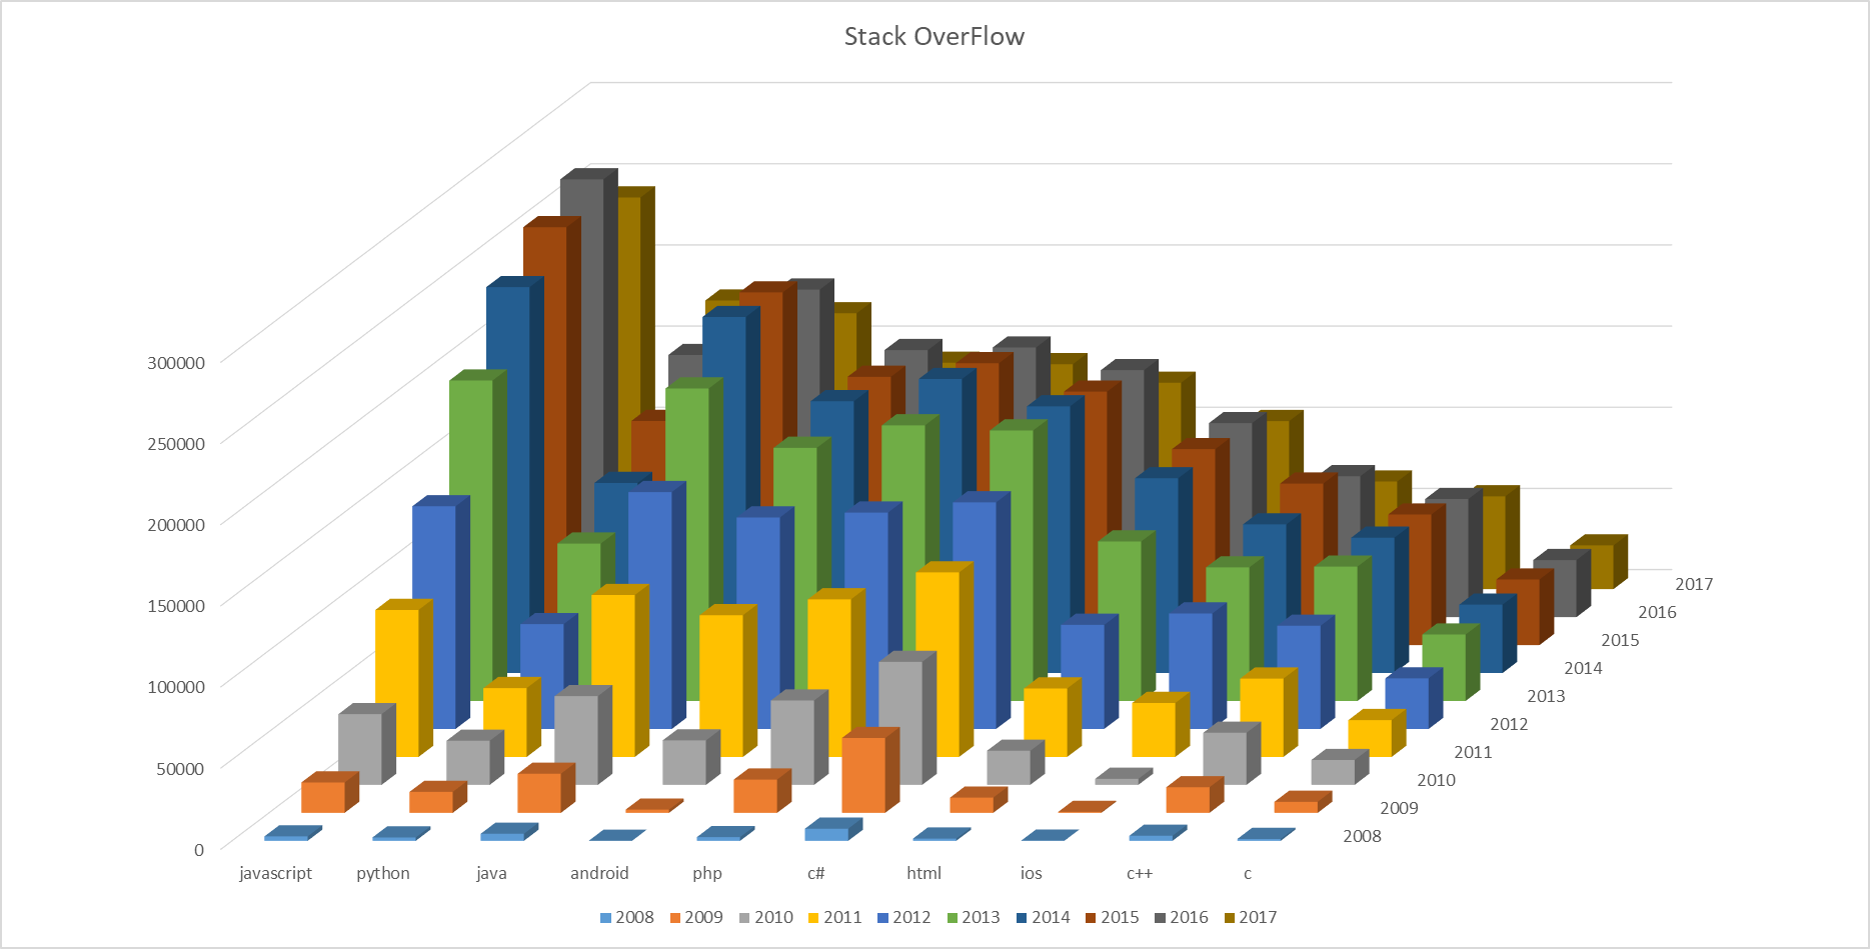
\includegraphics[scale=0.55]{graficas/stofHist}
\end{figure}
\begin{figure}[htp!]
	\centering
	\caption{Histórico de GitHub}
	\label{HistGitHub}
	\vspace{5pt}
	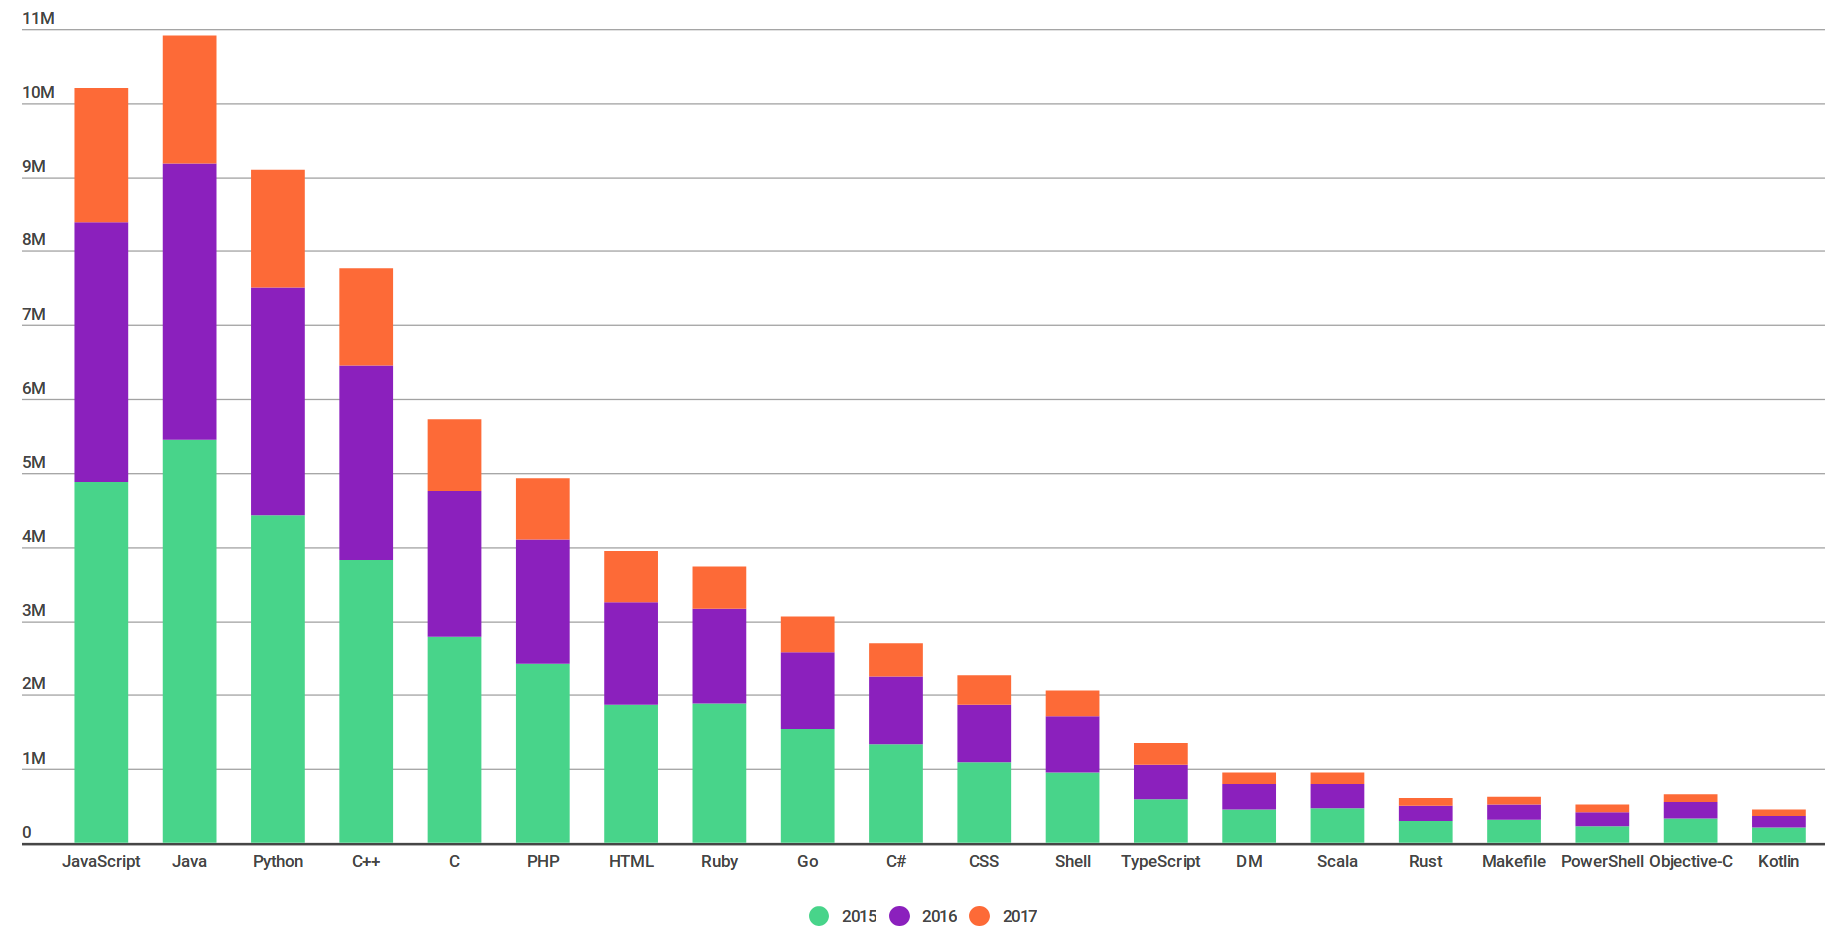
\includegraphics[scale=0.25]{graficas/githubBarTotal}
\end{figure}


\clearpage
\subsection{Regionalización de la empresa}
Otro de los \textit{insight} que solicitaba la empresa era un análisis sobre los países en los que enfocarse en caso de decidir regionalizar los cursos.
\begin{figure}[htp!]
	\centering
	\caption{Mapamundi de incidencia de programadores por país}
	\label{Mapamundi}
	\vspace{5pt}
	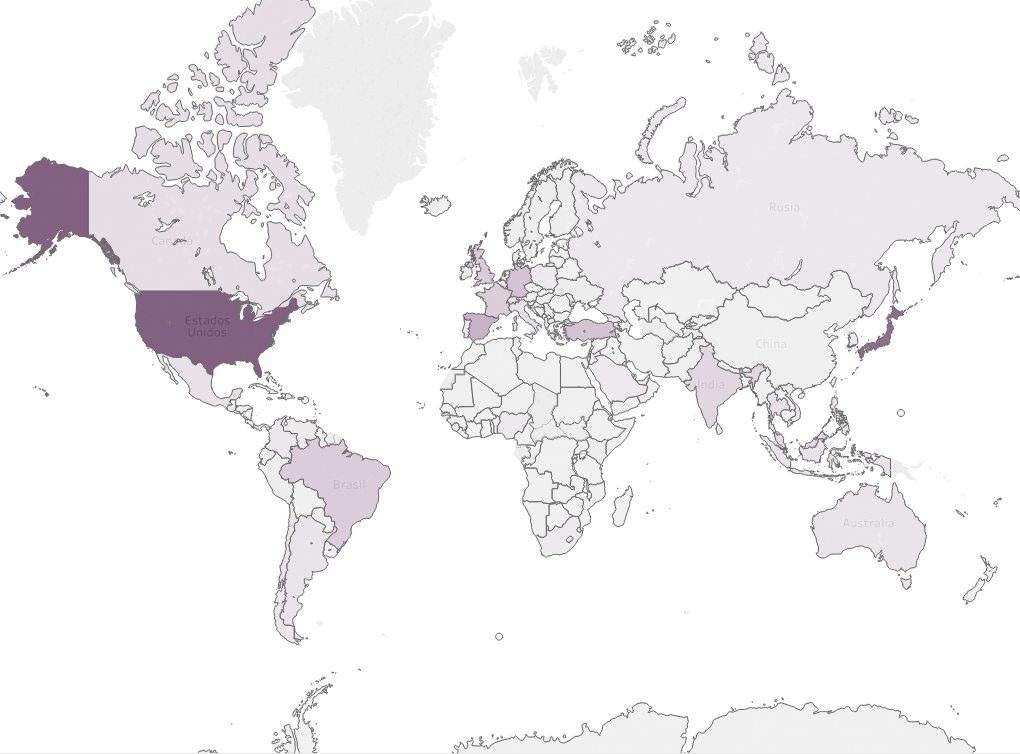
\includegraphics[scale=0.63]{graficas/CorrectMap}
\end{figure}

En la figura \ref{Mapamundi} se puede observar que la mayor incidencia se encuentra en Estados Unidos y Japón, seguido por Brasil, España, Francia, Turquía e India. La recomendación en este punto sería aumentar la presencia en estos dos países principalmente y luego expandirse hacia Europa y Sudamérica. 

Estos datos han sido extraídos de Twitter \cite{twitter}, este punto es importante ya que explica la ausencia completa de datos en China, país donde se usa la plataforma Weibo \cite{weibo} en sustitución de Twitter. Pero es un mercado de fácil acceso desde Japón sin tener que establecerse en el país.

\clearpage	
\subsection{Idioma vehicular}
\begin{figure}[htp!]
	\centering
	\caption{Gráfica orientativa sobre el uso de idiomas}
	\label{Idiomas}
	\vspace{5pt}
	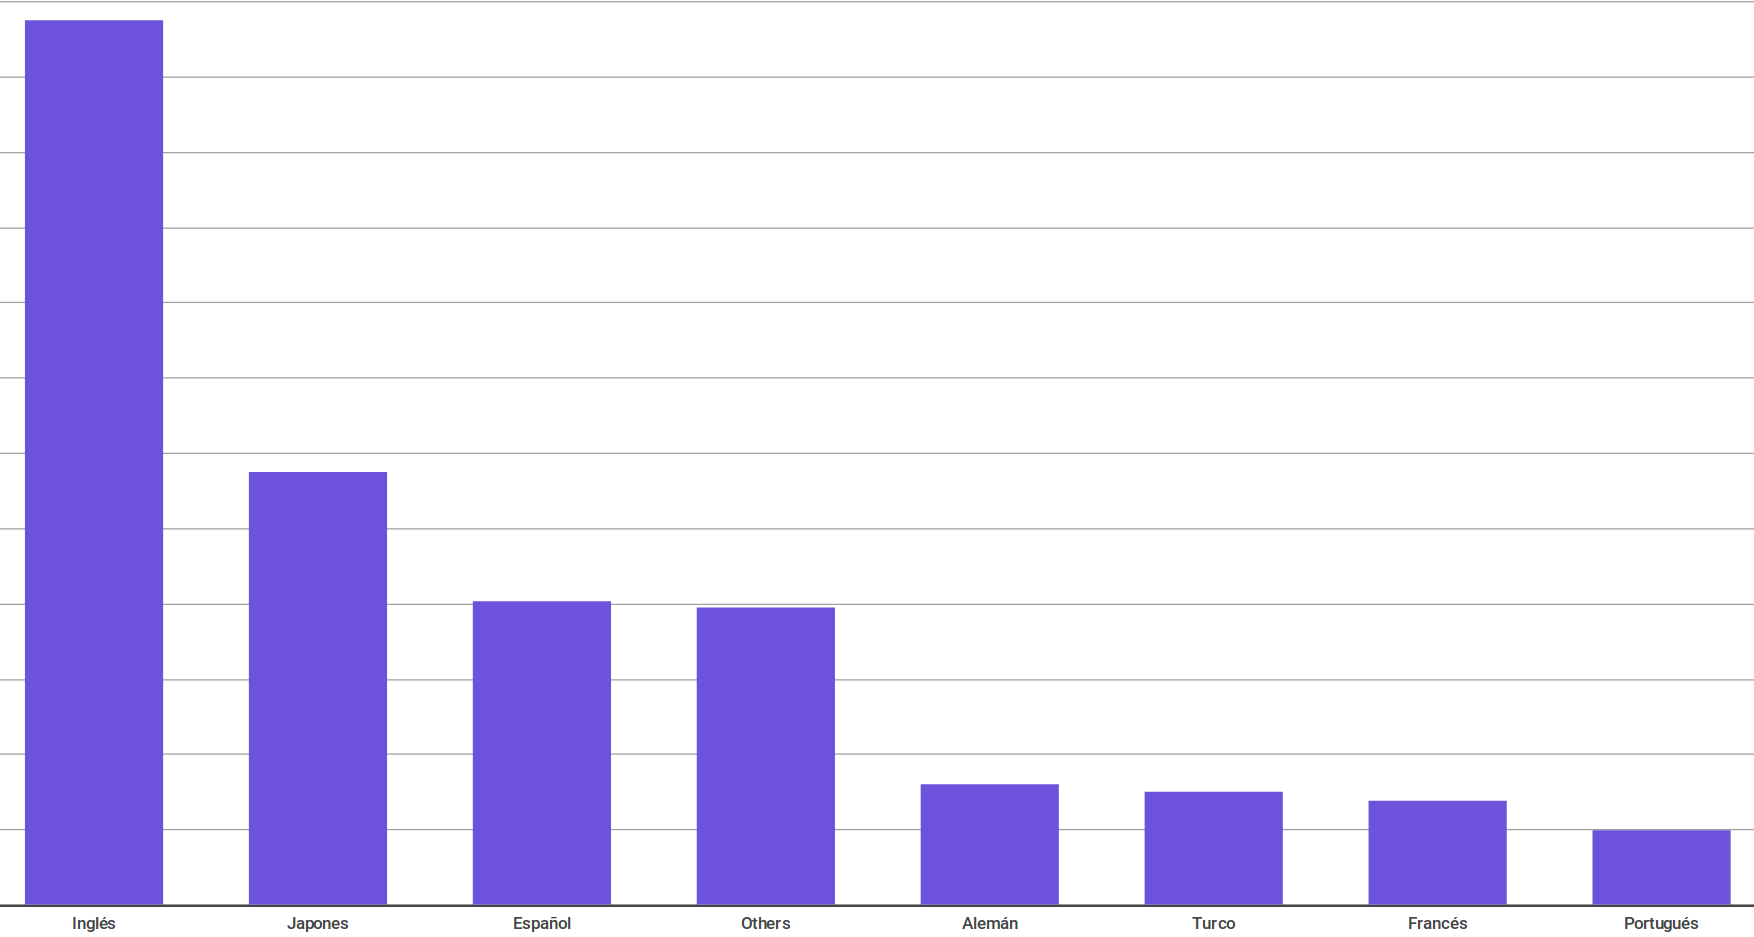
\includegraphics[scale=0.355]{graficas/LenguajesBarCorrect2}
\end{figure}

En este punto no se aprecian grandes sorpresas, el idioma principal es el inglés que además es la segunda lengua de la mayoría de los profesionales del sector, por lo que se recomienda el uso de esta para los cursos. Además, el segundo puesto lo ocupa el japones seguido del español, este primer idioma sería interesante a la hora de acercarse a una población con gran impacto tecnológico y el segundo debido al gran volumen de hispanohablantes.

El resto de idiomas tiene un impacto mucho menor, teniendo los idiomas minoritarios en conjunto un impacto similar al español.

La recomendación sería utilizar el inglés como idioma principal, asegurando la existencia de subtítulos o contenido en japonés y español para maximizar la cartera de clientes potenciales manteniendo un bajo costo por curso. 

%
% Página en blanco
%
\cleardoublepage

%
% Bibliografía
%
\printbibliography[heading=bibintoc]

% No expandir elementos para llenar toda la página
\raggedbottom

%
% Apéndices
%
\appendix
\cleardoublepage
\addappheadtotoc
\appendixpage

%
% Apéndices del TFG
%
\chapter{Estructura completa de un \textit{tweet}\label{sc:tweet}}
\lstinputlisting[basicstyle=\scriptsize, caption={Esquema completo de la estructura de un \textit{tweet}.}]{Schemas/full-tweet-struct.txt}

\cleardoublepage
\chapter{Estructura completa de un evento de GitHub\label{sc:github}}
\lstinputlisting[basicstyle=\scriptsize, caption={Esquema completo de la estructura de GitHub.}]{Schemas/full-struct-github.txt}

\cleardoublepage
\chapter{Fichero de configuración ``.bashrc'' completo\label{sc:bashrc}}
\lstinputlisting[basicstyle=\footnotesize, caption={Fichero ``.bashrc'' completo del sistema.}]{src/bashrc.txt}

% Fin del documento
\end{document}
